% Options for packages loaded elsewhere
\PassOptionsToPackage{unicode}{hyperref}
\PassOptionsToPackage{hyphens}{url}
\PassOptionsToPackage{dvipsnames,svgnames,x11names}{xcolor}
%

\documentclass[
  twocolumn]{biophys-new-mod}

\papertype{Article}


\usepackage{amsmath,amssymb}
\usepackage{lmodern}
\usepackage{iftex}
\ifPDFTeX
  \usepackage[T1]{fontenc}
  \usepackage[utf8]{inputenc}
  \usepackage{textcomp} % provide euro and other symbols
\else % if luatex or xetex
  \usepackage{unicode-math}
  \defaultfontfeatures{Scale=MatchLowercase}
  \defaultfontfeatures[\rmfamily]{Ligatures=TeX,Scale=1}
\fi
% Use upquote if available, for straight quotes in verbatim environments
\IfFileExists{upquote.sty}{\usepackage{upquote}}{}
\IfFileExists{microtype.sty}{% use microtype if available
  \usepackage[]{microtype}
  \UseMicrotypeSet[protrusion]{basicmath} % disable protrusion for tt fonts
}{}
\usepackage{xcolor}
\setlength{\emergencystretch}{3em} % prevent overfull lines
\setcounter{secnumdepth}{-\maxdimen} % remove section numbering
% Make \paragraph and \subparagraph free-standing
\ifx\paragraph\undefined\else
  \let\oldparagraph\paragraph
  \renewcommand{\paragraph}[1]{\oldparagraph{#1}\mbox{}}
\fi
\ifx\subparagraph\undefined\else
  \let\oldsubparagraph\subparagraph
  \renewcommand{\subparagraph}[1]{\oldsubparagraph{#1}\mbox{}}
\fi

\usepackage{color}
\usepackage{fancyvrb}
\newcommand{\VerbBar}{|}
\newcommand{\VERB}{\Verb[commandchars=\\\{\}]}
\DefineVerbatimEnvironment{Highlighting}{Verbatim}{commandchars=\\\{\}}
% Add ',fontsize=\small' for more characters per line
\usepackage{framed}
\definecolor{shadecolor}{RGB}{241,243,245}
\newenvironment{Shaded}{\begin{snugshade}}{\end{snugshade}}
\newcommand{\AlertTok}[1]{\textcolor[rgb]{0.68,0.00,0.00}{#1}}
\newcommand{\AnnotationTok}[1]{\textcolor[rgb]{0.37,0.37,0.37}{#1}}
\newcommand{\AttributeTok}[1]{\textcolor[rgb]{0.40,0.45,0.13}{#1}}
\newcommand{\BaseNTok}[1]{\textcolor[rgb]{0.68,0.00,0.00}{#1}}
\newcommand{\BuiltInTok}[1]{\textcolor[rgb]{0.00,0.23,0.31}{#1}}
\newcommand{\CharTok}[1]{\textcolor[rgb]{0.13,0.47,0.30}{#1}}
\newcommand{\CommentTok}[1]{\textcolor[rgb]{0.37,0.37,0.37}{#1}}
\newcommand{\CommentVarTok}[1]{\textcolor[rgb]{0.37,0.37,0.37}{\textit{#1}}}
\newcommand{\ConstantTok}[1]{\textcolor[rgb]{0.56,0.35,0.01}{#1}}
\newcommand{\ControlFlowTok}[1]{\textcolor[rgb]{0.00,0.23,0.31}{#1}}
\newcommand{\DataTypeTok}[1]{\textcolor[rgb]{0.68,0.00,0.00}{#1}}
\newcommand{\DecValTok}[1]{\textcolor[rgb]{0.68,0.00,0.00}{#1}}
\newcommand{\DocumentationTok}[1]{\textcolor[rgb]{0.37,0.37,0.37}{\textit{#1}}}
\newcommand{\ErrorTok}[1]{\textcolor[rgb]{0.68,0.00,0.00}{#1}}
\newcommand{\ExtensionTok}[1]{\textcolor[rgb]{0.00,0.23,0.31}{#1}}
\newcommand{\FloatTok}[1]{\textcolor[rgb]{0.68,0.00,0.00}{#1}}
\newcommand{\FunctionTok}[1]{\textcolor[rgb]{0.28,0.35,0.67}{#1}}
\newcommand{\ImportTok}[1]{\textcolor[rgb]{0.00,0.46,0.62}{#1}}
\newcommand{\InformationTok}[1]{\textcolor[rgb]{0.37,0.37,0.37}{#1}}
\newcommand{\KeywordTok}[1]{\textcolor[rgb]{0.00,0.23,0.31}{#1}}
\newcommand{\NormalTok}[1]{\textcolor[rgb]{0.00,0.23,0.31}{#1}}
\newcommand{\OperatorTok}[1]{\textcolor[rgb]{0.37,0.37,0.37}{#1}}
\newcommand{\OtherTok}[1]{\textcolor[rgb]{0.00,0.23,0.31}{#1}}
\newcommand{\PreprocessorTok}[1]{\textcolor[rgb]{0.68,0.00,0.00}{#1}}
\newcommand{\RegionMarkerTok}[1]{\textcolor[rgb]{0.00,0.23,0.31}{#1}}
\newcommand{\SpecialCharTok}[1]{\textcolor[rgb]{0.37,0.37,0.37}{#1}}
\newcommand{\SpecialStringTok}[1]{\textcolor[rgb]{0.13,0.47,0.30}{#1}}
\newcommand{\StringTok}[1]{\textcolor[rgb]{0.13,0.47,0.30}{#1}}
\newcommand{\VariableTok}[1]{\textcolor[rgb]{0.07,0.07,0.07}{#1}}
\newcommand{\VerbatimStringTok}[1]{\textcolor[rgb]{0.13,0.47,0.30}{#1}}
\newcommand{\WarningTok}[1]{\textcolor[rgb]{0.37,0.37,0.37}{\textit{#1}}}

\providecommand{\tightlist}{%
  \setlength{\itemsep}{0pt}\setlength{\parskip}{0pt}}\usepackage{longtable,booktabs,array}
\usepackage{calc} % for calculating minipage widths
% Correct order of tables after \paragraph or \subparagraph
\usepackage{etoolbox}
\makeatletter
\patchcmd\longtable{\par}{\if@noskipsec\mbox{}\fi\par}{}{}
\makeatother
% Allow footnotes in longtable head/foot
\IfFileExists{footnotehyper.sty}{\usepackage{footnotehyper}}{\usepackage{footnote}}
\makesavenoteenv{longtable}
\usepackage{graphicx}
\makeatletter
\def\maxwidth{\ifdim\Gin@nat@width>\linewidth\linewidth\else\Gin@nat@width\fi}
\def\maxheight{\ifdim\Gin@nat@height>\textheight\textheight\else\Gin@nat@height\fi}
\makeatother
% Scale images if necessary, so that they will not overflow the page
% margins by default, and it is still possible to overwrite the defaults
% using explicit options in \includegraphics[width, height, ...]{}
\setkeys{Gin}{width=\maxwidth,height=\maxheight,keepaspectratio}
% Set default figure placement to htbp
\makeatletter
\def\fps@figure{htbp}
\makeatother
\newlength{\cslhangindent}
\setlength{\cslhangindent}{1.5em}
\newlength{\csllabelwidth}
\setlength{\csllabelwidth}{3em}
\newlength{\cslentryspacingunit} % times entry-spacing
\setlength{\cslentryspacingunit}{\parskip}
\newenvironment{CSLReferences}[2] % #1 hanging-ident, #2 entry spacing
 {% don't indent paragraphs
  \setlength{\parindent}{0pt}
  % turn on hanging indent if param 1 is 1
  \ifodd #1
  \let\oldpar\par
  \def\par{\hangindent=\cslhangindent\oldpar}
  \fi
  % set entry spacing
  \setlength{\parskip}{#2\cslentryspacingunit}
 }%
 {}
\usepackage{calc}
\newcommand{\CSLBlock}[1]{#1\hfill\break}
\newcommand{\CSLLeftMargin}[1]{\parbox[t]{\csllabelwidth}{#1}}
\newcommand{\CSLRightInline}[1]{\parbox[t]{\linewidth - \csllabelwidth}{#1}\break}
\newcommand{\CSLIndent}[1]{\hspace{\cslhangindent}#1}

\makeatletter
\let\oldlt\longtable
\let\endoldlt\endlongtable
\def\longtable{\@ifnextchar[\longtable@i \longtable@ii}
\def\longtable@i[#1]{\begin{figure}[t]
\onecolumn
\begin{minipage}{0.5\textwidth}
\oldlt[#1]
}
\def\longtable@ii{\begin{figure}[t]
\onecolumn
\begin{minipage}{0.5\textwidth}
\oldlt
}
\def\endlongtable{\endoldlt
\end{minipage}
\twocolumn
\end{figure}}
\makeatother
\makeatletter
\@ifpackageloaded{tcolorbox}{}{\usepackage[many]{tcolorbox}}
\@ifpackageloaded{fontawesome5}{}{\usepackage{fontawesome5}}
\definecolor{quarto-callout-color}{HTML}{909090}
\definecolor{quarto-callout-note-color}{HTML}{0758E5}
\definecolor{quarto-callout-important-color}{HTML}{CC1914}
\definecolor{quarto-callout-warning-color}{HTML}{EB9113}
\definecolor{quarto-callout-tip-color}{HTML}{00A047}
\definecolor{quarto-callout-caution-color}{HTML}{FC5300}
\definecolor{quarto-callout-color-frame}{HTML}{acacac}
\definecolor{quarto-callout-note-color-frame}{HTML}{4582ec}
\definecolor{quarto-callout-important-color-frame}{HTML}{d9534f}
\definecolor{quarto-callout-warning-color-frame}{HTML}{f0ad4e}
\definecolor{quarto-callout-tip-color-frame}{HTML}{02b875}
\definecolor{quarto-callout-caution-color-frame}{HTML}{fd7e14}
\makeatother
\makeatletter
\makeatother
\makeatletter
\makeatother
\makeatletter
\@ifpackageloaded{caption}{}{\usepackage{caption}}
\AtBeginDocument{%
\ifdefined\contentsname
  \renewcommand*\contentsname{Table of contents}
\else
  \newcommand\contentsname{Table of contents}
\fi
\ifdefined\listfigurename
  \renewcommand*\listfigurename{List of Figures}
\else
  \newcommand\listfigurename{List of Figures}
\fi
\ifdefined\listtablename
  \renewcommand*\listtablename{List of Tables}
\else
  \newcommand\listtablename{List of Tables}
\fi
\ifdefined\figurename
  \renewcommand*\figurename{Figure}
\else
  \newcommand\figurename{Figure}
\fi
\ifdefined\tablename
  \renewcommand*\tablename{Table}
\else
  \newcommand\tablename{Table}
\fi
}
\@ifpackageloaded{float}{}{\usepackage{float}}
\floatstyle{ruled}
\@ifundefined{c@chapter}{\newfloat{codelisting}{h}{lop}}{\newfloat{codelisting}{h}{lop}[chapter]}
\floatname{codelisting}{Listing}
\newcommand*\listoflistings{\listof{codelisting}{List of Listings}}
\makeatother
\makeatletter
\@ifpackageloaded{caption}{}{\usepackage{caption}}
\@ifpackageloaded{subcaption}{}{\usepackage{subcaption}}
\makeatother
\makeatletter
\@ifpackageloaded{tcolorbox}{}{\usepackage[many]{tcolorbox}}
\makeatother
\makeatletter
\@ifundefined{shadecolor}{\definecolor{shadecolor}{rgb}{.97, .97, .97}}
\makeatother
\makeatletter
\makeatother
\ifLuaTeX
  \usepackage{selnolig}  % disable illegal ligatures
\fi
\IfFileExists{bookmark.sty}{\usepackage{bookmark}}{\usepackage{hyperref}}
\IfFileExists{xurl.sty}{\usepackage{xurl}}{} % add URL line breaks if available
\urlstyle{same} % disable monospaced font for URLs
\hypersetup{
  pdftitle={Intrinsically disordered region of Talin's FERM domain functions as an initial PIP2 recognition site},
  pdfauthor={Jannik Buhr; Florian Franz; Frauke Gräter},
  pdfkeywords={Molecular Dynamics, Talin, Focal
Adhesion, Mechanosensing, Disorder, IDP, IDR},
  colorlinks=true,
  linkcolor={blue},
  filecolor={Maroon},
  citecolor={Blue},
  urlcolor={Blue},
  pdfcreator={LaTeX via pandoc}}


\title{Intrinsically disordered region of Talin's FERM domain functions
as an initial PIP\textsubscript{2} recognition site}
\runningtitle{Intrinsically disordered region of Talin's FERM domain
functions as an initial PIP\textsubscript{2} recognition site}

  \author[1,2,*]
  {Jannik Buhr}
  \author[1,2]
  {Florian Franz}
  \author[1,2]
  {Frauke Gräter}

\affil[1]{Heidelberg Institute for Theoretical Studies}
\affil[2]{Interdisciplinary Center for Scientific Computing, Heidelberg
University}

  \corrauthor[*]{jannik.buhr@h-its.org}

\runningauthor{Jannik Buhr, Florian Franz, Frauke Gräter}

\begin{document}
\begin{frontmatter}

\begin{abstract}
Focal adhesions (FAs) mediate the interaction of the cytoskeleton with
the extracellular matrix (ECM) in a highly dynamic fashion. Talin is a
central regulator, adaptor protein and mechano-sensor of focal adhesion
complexes. For recruitment and firm attachment at FAs, Talin's
N-terminal FERM domain binds to phosphatidylinositol 4,5-bisphosphate
(PIP\textsubscript{2})-enriched membranes. A newly published
autoinhibitory structure of Talin, where the known PIP\textsubscript{2}
interaction sites are covered up, lead us to hypothesize that a hitherto
less examined loop insertion of the FERM domain acts as an additional
and initial site of contact. We evaluated direct interactions of Talin
with the membrane lipid PIP\textsubscript{2} by means of atomistic
molecular dynamics (MD) simulations. We show that this unstructured,
33-residue-long loop strongly interacts with PIP\textsubscript{2} and
can facilitate further interactions by serving as a flexible membrane
anchor. Under physiological force as present in Talin at FAs, the
extensible FERM loop ensures Talin to maintain membrane contacts when
pulled away from the membrane by up to 7nm. This work presents the
dynamics of the interaction and identifies key residues. Our results put
forward an intrinsically disordered loop as a key and highly adaptable
PIP\textsubscript{2} recognition site of Talin and potentially other
PIP\textsubscript{2}-binding mechano-proteins.
\end{abstract}


\begin{sigstatement}
TODO Each manuscript must also have a statement of significance or no
more than 120 words.
\end{sigstatement}


\end{frontmatter}\ifdefined\Shaded\renewenvironment{Shaded}{\begin{tcolorbox}[breakable, borderline west={3pt}{0pt}{shadecolor}, sharp corners, enhanced, boxrule=0pt, interior hidden, frame hidden]}{\end{tcolorbox}}\fi

\begin{tcolorbox}[enhanced jigsaw, arc=.35mm, colbacktitle=quarto-callout-warning-color!10!white, colback=white, left=2mm, breakable, colframe=quarto-callout-warning-color-frame, bottomrule=.15mm, leftrule=.75mm, rightrule=.15mm, title=\textcolor{quarto-callout-warning-color}{\faExclamationTriangle}\hspace{0.5em}{Warning}, bottomtitle=1mm, opacitybacktitle=0.6, toprule=.15mm, opacityback=0, coltitle=black, toptitle=1mm, titlerule=0mm]
This is a draft and as such subject to change.
\end{tcolorbox}

\begin{tcolorbox}[enhanced jigsaw, arc=.35mm, colbacktitle=quarto-callout-tip-color!10!white, colback=white, left=2mm, breakable, colframe=quarto-callout-tip-color-frame, bottomrule=.15mm, leftrule=.75mm, rightrule=.15mm, title=\textcolor{quarto-callout-tip-color}{\faLightbulb}\hspace{0.5em}{Tip}, bottomtitle=1mm, opacitybacktitle=0.6, toprule=.15mm, opacityback=0, coltitle=black, toptitle=1mm, titlerule=0mm]

The source repository for this paper lives
\href{https://github.com/hits-mbm-dev/paper-talin-loop}{here}. The pdf
version of this paper lives \href{./index.pdf}{here}.

You can find the poster that goes along with the paper presented at the
\href{https://www.biophysics.org/2022meeting\#}{Annual Meeting of the
Biophysical Society 2022} in your favorite format here:

\begin{itemize}
\tightlist
\item
  \href{./poster.html}{poster web/html}
\item
  \href{./poster.pdf}{poster print/pdf}
\end{itemize}

\end{tcolorbox}

\hypertarget{introduction}{%
\section{Introduction}\label{introduction}}

Cells critically sense the mechanics of their enviroment at cell
adhesion sites for a multitude of biological processes. Contact with the
extracellular matrix and surrounding cells regulates growth,
differentiation, motility and even apoptosis (1--4). The multiprotein
focal adhesion complex is responsible for translating and integrating
between biochemical and mechanical signals for both outside--in and
inside--out activation(5, 6).

At the center of the focal adhesion complex sits the adaptor protein
Talin, which dynamically unfolds and refolds under force (7). A
schematic of Talin can be seen in Figure~\ref{fig-tln-schema-long}.
Through interaction with integrin tails (dark green) (8), which in turn
interact with collagen fibers via their heads, it links the
extracellular matrix to the intracellular cytoskeleton by directly
interacting with actin. Talin also features specific interactions with
the membrane. Their formation, mechanical stability and role in
mechanosensing remain to be fully resolved.

Talin features an N-terminal FERM domain (F for 4.1 protein, E for
ezrin, R for radixin and M for moesin), which is composed of the
subdomains F0 to F3 and provides a link to the cystosolic side of the
plasma membrane (9). It does so via a conserved binding motif for
phosphatidylinositol 4,5-bisphosphate (PIP\textsubscript{2}), which is
enriched at active focal adhesion sites (10--12). The main
PIP\textsubscript{2} binding sites are located in F2 and F3 (highlighted
as red spheres in Figure~\ref{fig-tln-schema-long}).

Notably, the Talin1 FERM domain differs from other FERM proteins through
the addition of the F0 subdomain, which is connected to F1 via a charged
interface, as well as an insertion in F1, a flexible loop with helical
propensity and basic residues (13). Additionally, Talin's FERM domain
exists in an extended conformation, as opposed to the cloverleaf-like
conformation of other FERM proteins (14). F3 also has a binding site for
\(\beta\)-integrin tails (15) and is partly responsible for the
enrichment of PIP\textsubscript{2} at the membrane through a binding
site for PIPKI\(\gamma\) (16). A second integrin binding site is located
in the rod domain 11 (R11) (17). Talin interacts with the cytoskeleton
through actin binding sites (F2-F3, R4-R8, R13-DH) (18). The review by
Klapholz et al. (19) provides an excellent overview of the many
interaction sites of Talin and their central role in the focal adhesion
complex.

The mechanistic role of the disordered F1 loop in the many aspects of
Talin function remains elusive. Its overall positive charge renders it a
prime candidate as a PIP\textsubscript{2} binding site. However,
previous studies only identified a minor role of the loop in
PIP\textsubscript{2} binding compared to F2-F3 (20, 21). On the other
hand, the F1 loop has been shown to contribute to Talin-mediated
integrin activation (13).

It was previously shown that F3 can interact with R9, which impedes
integrin activation (22). Furthermore, in a recently determined
cryo-electron microscopy structure of autoinhibited Talin1, Dedden et
al. (23) showed that the rod domains R9 and R12 shield the established
PIP\textsubscript{2} binding surface and the integrin binding site in F3
(see
Figure~\ref{fig-tln-schema-autoinhib}, Figure~\ref{fig-tln-align-autoinhib}).
This beckons the question how this autoinhibition can be resolved. Song
at al. (12) previously investigated a fragment of Talin consisting of
F2-F3 and an inhibiting rod segment and suggested a pull-push mechanism,
whereby negatively charged PIP\textsubscript{2} attracts its positively
charged binding surface on F2-F3 and simultaneously repels the
negatively charged surface of the inhibitive rod segment. However, this
still leaves open the question of how Talin can establish a first
contact with the membrane and remain within a sufficient proximity for
this effect to kick in.

\begin{figure}

\begin{minipage}[t]{\linewidth}

{\centering 

\raisebox{-\height}{

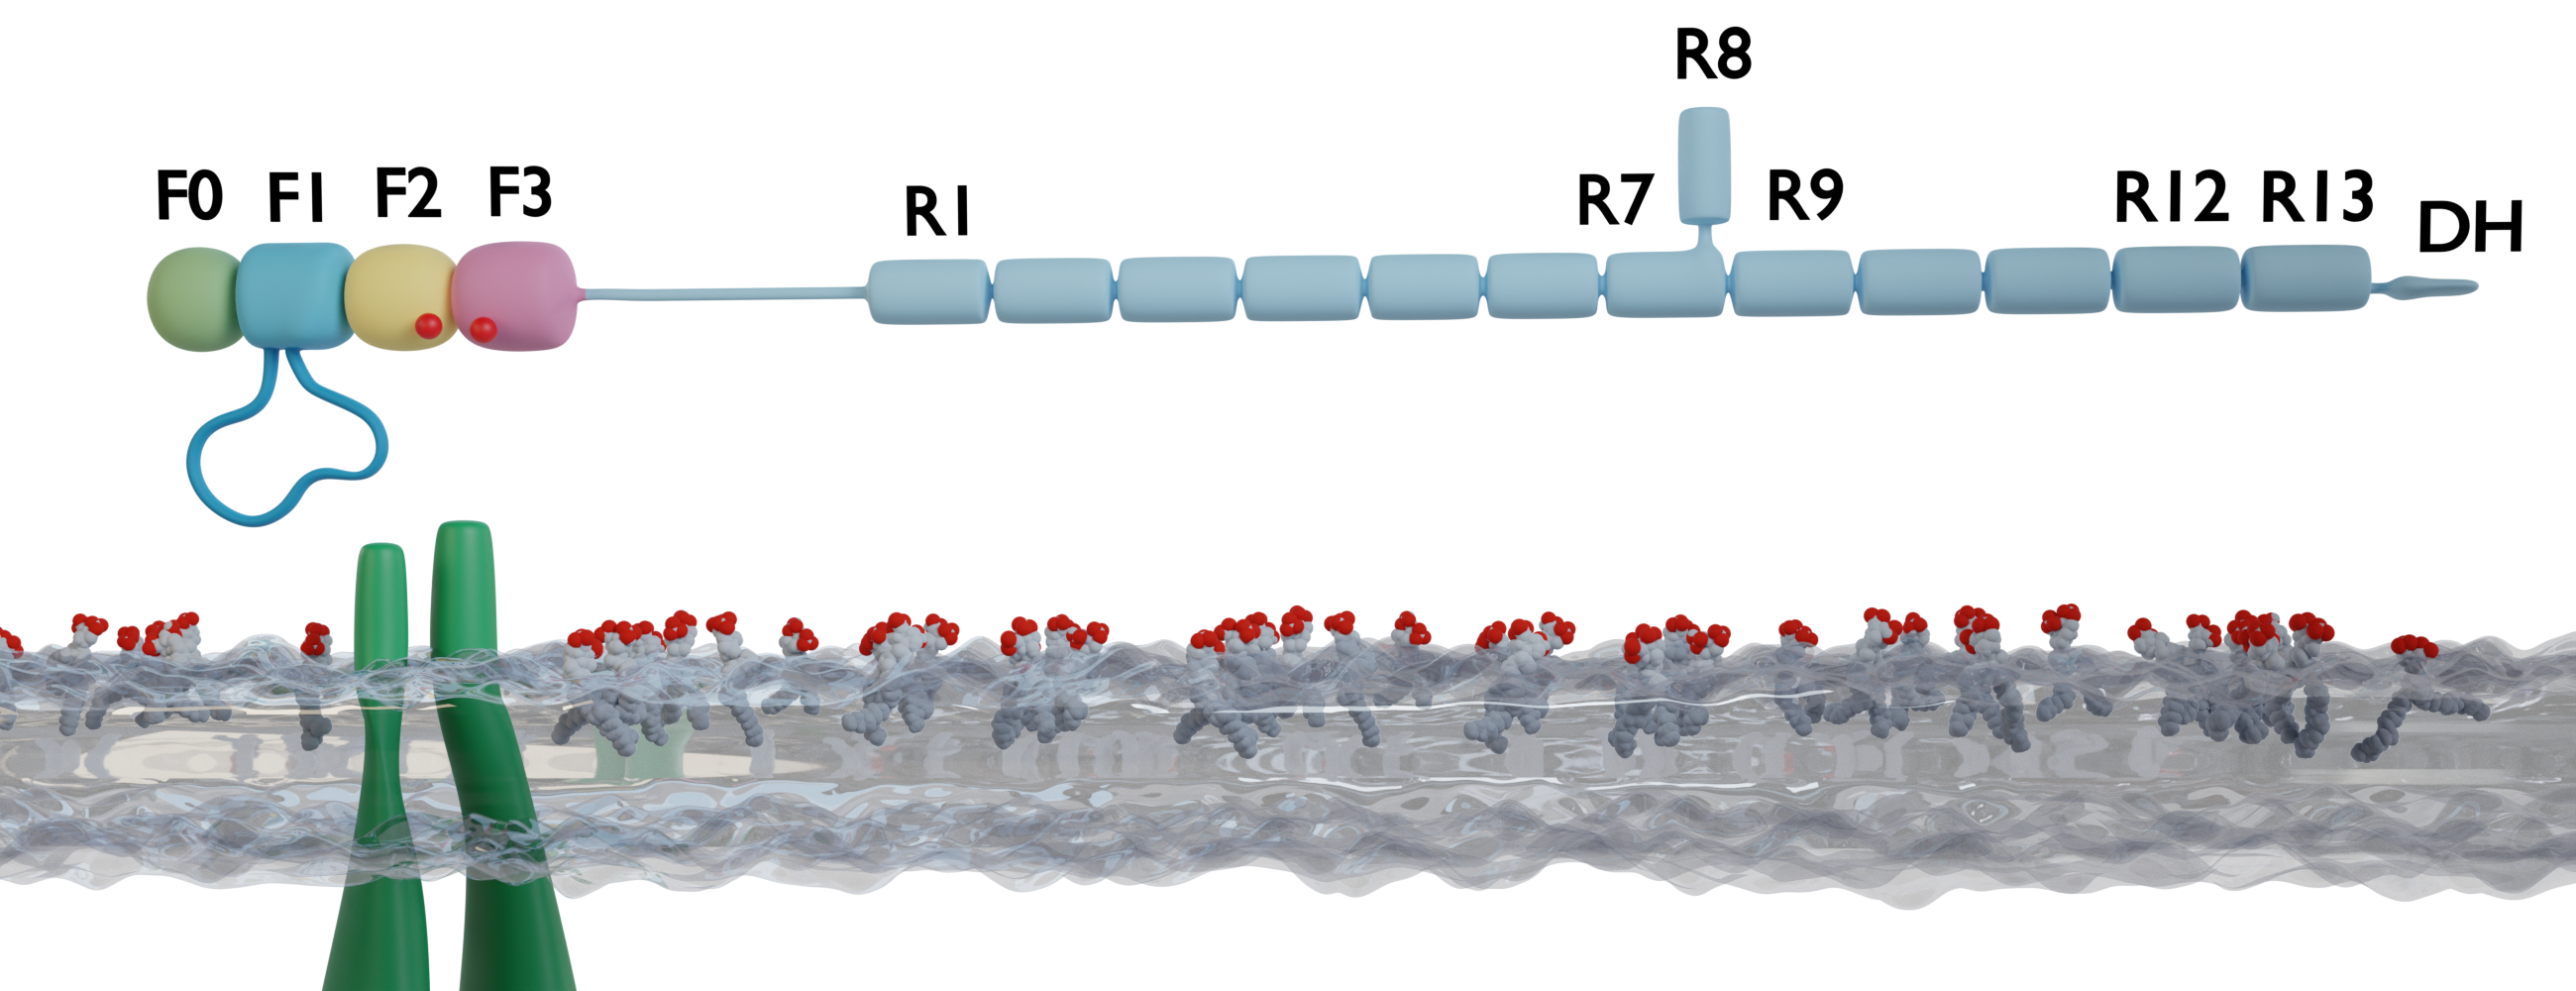
\includegraphics{./assets/blender/render/frame0000.png}

}

}

\subcaption{\label{fig-tln-schema-long}~}
\end{minipage}%
\newline
\begin{minipage}[t]{0.50\linewidth}

{\centering 

\raisebox{-\height}{

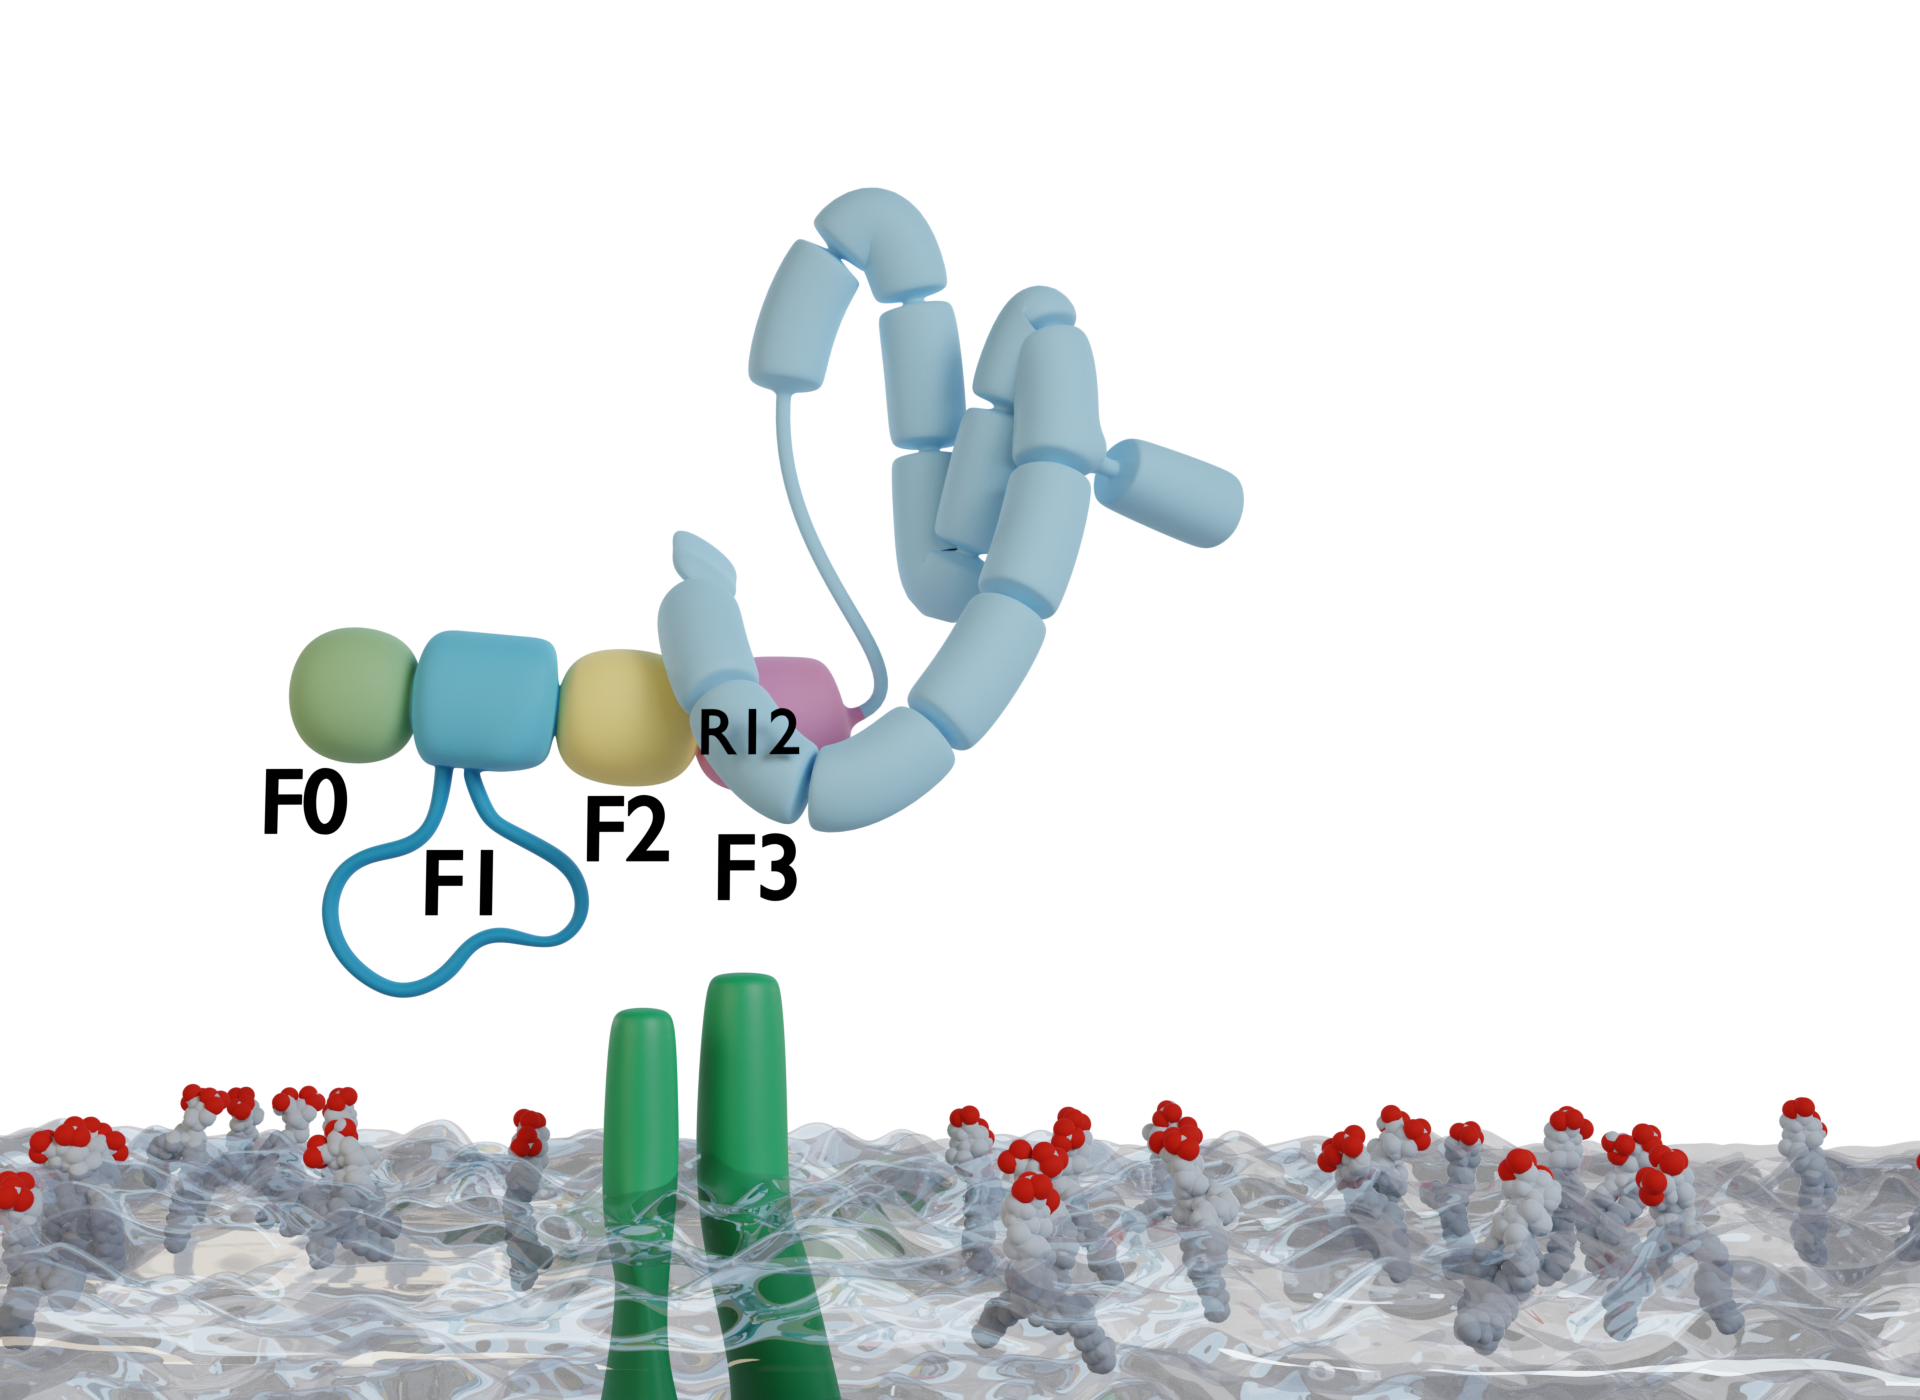
\includegraphics{./assets/blender/render/frame0001.png}

}

}

\subcaption{\label{fig-tln-schema-autoinhib}~}
\end{minipage}%
%
\begin{minipage}[t]{0.50\linewidth}

{\centering 

\raisebox{-\height}{

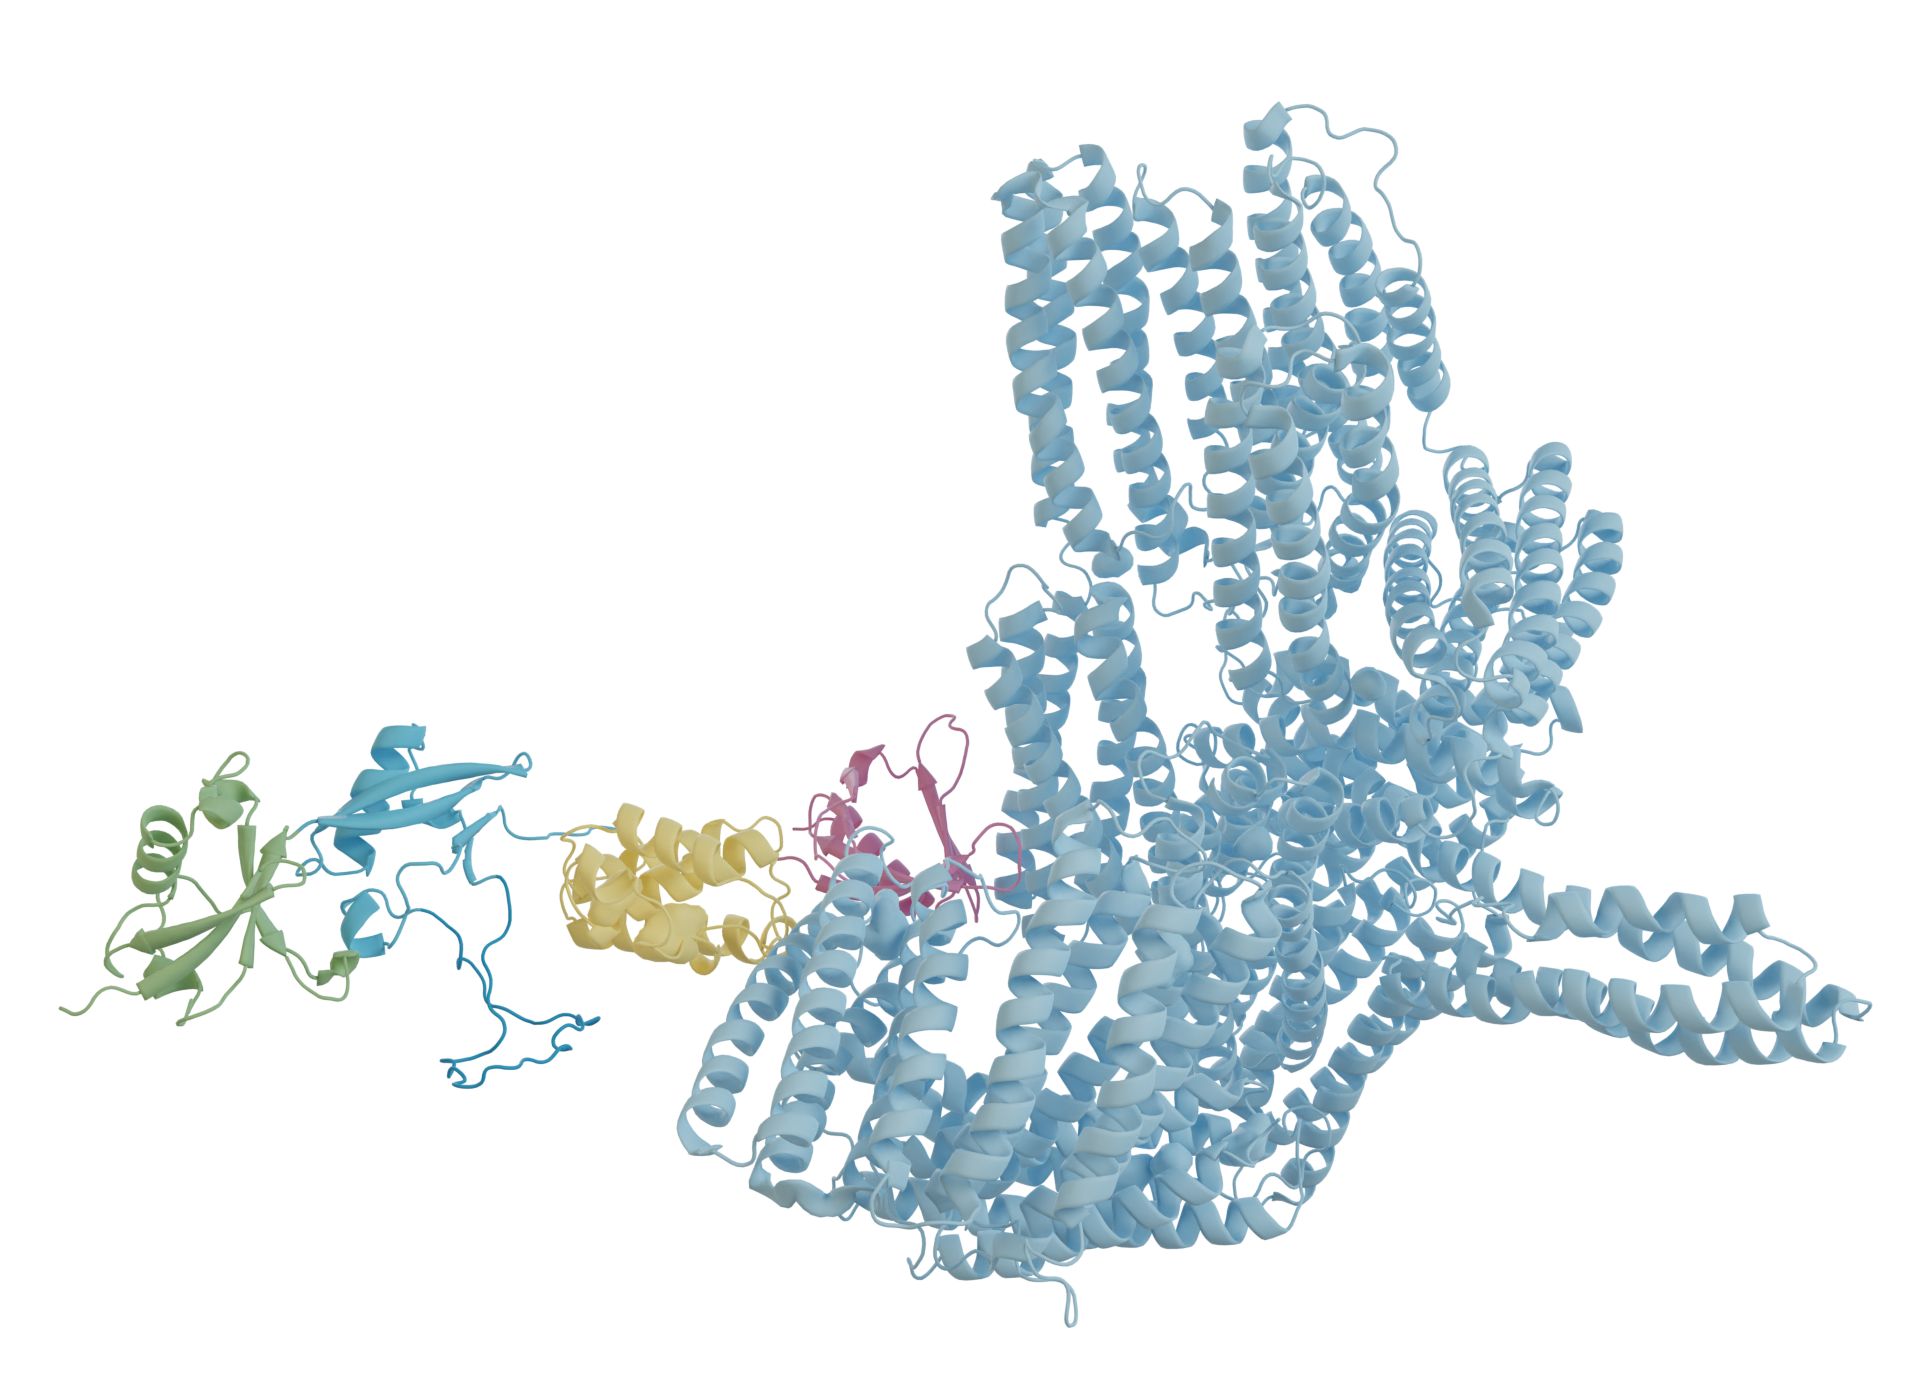
\includegraphics{./assets/blender/render-align/frame0000.png}

}

}

\subcaption{\label{fig-tln-align-autoinhib}~}
\end{minipage}%

\caption{\label{fig-structure}A schematic overview of Talin and our
simulation setup. \textbf{a)} A schematic rendering of full-length Talin
over a POPC membrane enriched with PIP\textsubscript{2} in the upper
leaflet. The subdomains under scrutiny in this publication, namely
F0-F3, which comprise the N-terminal FERM domain (or Talin head), are
highlighted in pastel colors (green, cyan, yellow, magenta). The two
major PIP\textsubscript{2} binding sites in F2-F3 are marked with red
spheres. The Talin rod segments (or Talin tail) are numbered R1 to R13.
Note that under physiological conditions, with Talin experiencing force
from bound actin, the angle between the FERM domain and the Talin rod
would be more akin to 30° as opposed to the linear structure shown here
for illustrative purposes. Tails of an integrin \(\alpha\) and \(\beta\)
heterodimer reaching through the lipid bilayer are represented in green.
\textbf{b)} A schematic rendering of the autoinhibited structure of
Talin as crystallized by Dedden et al. (23) in combination with a
cartoon representation in \textbf{c)}. The completed FERM structure by
Elliott et al. (14), with our addition of the modelled F1 loop, is
fitted to the autoinhibited structure, as the latter does not include
F0-F1 due to their flexibility. The complete FERM structure can be
explored interactively in the context of our simulation system in the
Supplementary Materials. The main PIP\textsubscript{2}-binding sites in
F2-F3 are occluded by rod domain 12.}

\end{figure}

We hypothesized that the flexible F1 loop inserted into Talin's FERM
domain serves as an additional PIP\textsubscript{2} interaction site. As
such it would be readily accessible to PIP\textsubscript{2} even in
Talin's autoinhibited conformation and would further mechanically
stabilize Talin's interaction with the membrane. To test this
hypothesis, we modelled the loop, which, due to its high flexibility, is
not included in crystal structures of the FERM domain, such as PDB-ID
3IVF by Elliot et al. (14).

With a complete structure of the Talin FERM domain we investigated the
role of the F1 loop through atomistic molecular dynamics (MD)
simulations, which had previously also proven useful to detect the
recognition of PIP\textsubscript{2} in membranes by PH domains (24) or
the FERM domain of Focal Adhesion Kinase (25).

In F0-F1 simulations, we found the loop to have a clear propensity to
interact with the PIP\textsubscript{2}-containing membrane. It is able
to establish a first contact with the membrane even from unfavorable
initial orientations due to its large search volume. Furthermore, we
show with simulations of the full-length FERM domain that once the loop
has established an initial contact, it can anchor the FERM domain to the
membrane and establish the known major binding sites in F2-F3.

These results provide mechanistic insight Talin--PIP\textsubscript{2}
interactions and highlight the role of secondary intrinsically
disordered binding surfaces for membrane recognition.

\hypertarget{materials-and-methods}{%
\section{Materials and Methods}\label{materials-and-methods}}

\hypertarget{molecular-dynamics-with-gromacs}{%
\subsection{Molecular dynamics with
GROMACS}\label{molecular-dynamics-with-gromacs}}

MD simulations were performed with GROMACS (26, 27) version 2020.03
(28). A crystal structure of the Talin FERM domain by Elliot et al. (14)
with the PDB-ID 3IVF was used as the basis of all simulations.

The missing F1 domain loop between residues L133 and W144 was modeled
using MODELLER (29, 30) via the interface to Chimera (31), followed by
equilibration with GROMACS. The resulting conformation was compared to
an NMR structure of the F1 domain (PDB-ID 2KC2) by Goult et al. (13).

The missing residue M1 was also added. The missing residues I399 and
L400 were not modeled, leaving us with a continuous sequence from
residue 1 to 398. Simulations were performed with the CHARM36 force
field. Topologies, including the membrane, were generated with the
CHARM-GUI web app (32--34) and GROMACS tools. All simulations used the
TIP3P water model and were neutralized with 0.15 mol/L of NaCl. A 6-step
equilibration was performed after gradient decent energy minimization
while gradually relieving restraints on protein and membrane atoms.
Production runs used a timestep of 2 fs, a Verlet cut-off scheme for
Van-der-Waals interactions and the Particle Mesh Ewald (PME) method for
long-range electrostatics. NPT-ensembles were achieved by Nosé-Hoover
temperature coupling (35, 36) and Parinello-Rahman pressure coupling
(37). An example \texttt{.mdp}-file can be found in the Supplementary
Materials.

The initial equilibrium simulation of the completed FERM domain was run
for 75 ns. Subsequently, the root mean squared fluctuation (RMSF) was
calculated with GROMACS tools.

The F0F1 FERM sub domains (residues 1 to 197) were simulated to evaluate
protein-membrane association using a rotational sampling approach. This
entailed placing the protein 1.5 nm away from a
1-palmitoyl-2-oleoyl-glycero-3-phosphocholine (POPC) membrane in a total
of 60 orientations spanning a rotation of 360 degrees. 6 replicates of
each orientation were run for 200~ns each. However, due to a hardware
failure, 6 of these 360 runs are only 50 to 150~ns long. Of the 119
lipids in the upper leaflet of the POPC membrane, 12 lipids were
replaced with PIP\textsubscript{2}, which results in a physiological
concentration of 10\% PIP\textsubscript{2}.

From this rotational sampling, we selected representative conformations
with loop-membrane interactions as the basis of 6 equilibrium
simulations of the complete FERM domain over a POPC membrane with 26
PIP\textsubscript{2} lipids out of a total of 273 lipids in the upper
leaflet. Each simulation ran for 400~ns. The initial conformations for
perpendicular pulling simulations of the F0F1 subdomains to gauge
interaction strength were also chose from the rotational sampling set.

Distance information was extracted from trajectories with gromacs tools
interfaced via CONAN (38).

\hypertarget{automation-data-analysis-and-availability}{%
\subsection{Automation, Data Analysis and
Availability}\label{automation-data-analysis-and-availability}}

Setup scripts written in bash are available for all simulations shown in
this work. Computations for data analysis were tracked with the targets
R package (39). Plots were generated with ggplot2 (40). Interactive
structure representations are embedded using Mol* (41). Schematic
visualizations were rendered with blender (42) and VMD (43). Files
relevant to this paper that are too big to be uploaded to this
repository, such as trajectories and blender files, will be uploaded to
a separate location. This paper and the matching poster were generated
with \href{https://quarto.org/}{quarto} (44--46).

\hypertarget{results}{%
\section{Results}\label{results}}

\hypertarget{the-f1-loop-can-act-as-a-point-of-first-contact}{%
\subsection{The F1 loop can act as a point of first
contact}\label{the-f1-loop-can-act-as-a-point-of-first-contact}}

The high flexibility of the F1 loop gave use the confidence to model it
from sequence It retained its flexibility in equilibrium simulations
(Figure~\ref{fig-loop-rmsf}), which in combination with comparisons to
NMR structures (13) confirmed this approach. The resulting system that
provides the basis for our simulations can be explored interactively in
the Supplementary Materials.

When simulating only F0-F1 over a POPC membrane containing 10\%
PIP\textsubscript{2}, we noticed that the F1 loop had a clear propensity
to establish contact with the membrane. And once contact had been
established the protein was anchored strongly enough for more contacts
to evolve with time, pulling the protein onto the membrane (see
Figure~\ref{fig-f0f1-unbound}, \ref{fig-f0f1-anchored}, \ref{fig-f0f1-bound}).
In order to control for a potential bias towards the loop as a result of
the starting position we performed a rotational sampling of the system,
where the starting angle of the loop with respect to the membrane was
varied across 60 equally spaced angles. Figure~\ref{fig-f0f1-ri-angle}
shows that independent of the starting position, the loop is able to
find the membrane and bind to it, though this does happen earlier in the
simulation when the loop starts favorably oriented towards the membrane
(Figure~\ref{fig-f0f1-angle-frame}). However, even in its most
unfavorable starting orientation (180°, oriented away from the membrane)
the loop is able to find the membrane due to the large search space it
can cover with its high flexibility (see Figure~\ref{fig-loop-rmsf}).

Once contact has been made, it becomes exceedingly unlikely for F0-F1 to
dissociate from the membrane (Figure~\ref{fig-f0f1-retention}). Of 358
runs \footnote{6 replicas each for 60 angles minus 2 runs lost to a
  storage failure}, 89 runs never made contact with the membrane, but
out of the 269 that did, only 10 eventually dissociated.

Figure~\ref{fig-f0f1-ri-npip} highlights the residues involved in the
interaction.

\begin{figure}

\begin{minipage}[t]{0.33\linewidth}

{\centering 

\raisebox{-\height}{

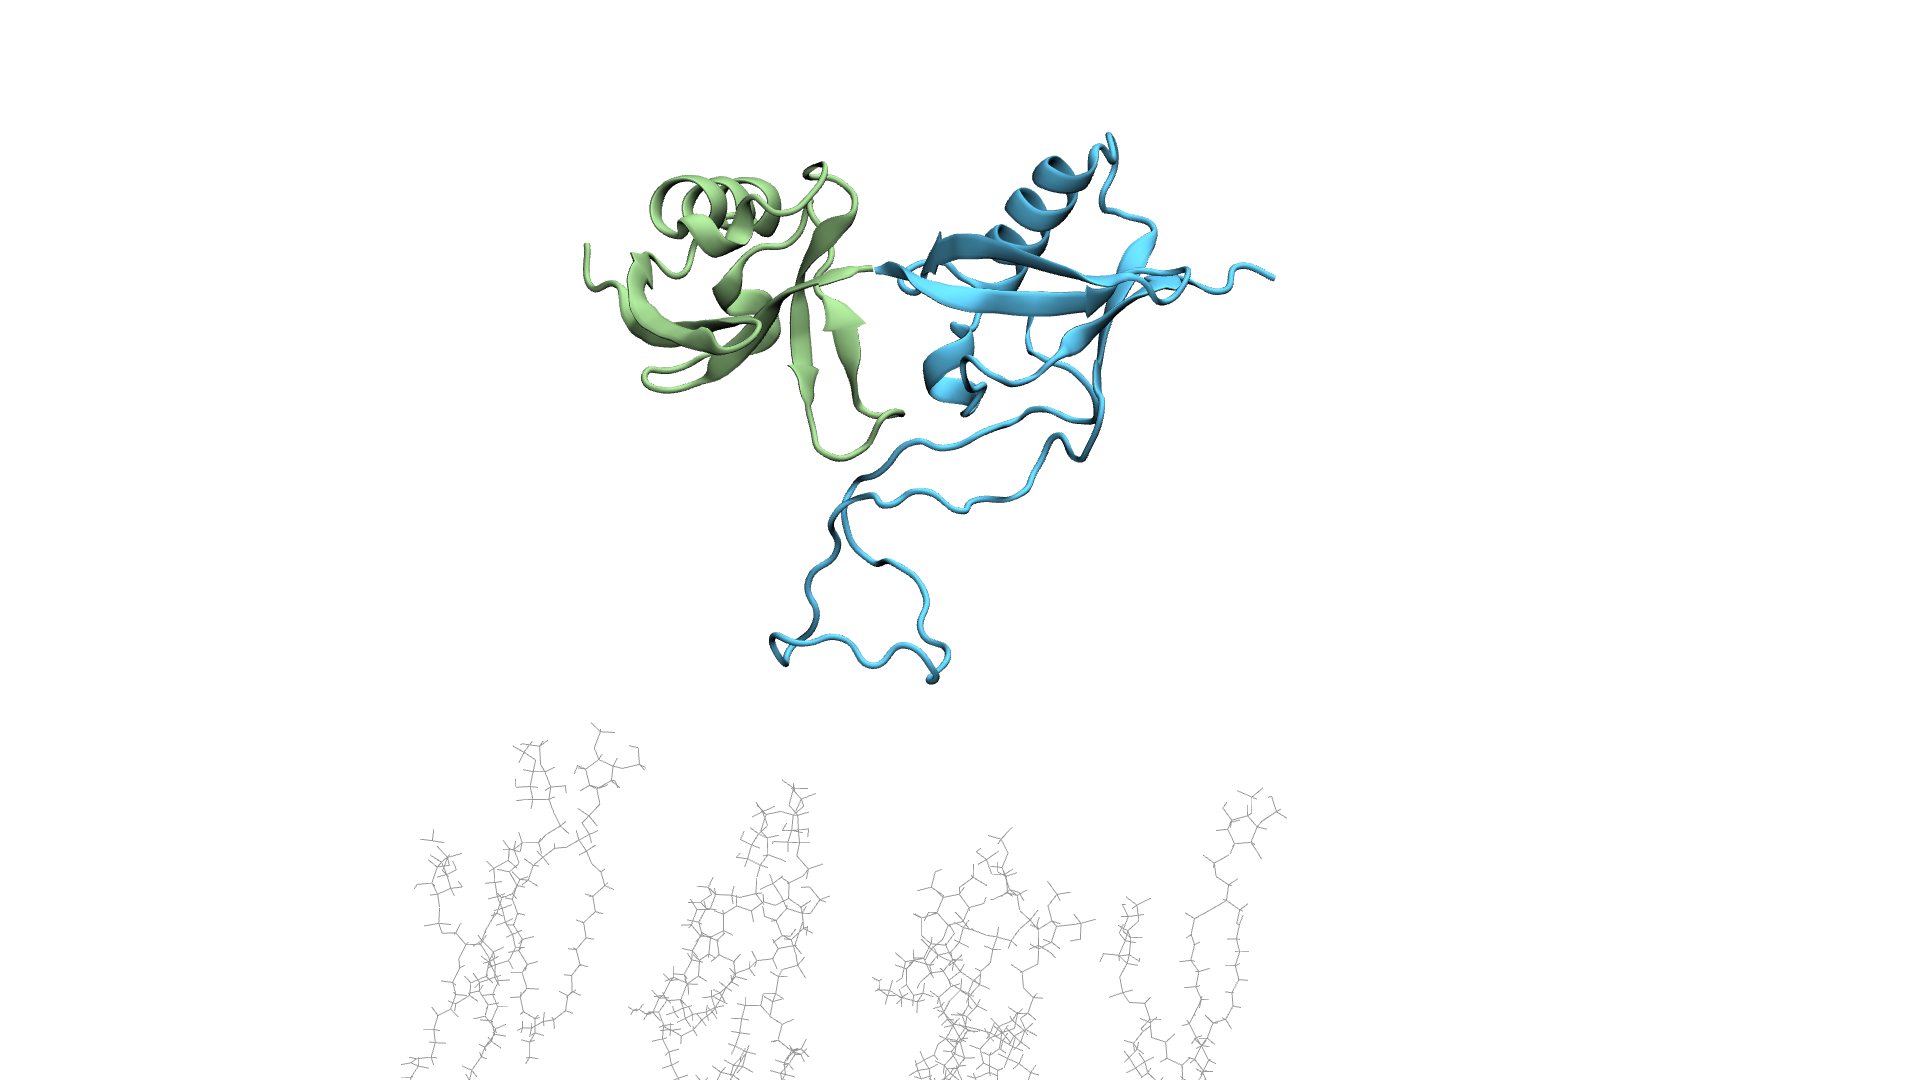
\includegraphics{./assets/vmd/f0f1/unbound.png}

}

}

\subcaption{\label{fig-f0f1-unbound}~}
\end{minipage}%
%
\begin{minipage}[t]{0.33\linewidth}

{\centering 

\raisebox{-\height}{

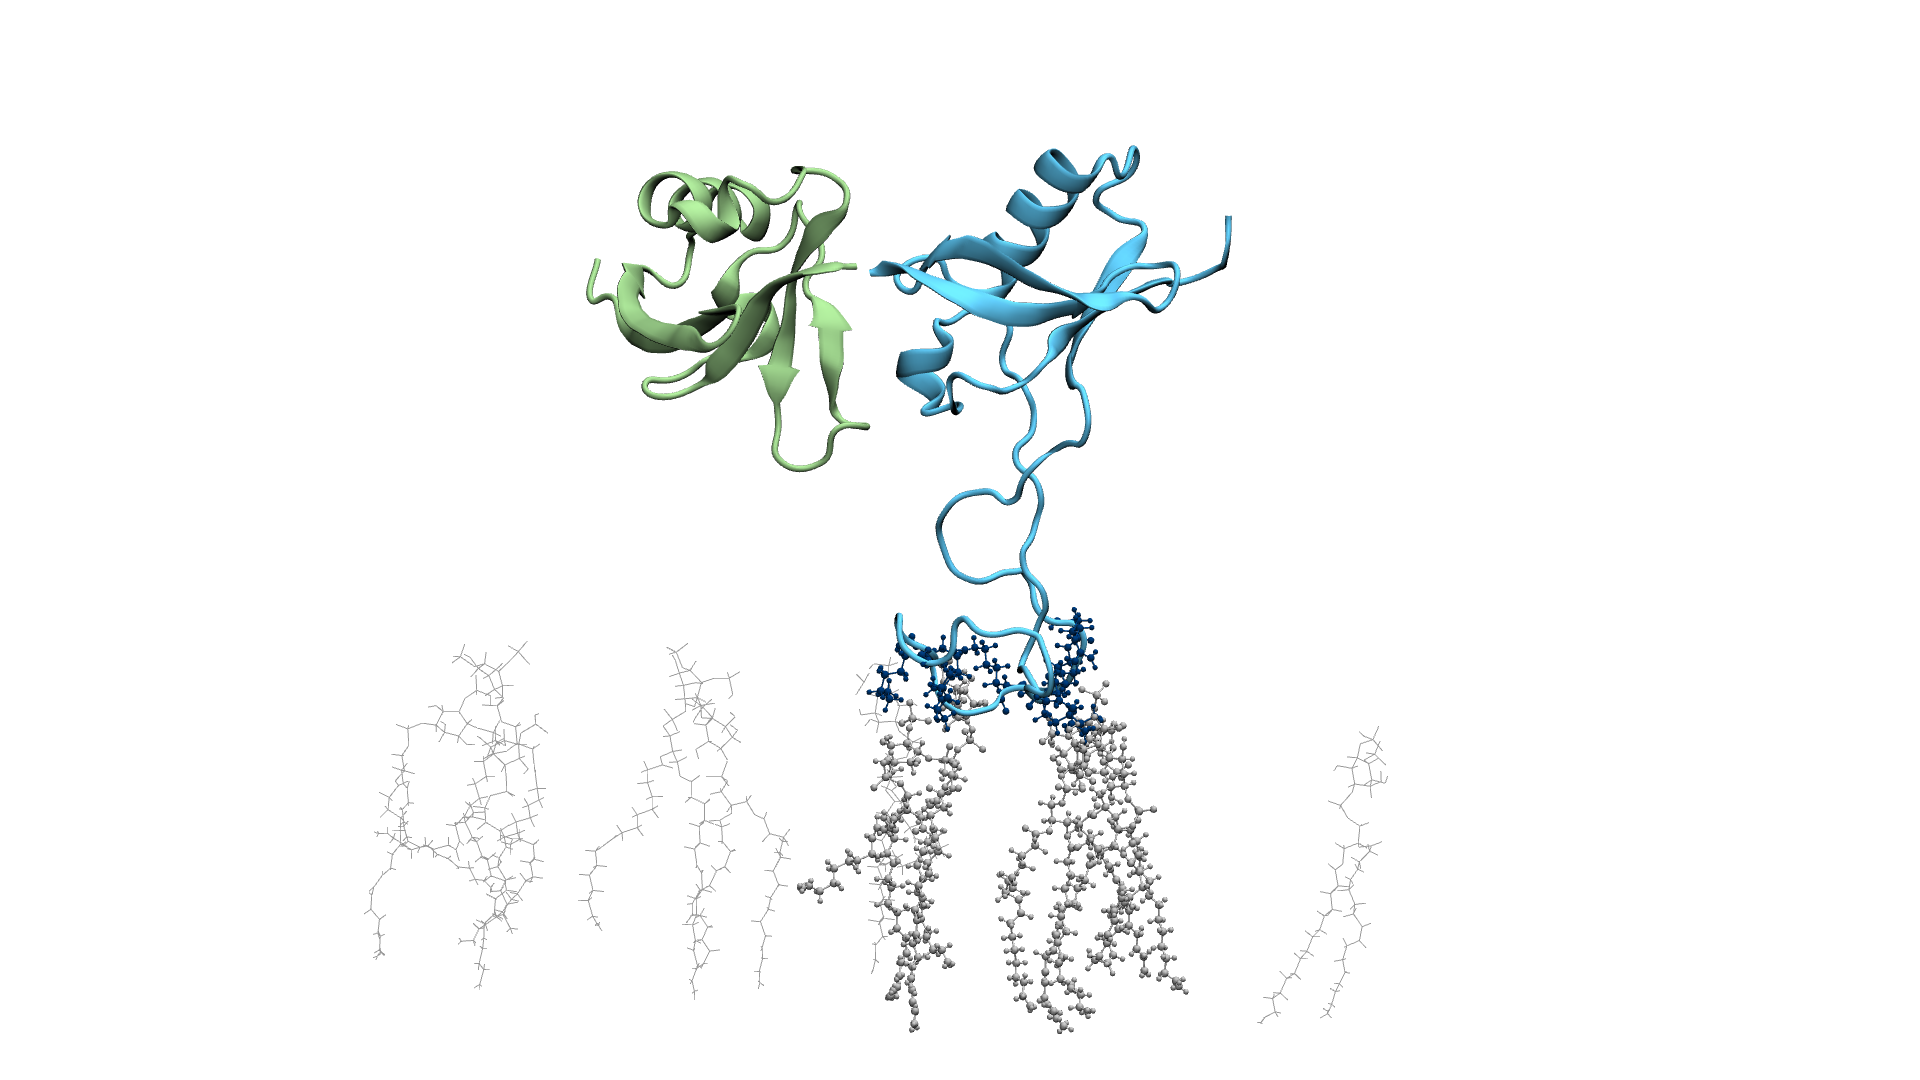
\includegraphics{./assets/vmd/f0f1/anchored.png}

}

}

\subcaption{\label{fig-f0f1-anchored}~}
\end{minipage}%
%
\begin{minipage}[t]{0.33\linewidth}

{\centering 

\raisebox{-\height}{

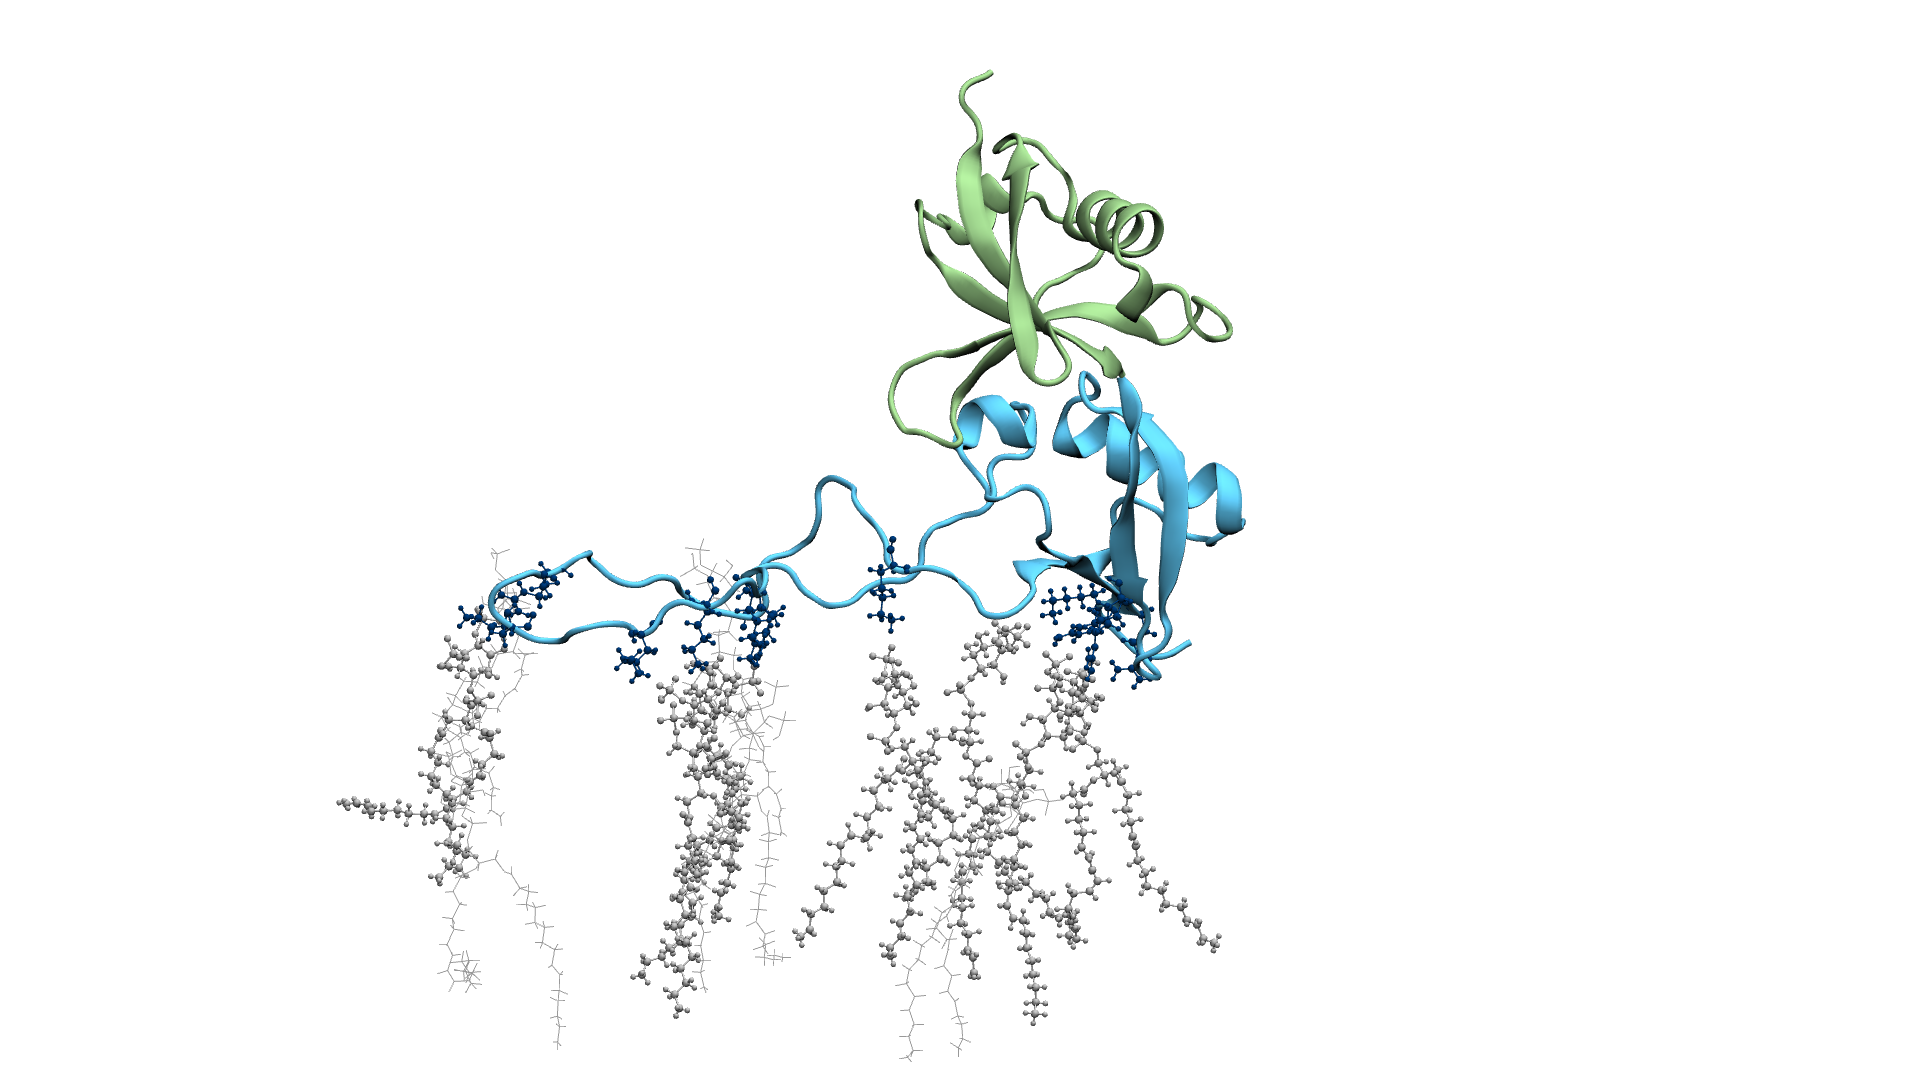
\includegraphics{./assets/vmd/f0f1/bound.png}

}

}

\subcaption{\label{fig-f0f1-bound}~}
\end{minipage}%
\newline
\begin{minipage}[t]{\linewidth}

{\centering 

\raisebox{-\height}{

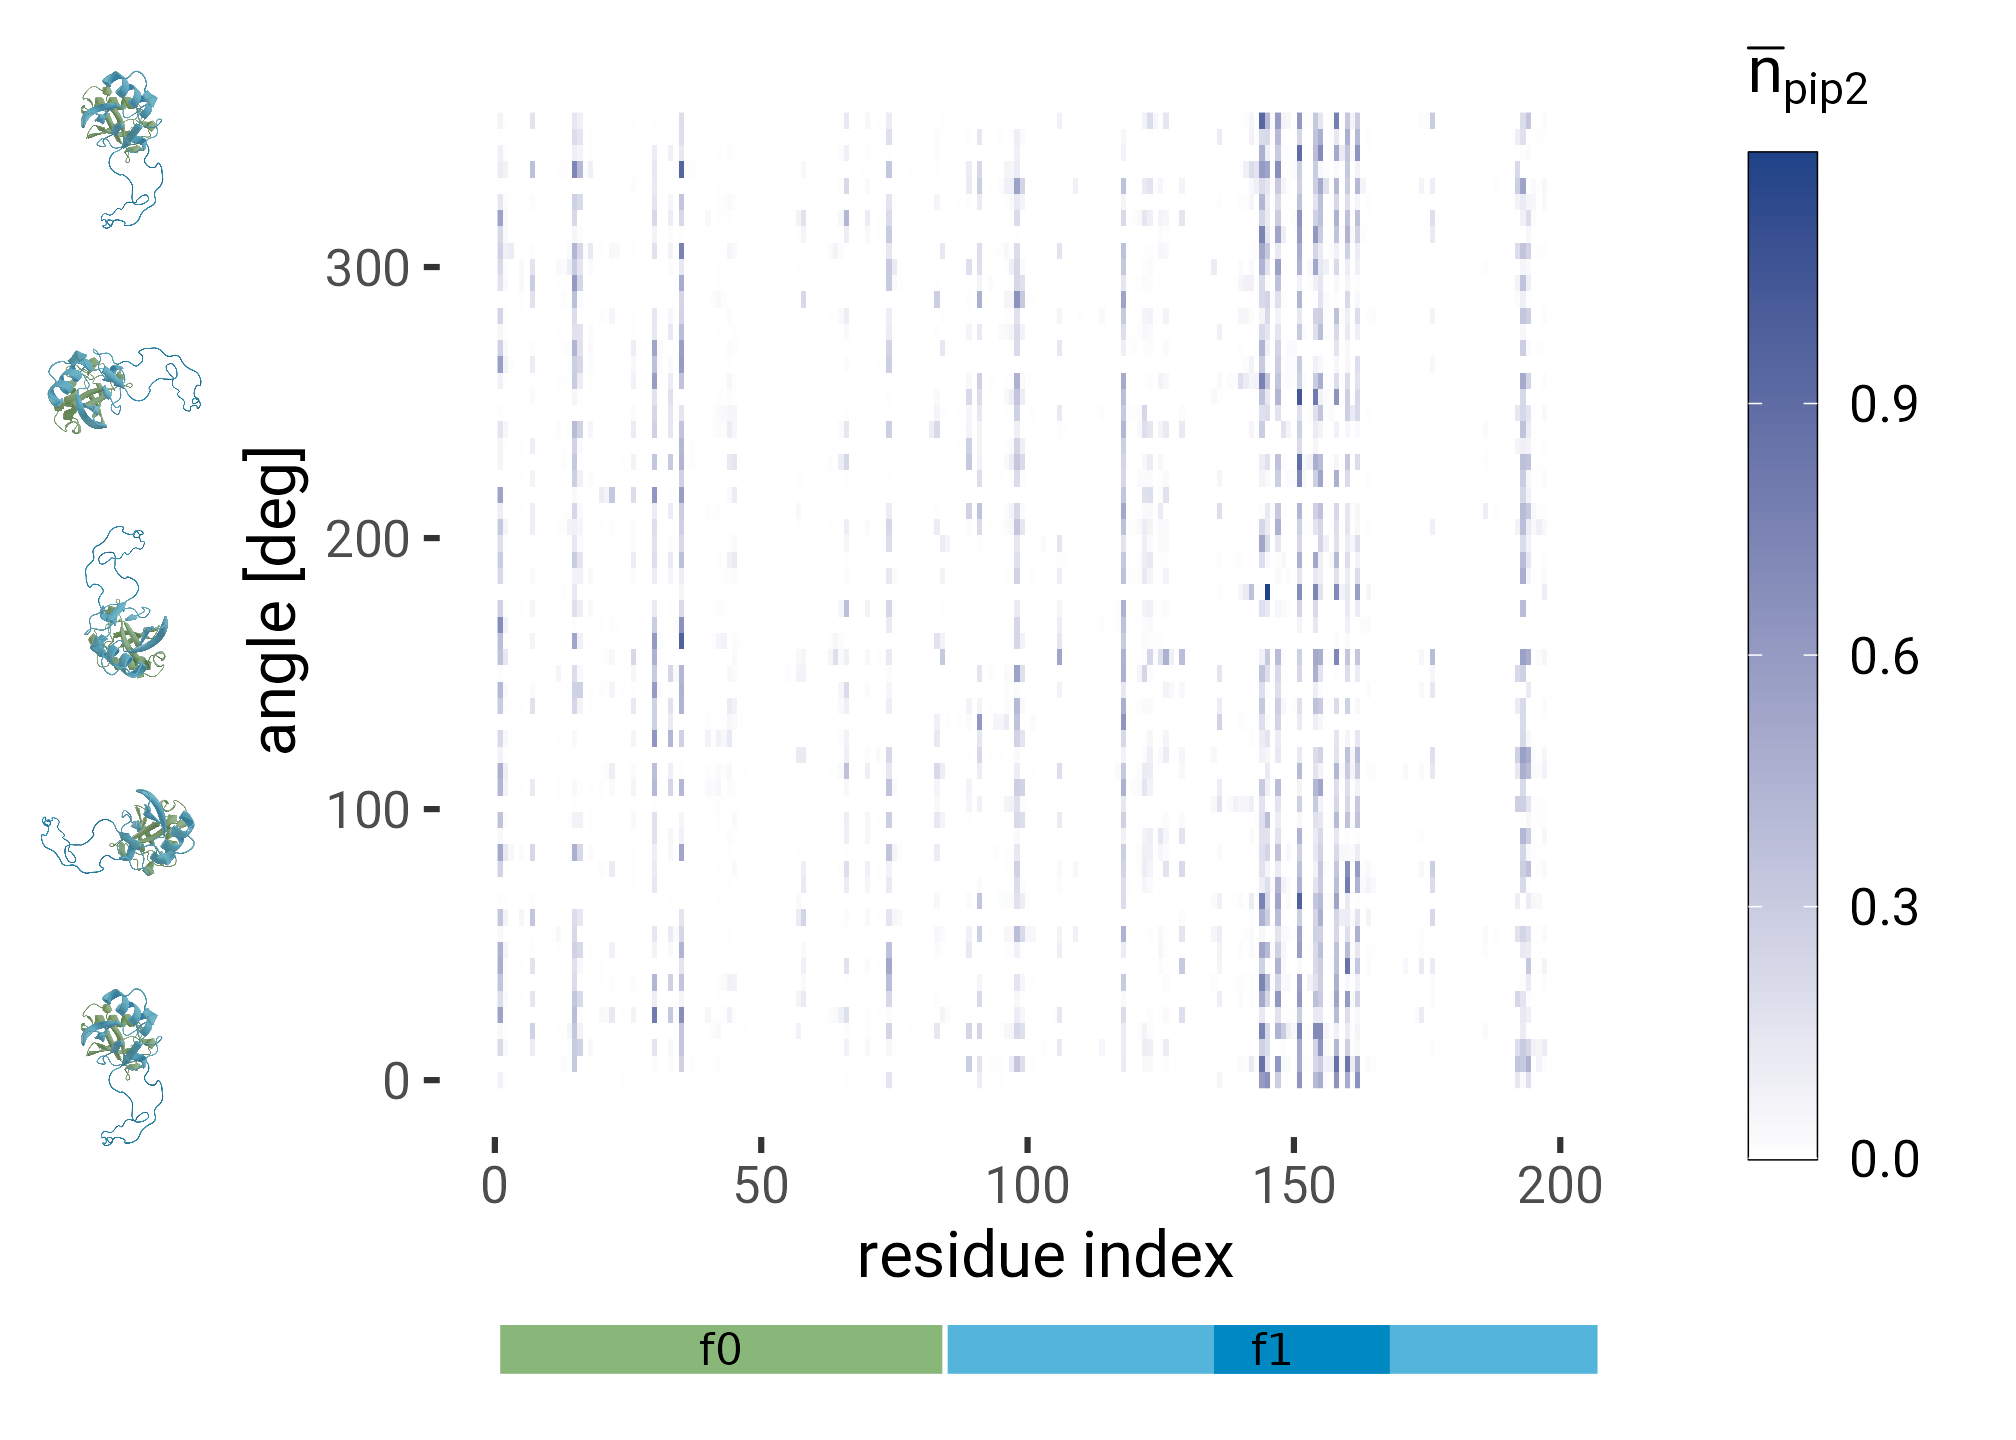
\includegraphics{./results/plots/f0f1-ri-angle-npip-1.png}

}

}

\subcaption{\label{fig-f0f1-ri-angle}~}
\end{minipage}%

\caption{\label{fig-loop-importance}Rotational sampling of F0-F1.
\textbf{a-c)} Snapshots from a simulation involving F0-F1 over a POPC
membrane containing 10\% PIP\textsubscript{2} in the upper leaflet. POPC
is not rendered and PIP\textsubscript{2} is shown as light grey stick
models that turn thicker for those molecules that are currently
interacting with residues of the protein. Those residues are then shown
as dark blue stick models. Once the F1 loop has made contact with the
membrane it can act as an anchor and facilitate further contacts,
ultimately pulling the protein onto the membrane. In order to test if
this interaction of the loop with the membrane is just the result of a
biased starting position with the loop already pointing downwards, we
sampled 60 different starting positions, rotated equally spaced around
the horizontal axis, with 6 replicates each. \textbf{d)} A heatmap
summarizing 358 simulations from the rotational sampling. Unfortunately
the number is not 360 because 2 trajectories were lost due to a hardware
failure. Each simulation is 200~ns long. Across all angles (y-axis) we
see that with very few exceptions the F1 loop (dark blue region on the
x-axis colorbar) is almost always involved in interactions 0° equates to
the loop pointing downwards towards the membrane. The heatmap color
represents the mean number of PIP\textsubscript{2} molecules that are in
close contact with the respective residue summarized over time and
replicates for that specific angle.}

\end{figure}

\begin{figure}

\begin{minipage}[t]{0.50\linewidth}

{\centering 

\raisebox{-\height}{

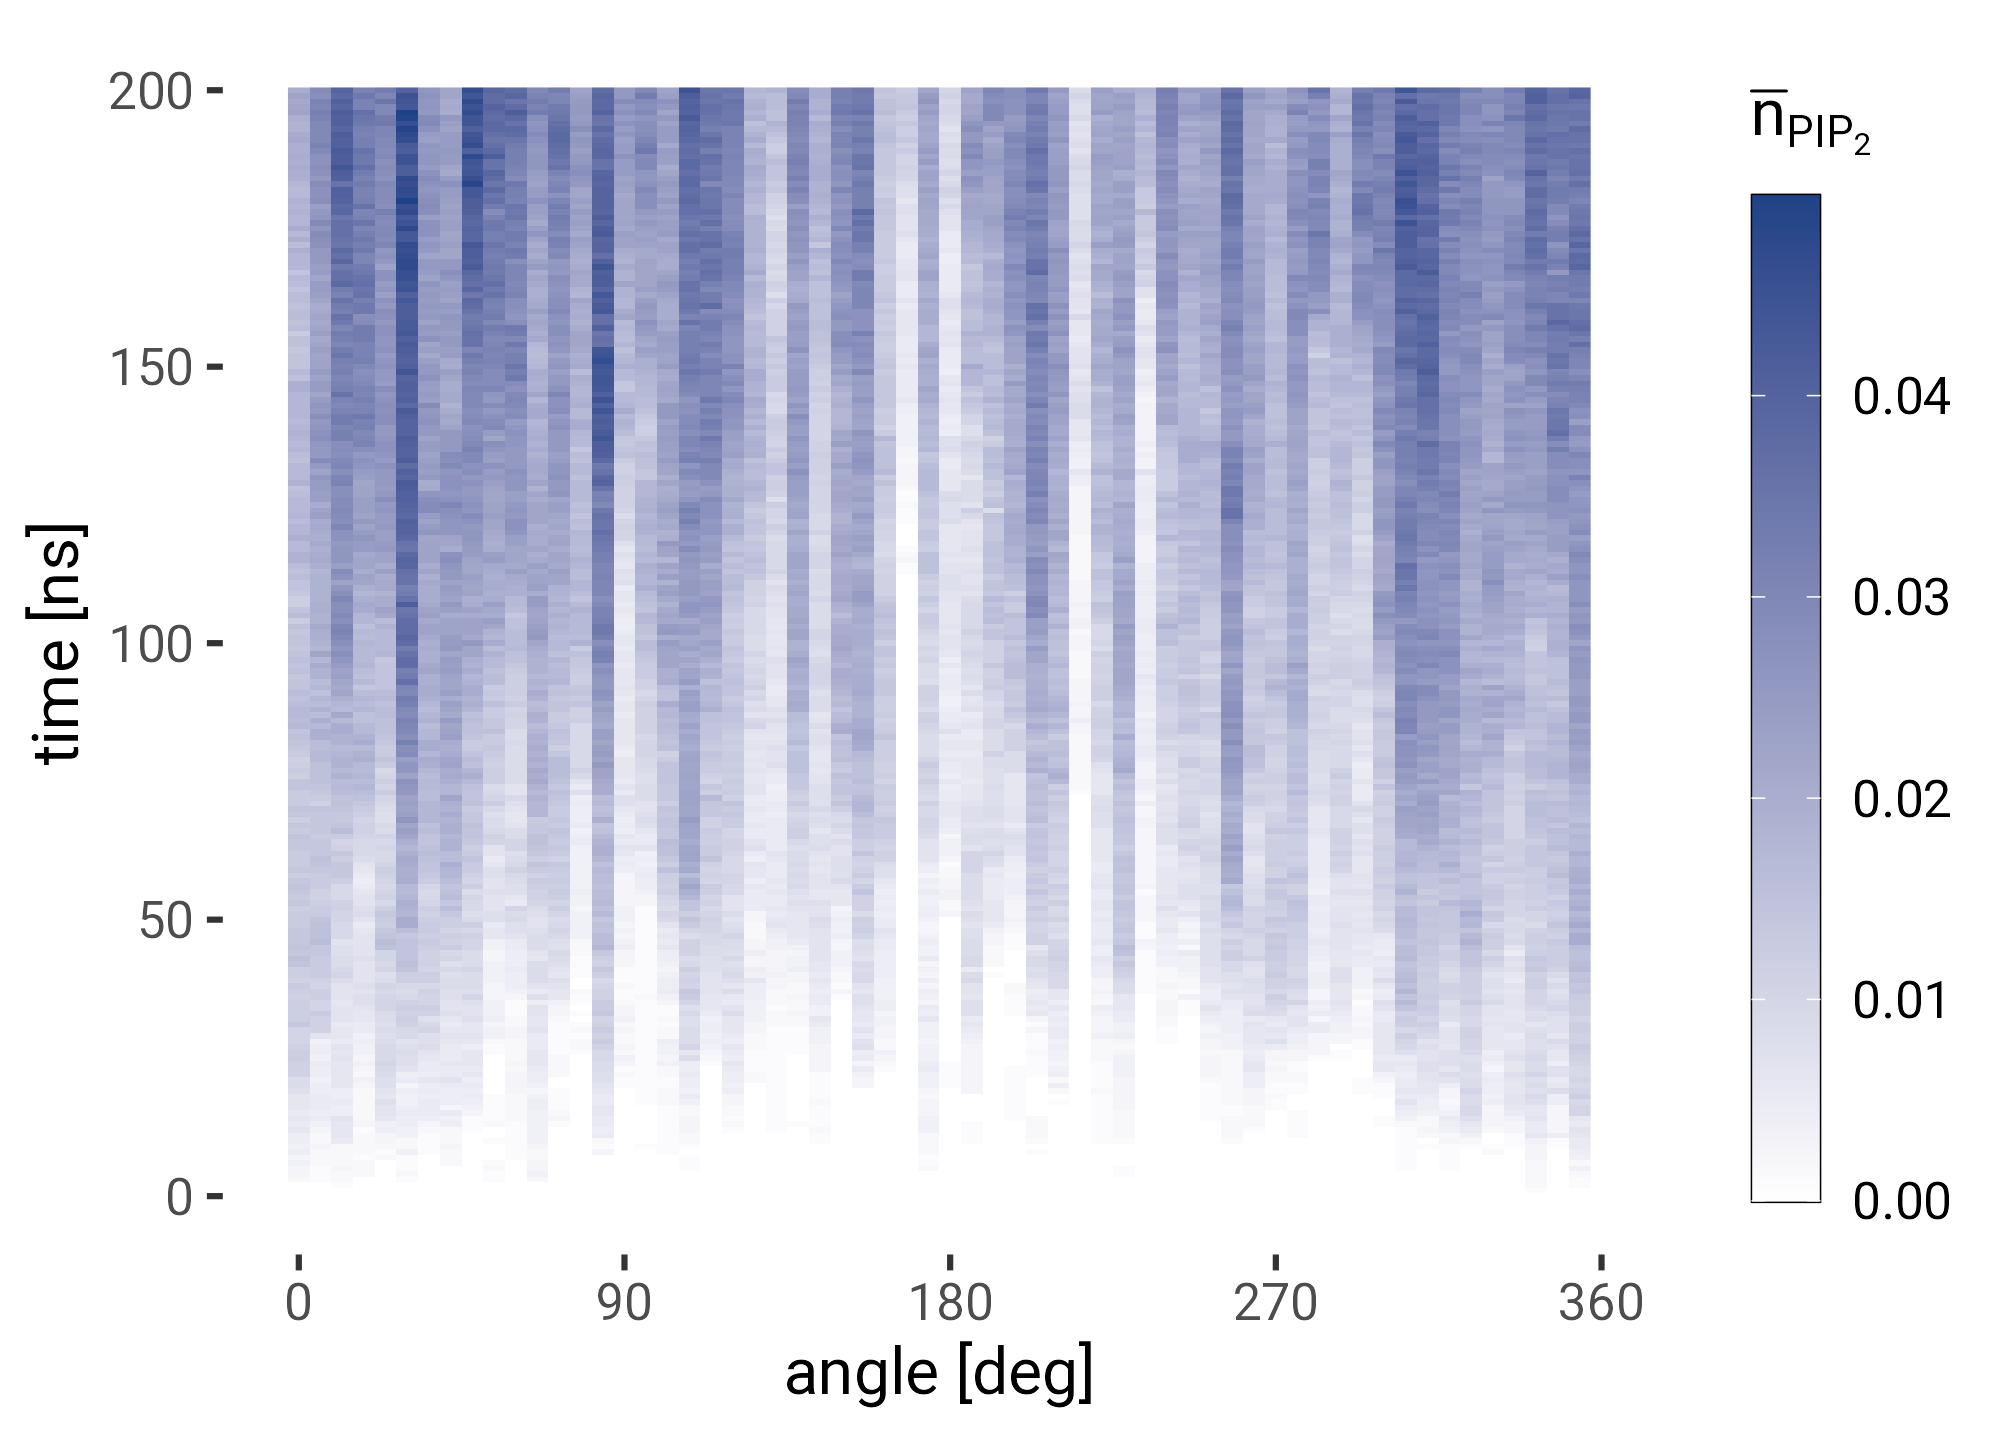
\includegraphics{./results/plots/f0f1-angle-frame-npip-1.png}

}

}

\subcaption{\label{fig-f0f1-angle-frame}~}
\end{minipage}%
%
\begin{minipage}[t]{0.50\linewidth}

{\centering 

\raisebox{-\height}{

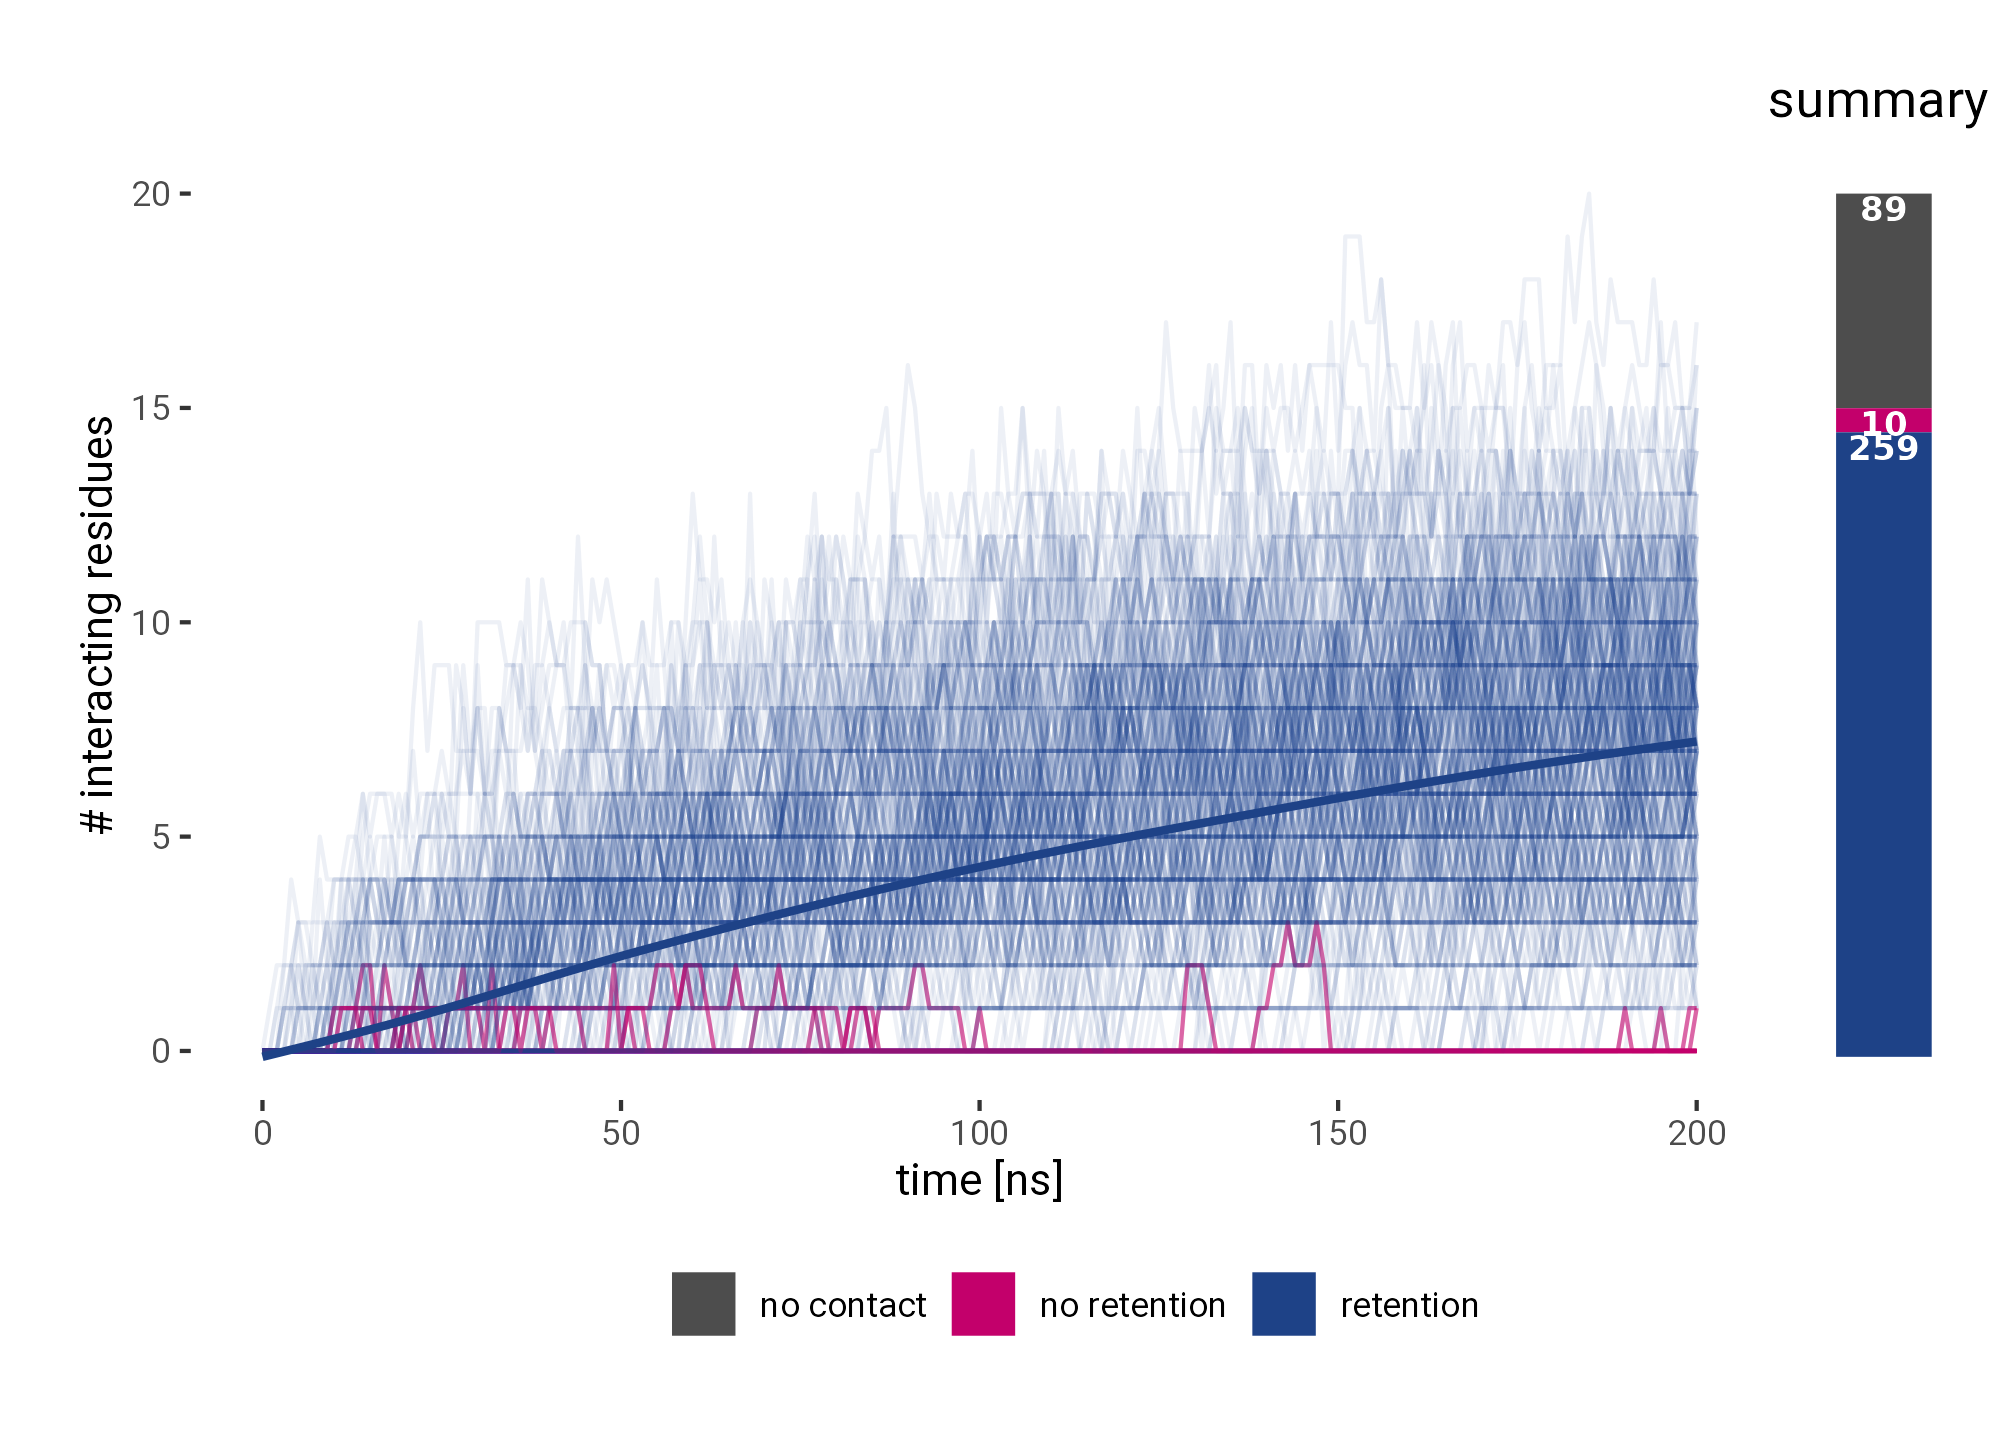
\includegraphics{./results/plots/f0f1-retention-1.png}

}

}

\subcaption{\label{fig-f0f1-retention}~}
\end{minipage}%

\caption{\label{fig-loop-importance}\textbf{a)} A heatmap of the time
evolution of the number of PIP\textsubscript{2} molecules at the
respective time and angle summarized over all residues and replicates.
Angles in which the loop is already favored towards the membrane tend to
make contact faster. Note that this trend is not simply because angles
favoring the loop would have been already closer to the membrane. The
protein was rotated in such a way that the respective closest residue
had the same distance to the membrane for the 0° and the 180° starting
positions. \textbf{b)} A time evolution of the simulations shows the
number of interacting residues gradually increasing as the anchored
protein gets pulled closer towards the membrane by the forming
interactions. Only in 10 simulations (out of 269 simulations that had at
least one contact) did the protein leave the membrane again within the
200~ns long timeframe. This never occurred after more than 3 residues
had already made contact.}

\end{figure}

\begin{figure}

\begin{minipage}[t]{\linewidth}

{\centering 

\raisebox{-\height}{

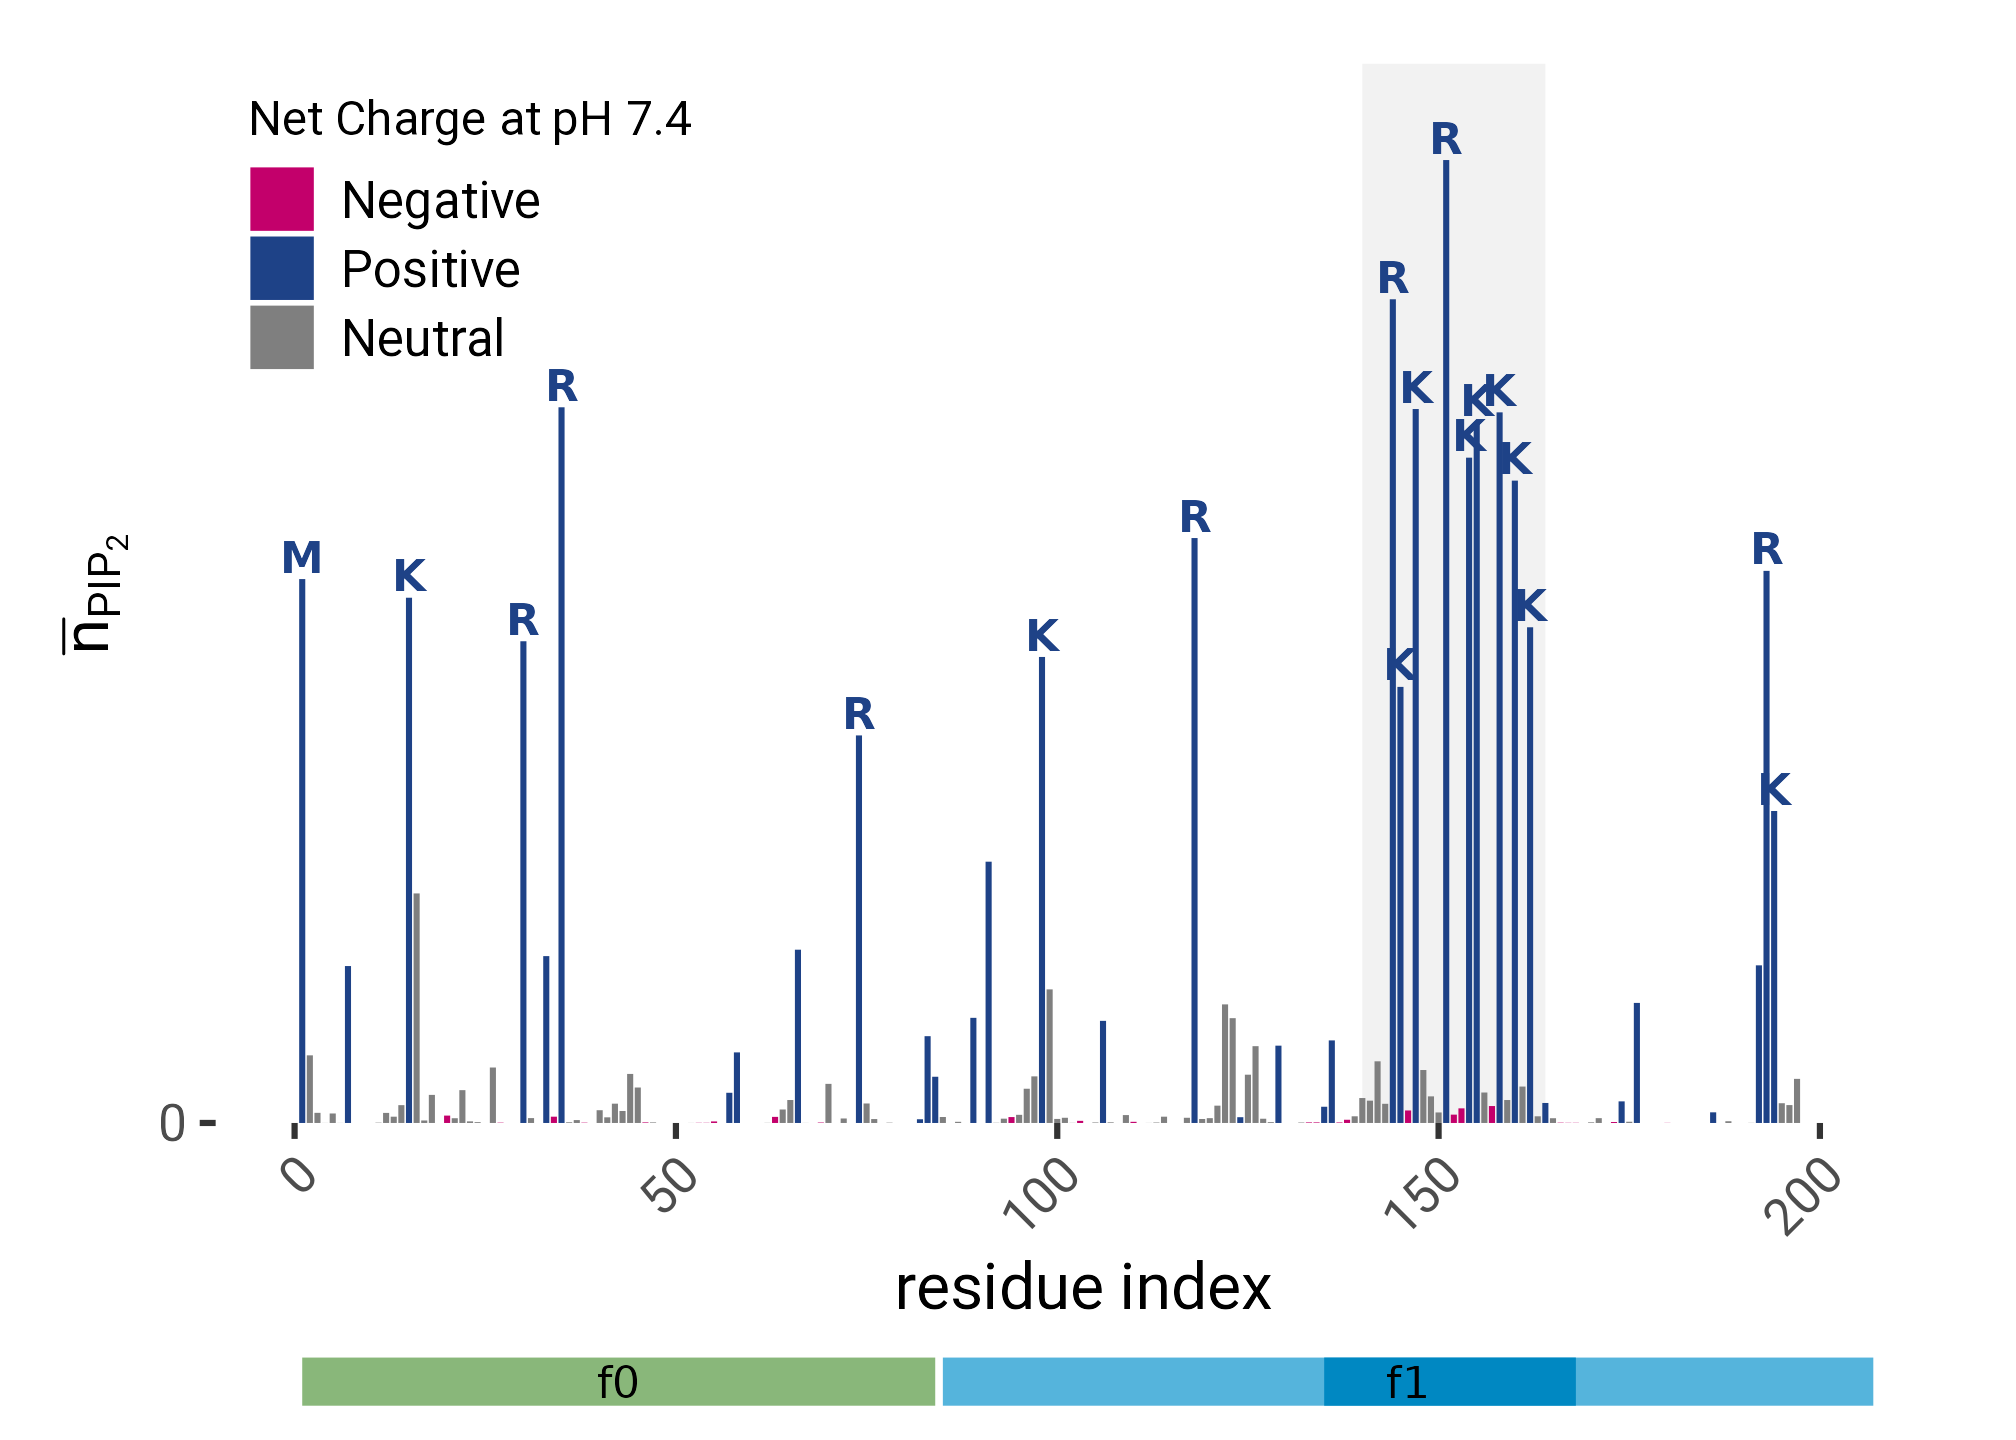
\includegraphics{./results/plots/f0f1-ri-npip-1.png}

}

}

\subcaption{\label{fig-f0f1-ri-npip}~}
\end{minipage}%
\newline
\begin{minipage}[t]{\linewidth}

{\centering 

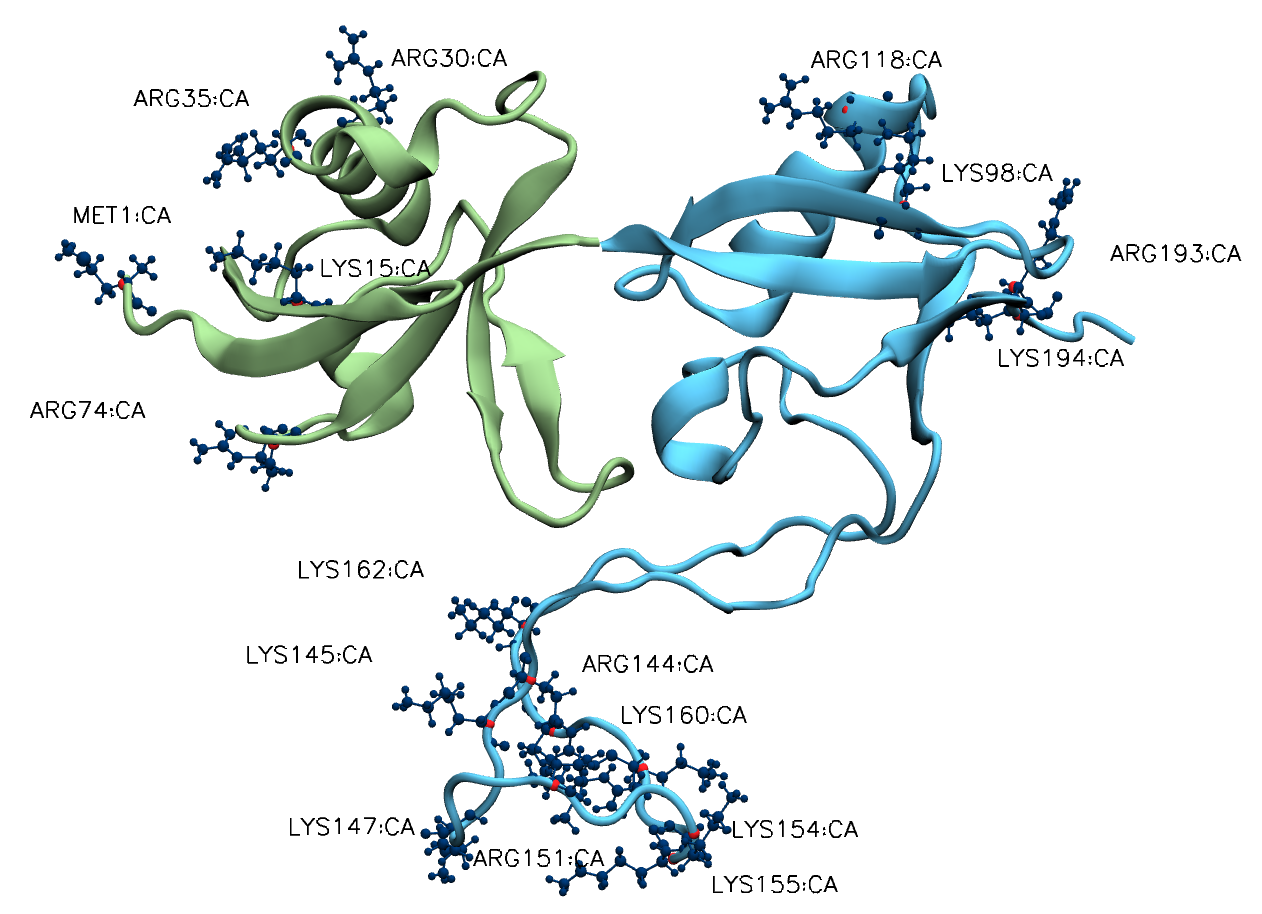
\includegraphics{./assets/vmd/f0f1/residues.png}

}

\subcaption{\label{fig-f1f1-residues}~}
\end{minipage}%

\caption{\label{fig-f0f1-residues}PIP\textsubscript{2}-interacting
residues of F0-F1. \textbf{a)} The Mean interaction scores of the
individual residues across all simulations that made contact with the
membrane. Color represents the isoelectric point of the amino acid in
isolation (blue = basic, magenta = acidic). A number of very prominent
lysines can be observed, as well as a cluster of residues belonging to
the F1 loop. The most prominent residues are highlighted in \textbf{b)}.
(For the print version it is just a placeholder image. The video is
available in the web-version
(\url{https://hits-mbm-dev.github.io/paper-talin-loop}) or here:
\url{https://youtu.be/s5yya0XeNTA}).}

\end{figure}

\hypertarget{the-f1-loop-can-facilitate-further-contacts}{%
\subsection{The F1 loop can facilitate further
contacts}\label{the-f1-loop-can-facilitate-further-contacts}}

We chose a representative conformation from the rotational sampling as a
starting point for force-probe simulations of F0-F1 perpendicular to the
membrane to test the strength of the interaction
(Figure~\ref{fig-f0f1-vert-pull-vmd}). An exemplary render of one of the
simulations can be seen in Figure~\ref{fig-f0f1-pull-run-1}. Pulling
F0-F1 off the membrane requires peak forces of 100--120~pN, during which
the interacting residues only very gradually loose contact
(Figure~\ref{fig-f0f1-vert-pull}). This highlights the strong anchoring
capabilities of the F1 loop. As seen in
Figure~\ref{fig-f0f1-vert-pull-contacts}, during pulling residues not
belonging to the F1 loop loose contact first, while the loop stays
attached. The F1 loop works in conjunction with the F0 subdomain (see
Figure~\ref{fig-f0f1-vert-pull-residues}). Their high flexibility allows
them to remain in contact with the membrane over large distances, which
would allow for a spring-like re-establishing of more contacts should
the force be alleviated.

\begin{figure}

\begin{minipage}[t]{0.61\linewidth}

{\centering 

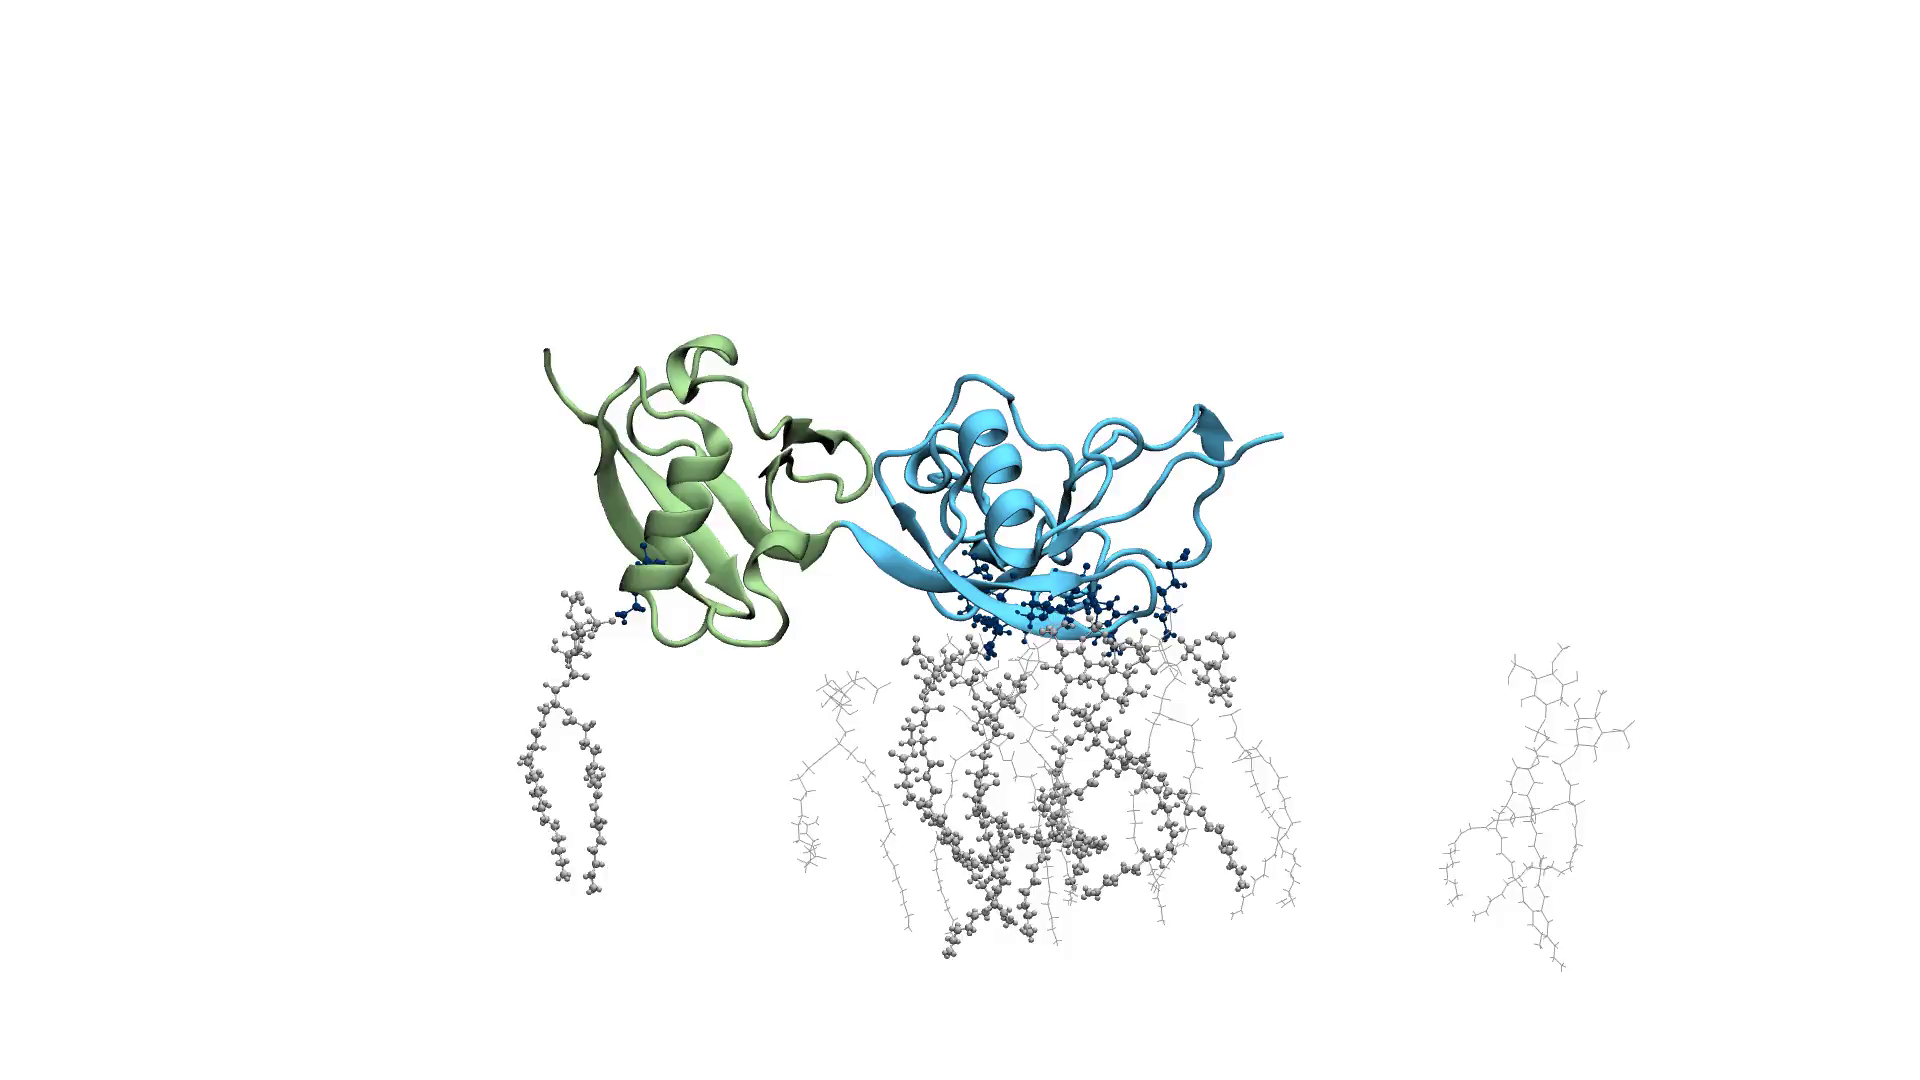
\includegraphics{./assets/vmd/f0f1-pulling/f0f1-pull-start.png}
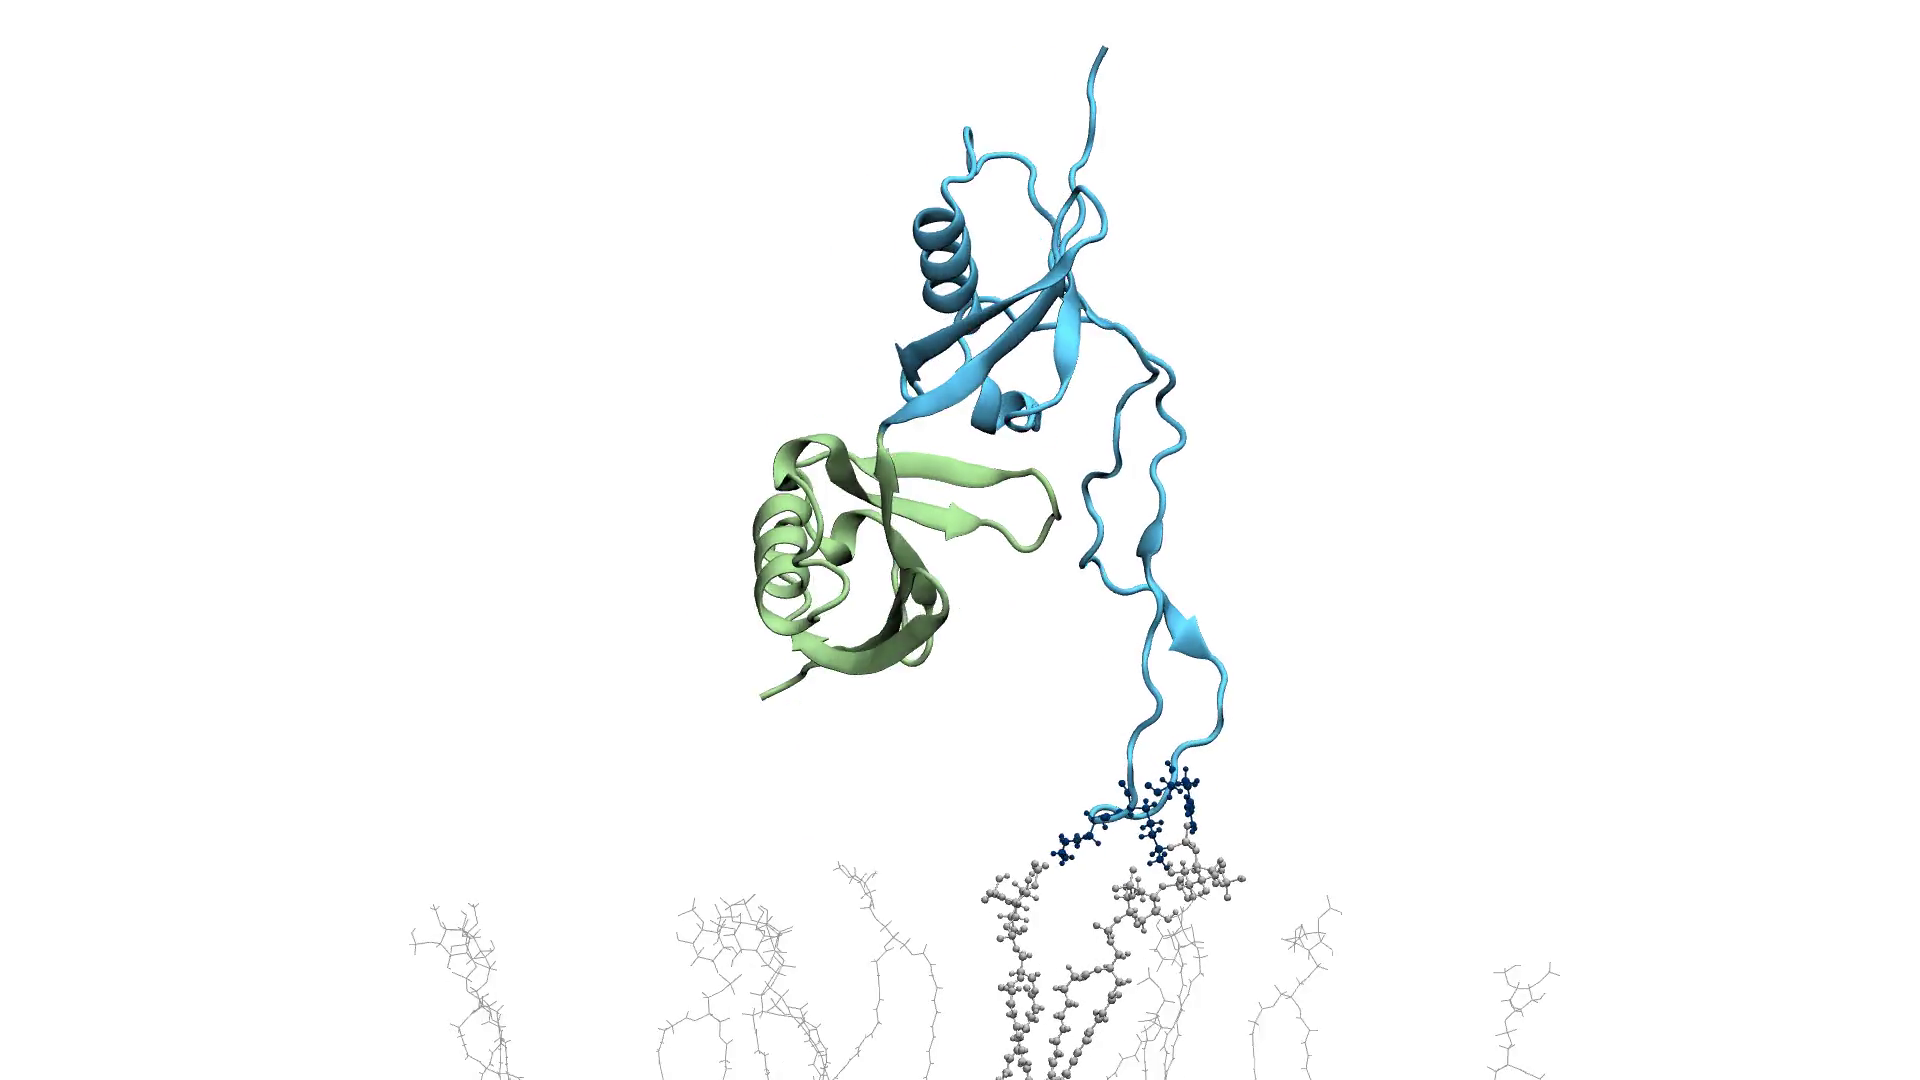
\includegraphics{./assets/vmd/f0f1-pulling/f0f1-pull-end.png}

}

\subcaption{\label{fig-f0f1-pull-run-1}~}
\end{minipage}%
%
\begin{minipage}[t]{0.39\linewidth}

{\centering 

\raisebox{-\height}{

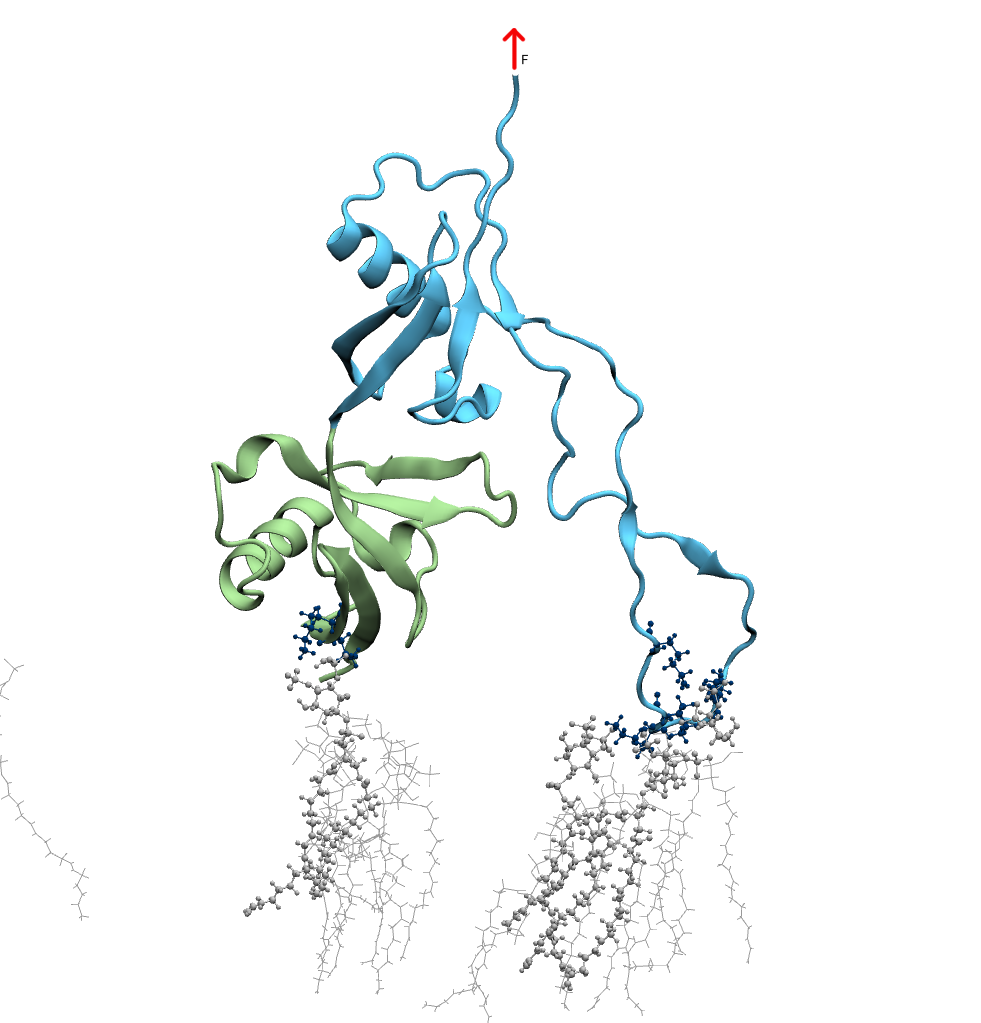
\includegraphics{./assets/vmd/f0f1-pulling/vert-pull.png}

}

}

\subcaption{\label{fig-f0f1-vert-pull-vmd}~}
\end{minipage}%
\newline
\begin{minipage}[t]{0.50\linewidth}

{\centering 

\raisebox{-\height}{

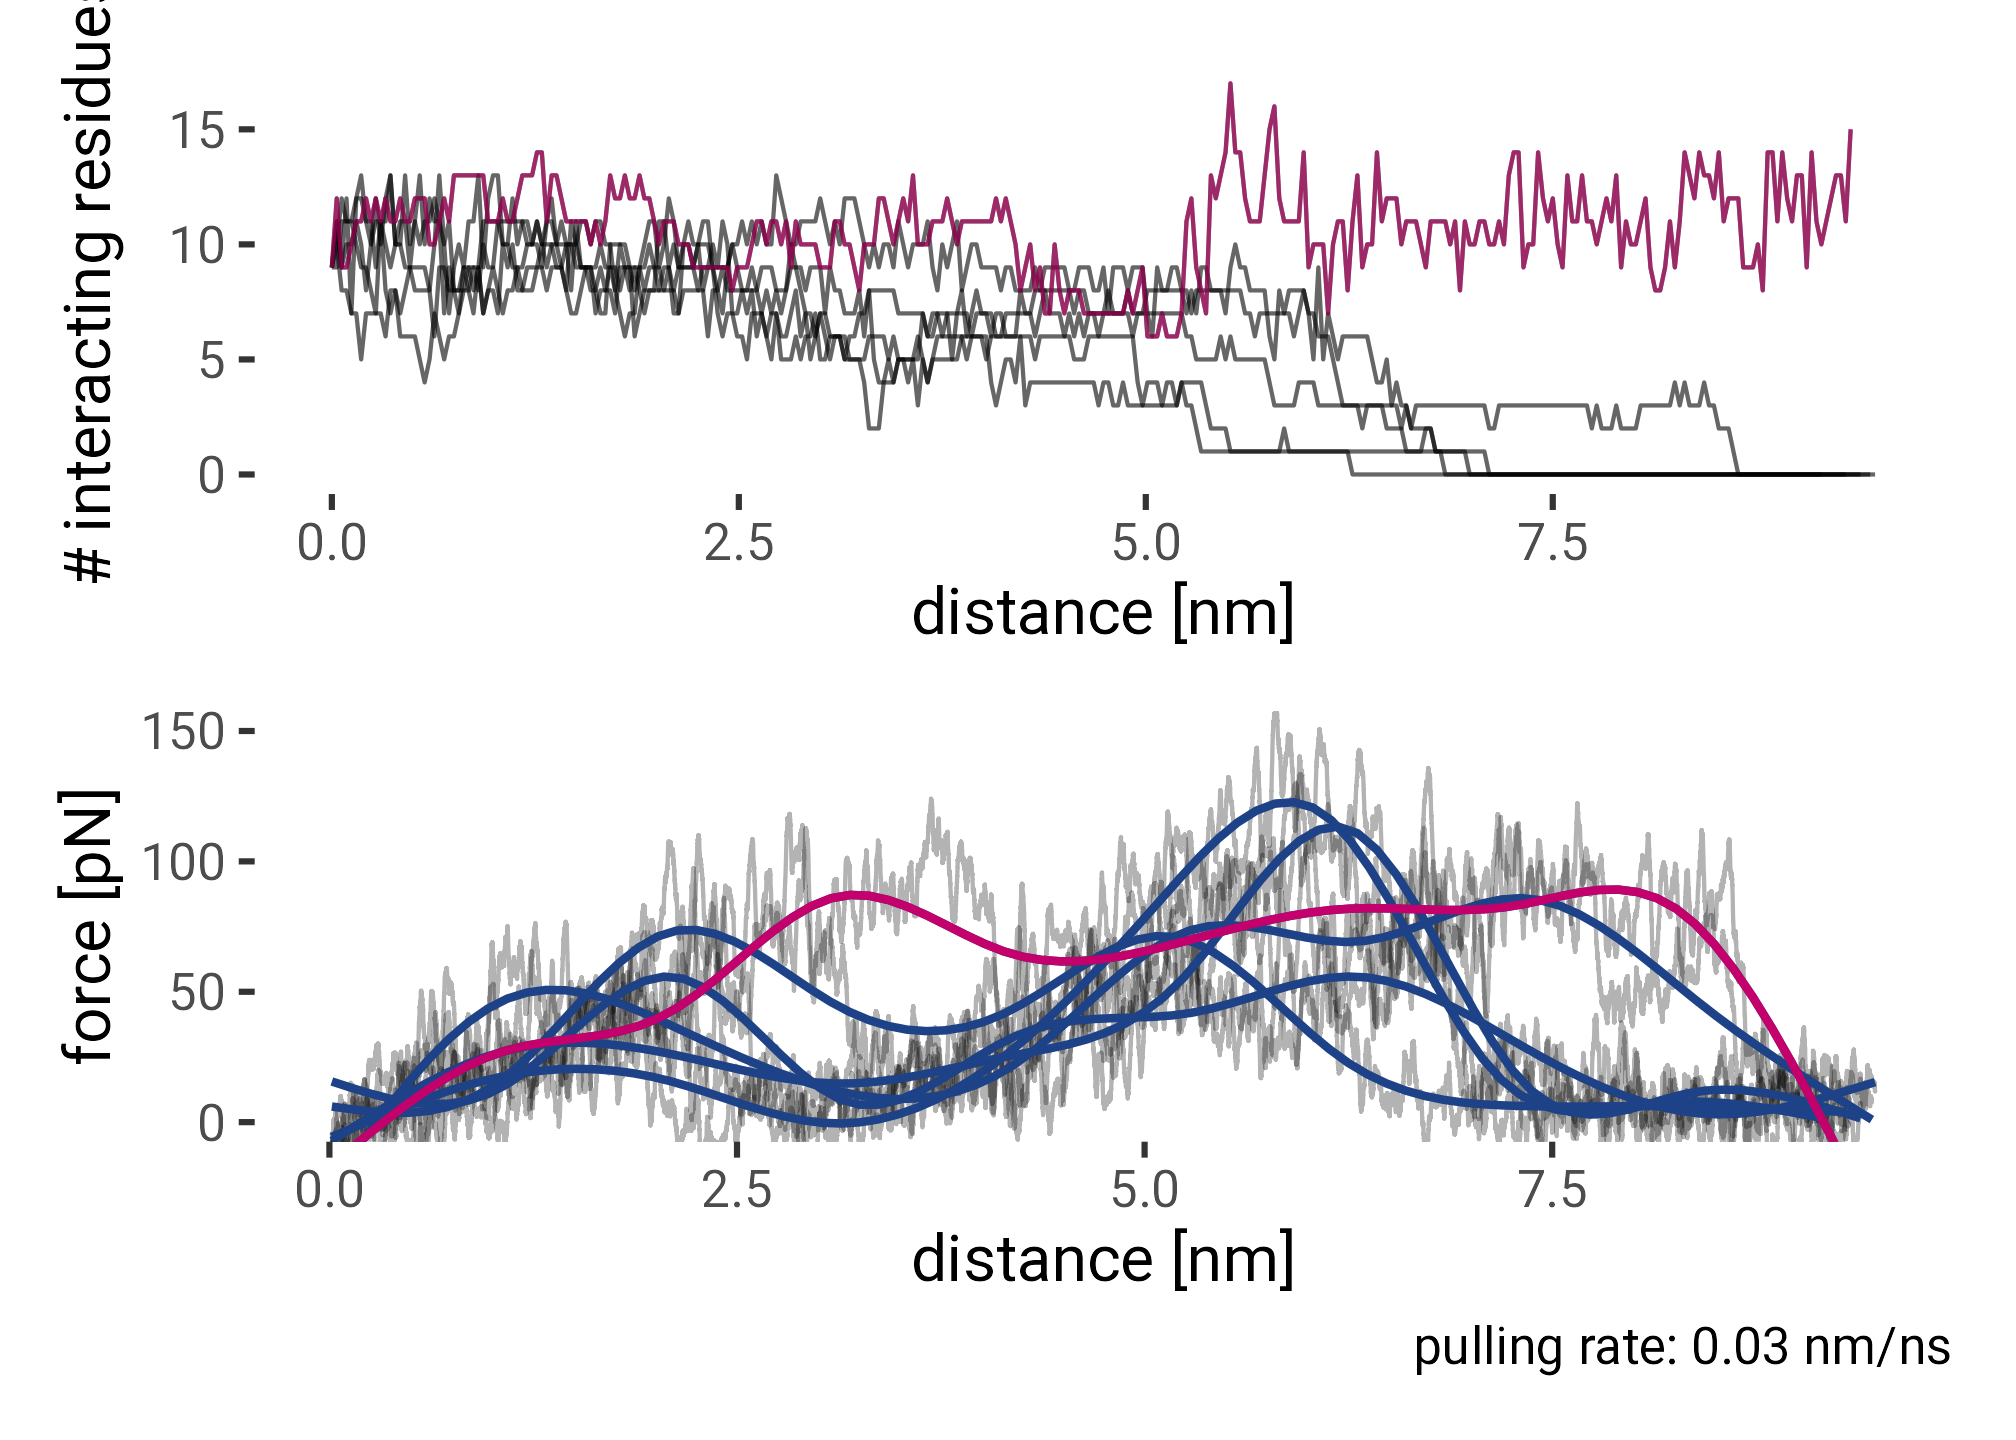
\includegraphics{./results/plots/f0f1-vert-pull-1.png}

}

}

\subcaption{\label{fig-f0f1-vert-pull}~}
\end{minipage}%
%
\begin{minipage}[t]{0.50\linewidth}

{\centering 

\raisebox{-\height}{

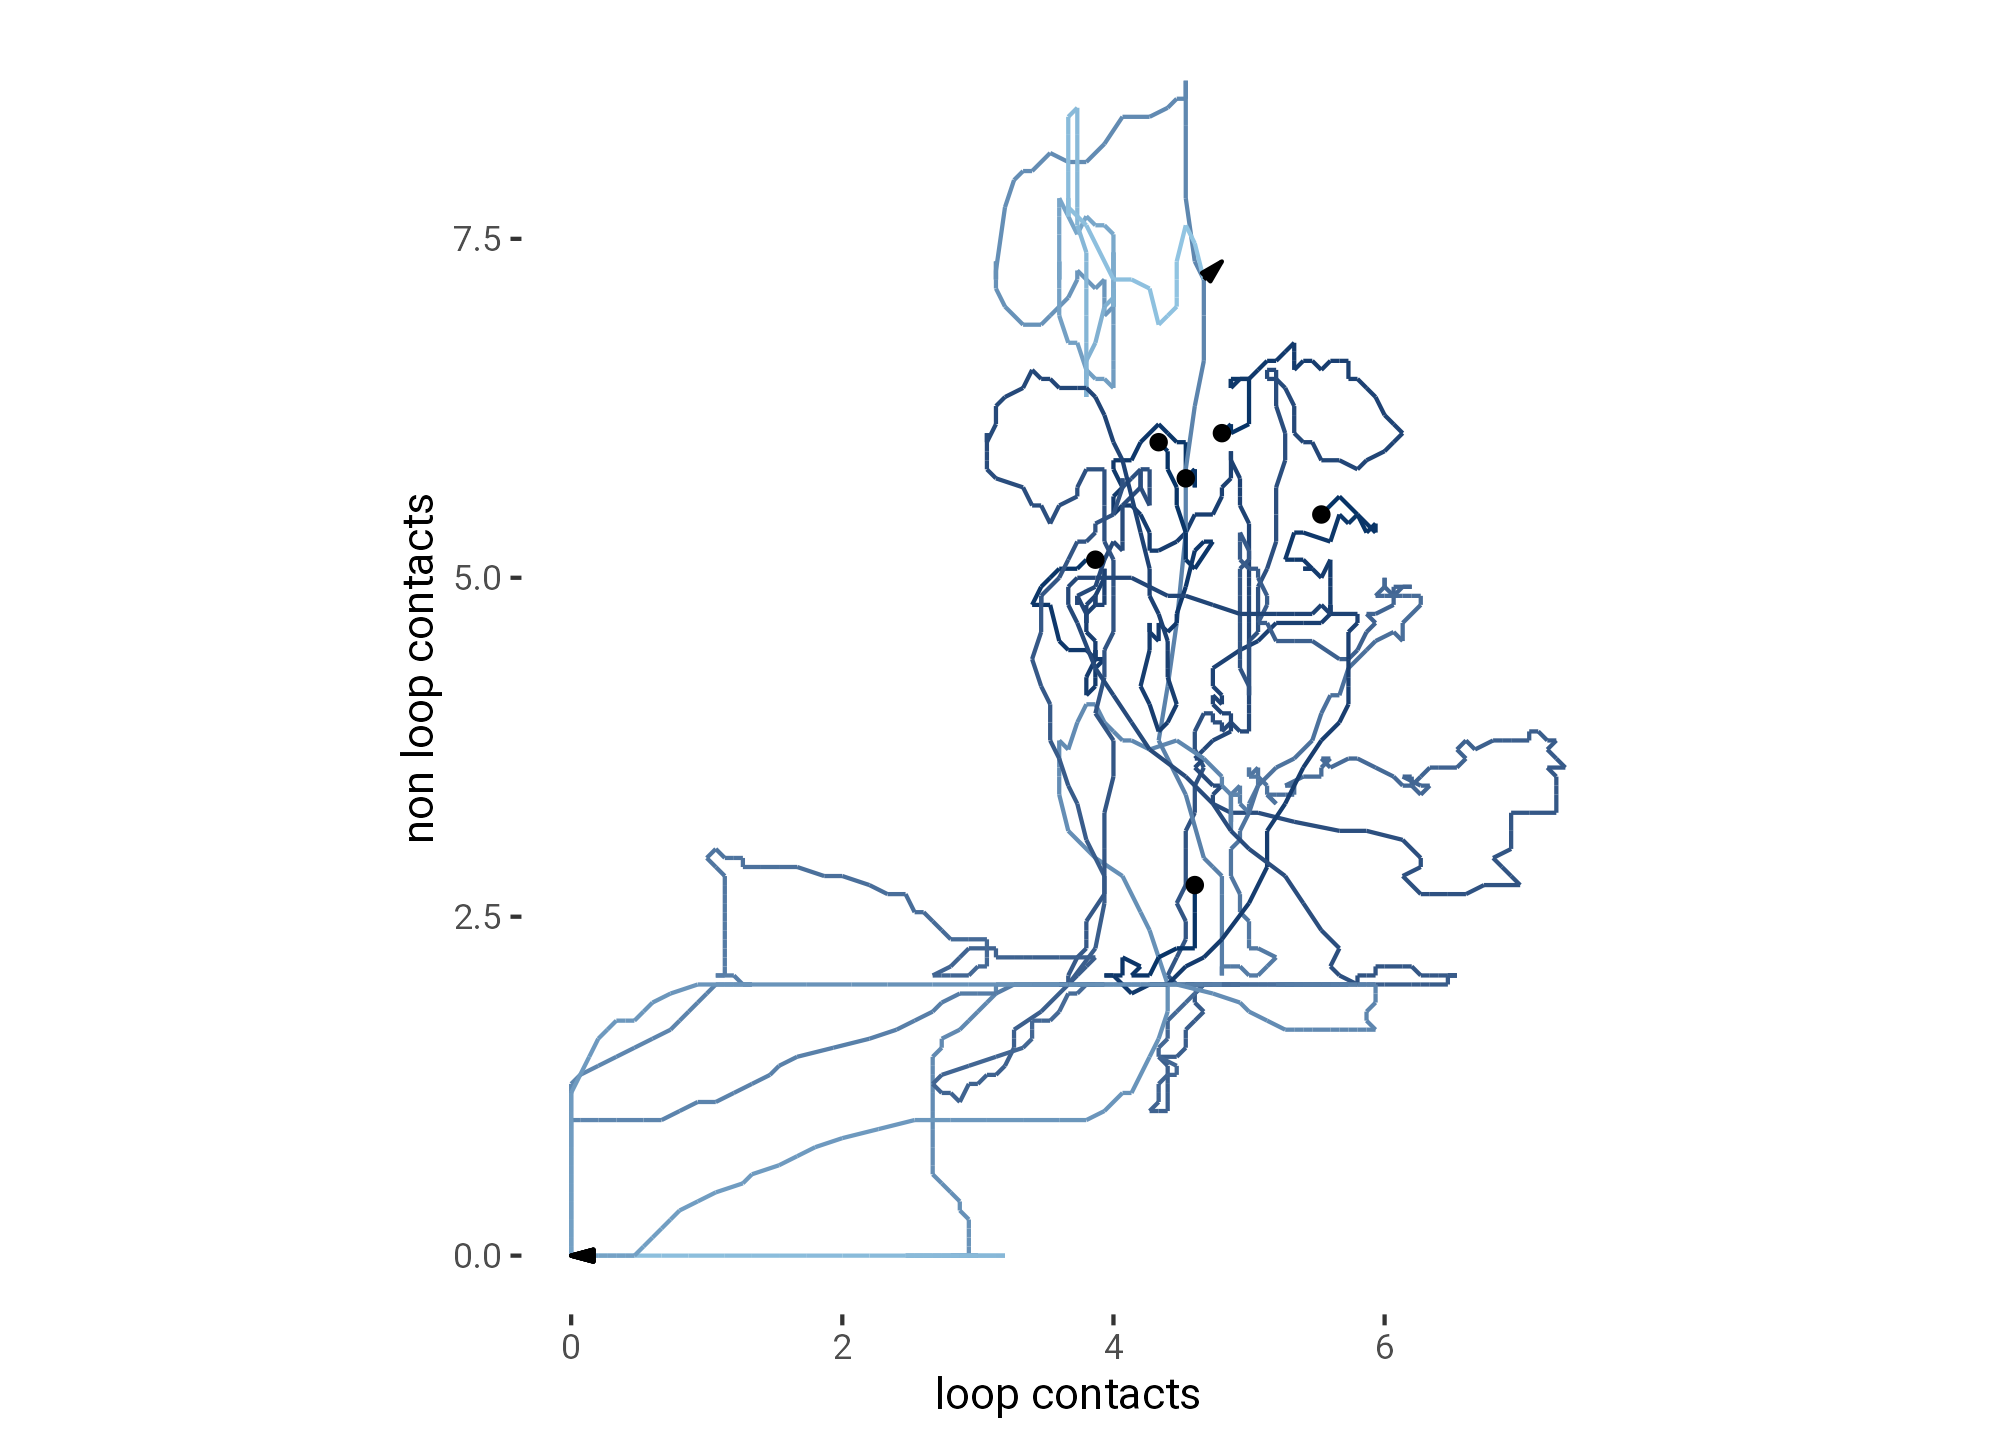
\includegraphics{./results/plots/f0f1-vert-pull-contacts-time-1.png}

}

}

\subcaption{\label{fig-f0f1-vert-pull-contacts}~}
\end{minipage}%

\caption{\label{fig-vert-pull}Vertical Pulling of F0-F1. \textbf{a)} A
representative render of one of 6 force-probe MD simulations pulling
F0-F1 off the membrane (For the print version it is just a placeholder
image. The video is available in the web-version
(\url{https://hits-mbm-dev.github.io/paper-talin-loop} or here:
\url{https://youtu.be/-eZ2orx7QRE}). It starts from a snapshot of F0-F1
in its bound conformation taken from the rotational sampling
(Figure~\ref{fig-loop-importance}) and gets pulled upwards from its
C-terminus. The direction of force is shown in the snapshot \textbf{b)}.
\textbf{c)} As F0-F1 gets pulled at a constant rate of 0.03~nm/ns we
observe the time evolution of the force (bottom panel) and the number of
interacting residues (top panel). The number of interacting residues
goes down very gradually, as the high flexibility of loop allows the
residues to remain in contact even as the distance increases. Replicate
4 is highlighted in magenta, as in this run the interactions were so so
strong that a total of 3 molecules of PIP\textsubscript{2} were pulled
out of the membrane (1 by F0 and 2 by the F1 loop). A snapshot of this
can be seen in Figure~\ref{fig-f0f1-vert-pull-run4}. \textbf{d)} The
time evolution of the number of contacts for resides belonging to the F1
loop and other residues shows how initially other residues loose contact
until eventually the loop looses contacts as well. Lighter shades of
blue correspond to a later time in the simulation. Black dots mark the
starting positions. The longest remaining non-loop contacts belong to
the N-terminus of F0 (for which \textbf{b} is also a representative
snapshot), with the exception of replicate 4, as explained in
\textbf{c}.}

\end{figure}

Simulations with the full-length FERM domain show that with the loop as
an initial membrane contact, known PIP\textsubscript{2} binding sites
can also be established
(Figure~\ref{fig-ferm-ri-npip}, Figure~\ref{fig-ferm-memb-system}). The
highlighted residues include K272 of F2 and K316, K324, E342, and K343
of F3, which have been shown to be crucial for the membrane interaction
of Talin and subsequent integrin activation by Chinthalapudi et al.
(20).

\begin{figure}

\begin{minipage}[t]{\linewidth}

{\centering 

\raisebox{-\height}{

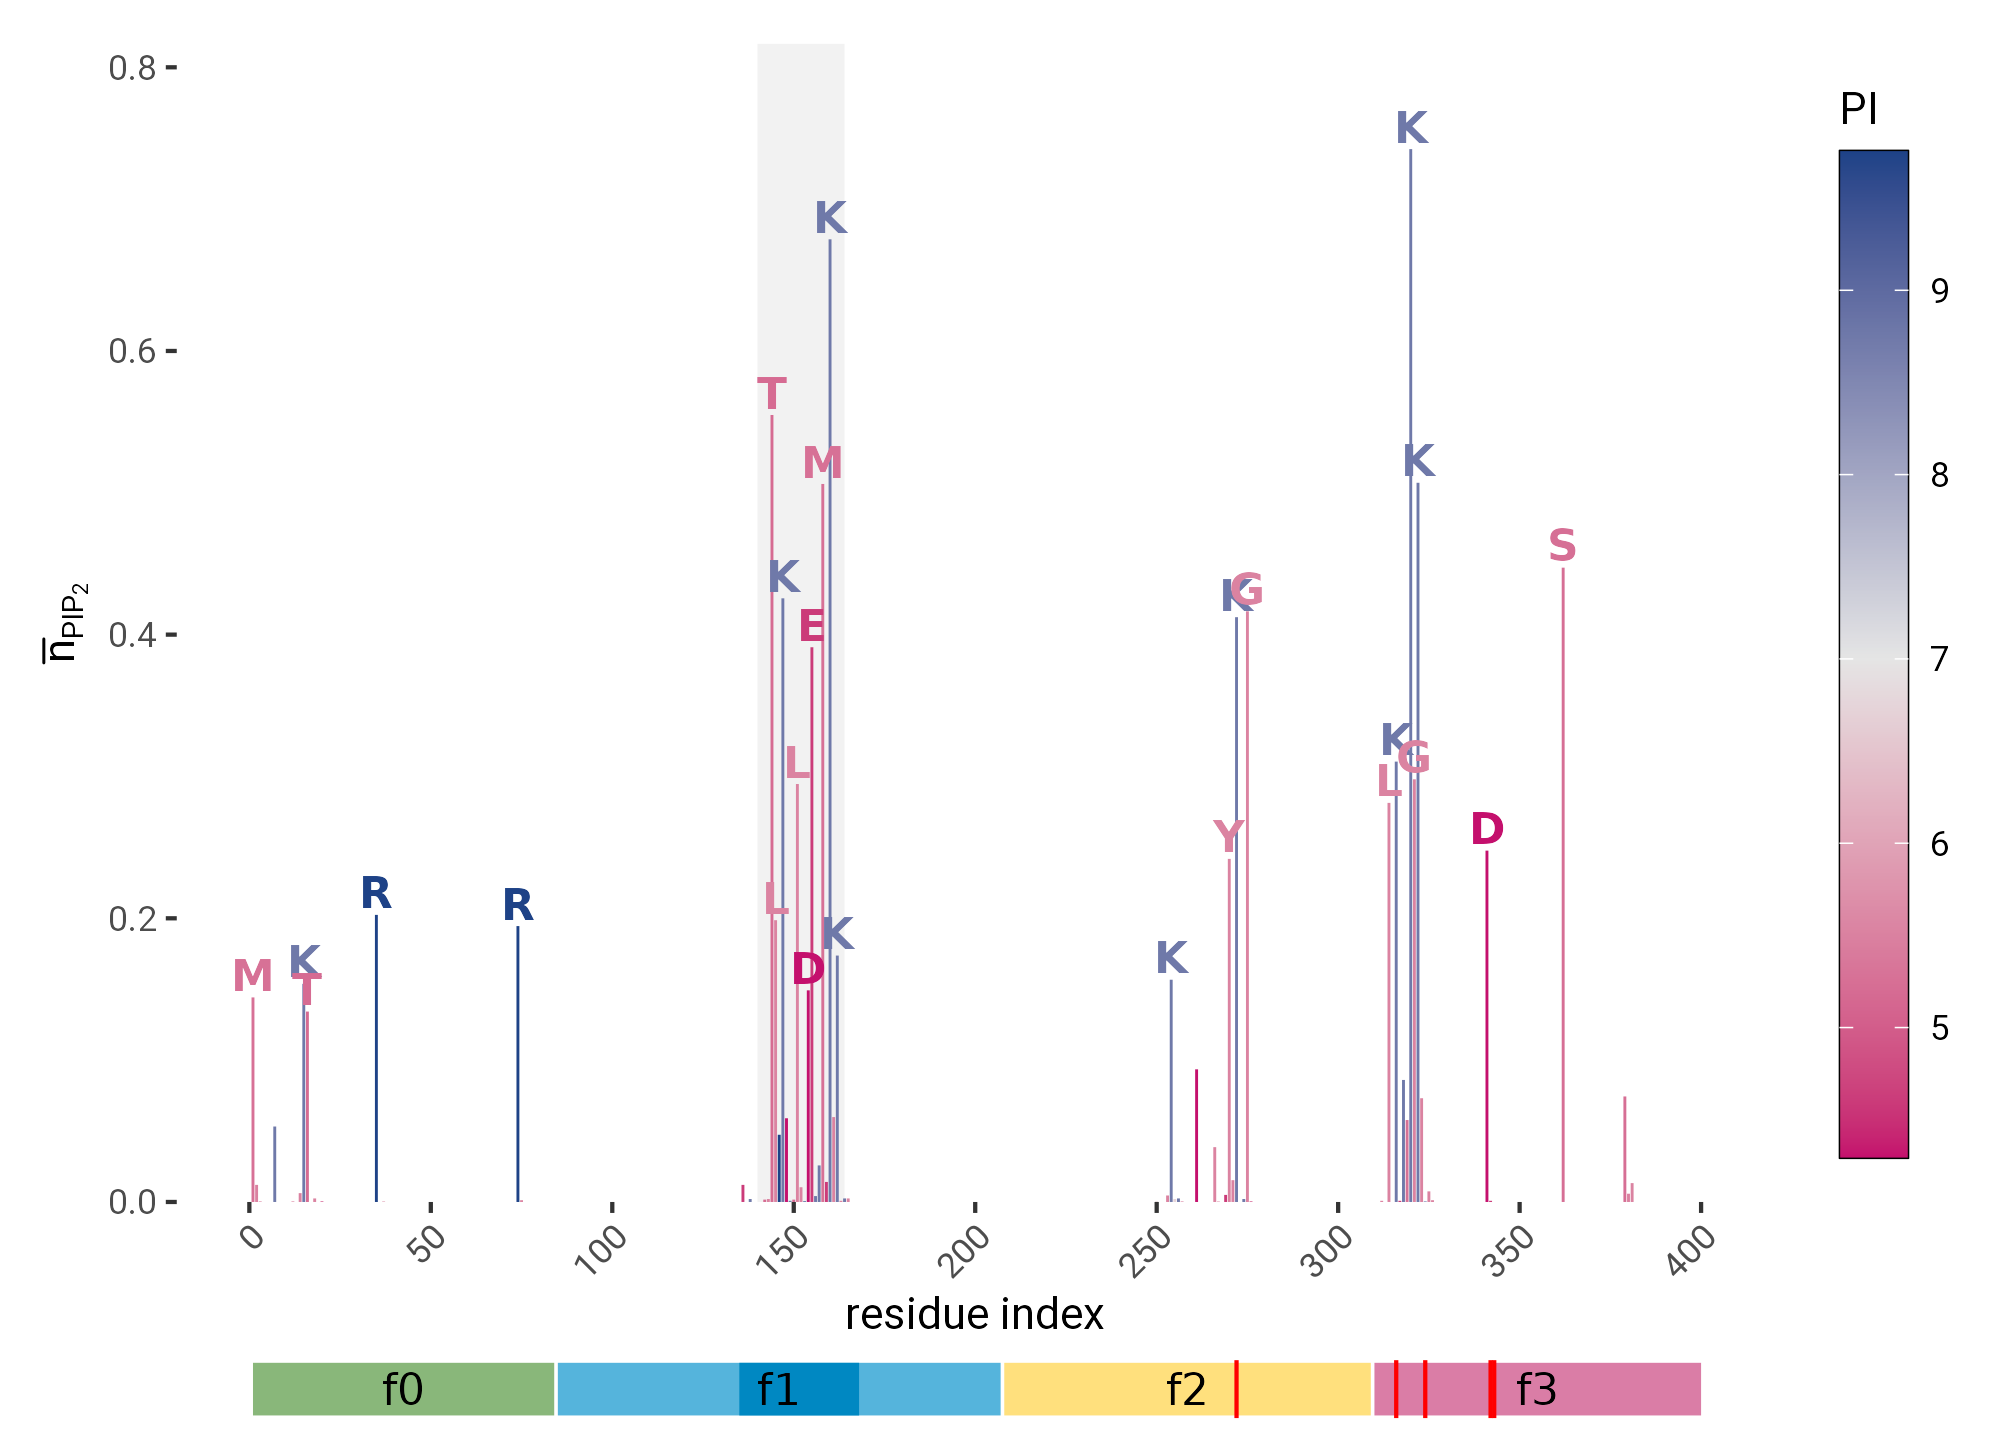
\includegraphics{./results/plots/ferm-ri-npip-1.png}

}

}

\subcaption{\label{fig-ferm-ri-npip}~}
\end{minipage}%
\newline
\begin{minipage}[t]{\linewidth}

{\centering 

\raisebox{-\height}{

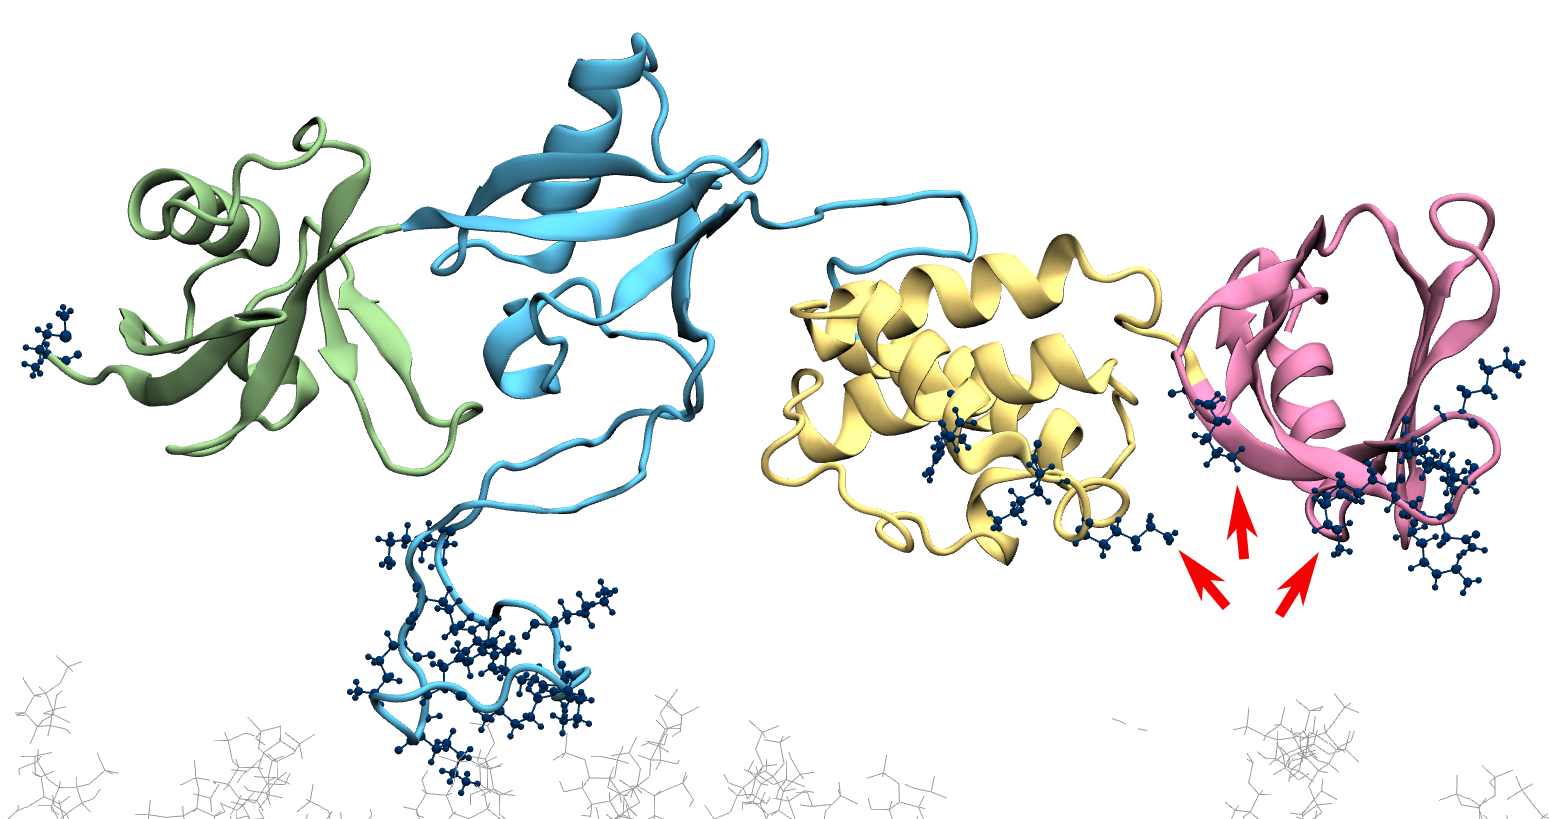
\includegraphics{./assets/vmd/ferm/ferm-residues-transparent-arrows.png}

}

}

\subcaption{\label{fig-ferm-memb-system}~}
\end{minipage}%

\caption{\label{fig-ferm-further}Simulation of the full-length FERM
domain over a 10\% PIP\textsubscript{2}-membrane. \textbf{a)} The Mean
interaction scores of the individual residues across 6 simulations.
Color represents the isoelectric point of the amino acid in isolation
(blue = basic, magenta = acidic). The known PIP\textsubscript{2}
interaction sites K272 of F2 and K316, K324, E342, and K343 of F3 (20)
are highlighted with red lines on the x-axis colorbar and can also be
seen in the cartoon representation in \textbf{b)} where the main
interacting residues are displayed as dark blue stick models.}

\end{figure}

\hypertarget{discussion-and-outlook}{%
\section{Discussion and Outlook}\label{discussion-and-outlook}}

Using MD simulations, we provide mechanistic insight into the membrane
recognition dynamics of Talin. This adds a new mode of interaction that
helps to explain how Talin can find the membrane even when its main
PIP\textsubscript{2} (and integrin) binding sites in F2 and F3 (20) (see
figure Figure~\ref{fig-ferm-memb-system} ) are blocked by autoinhibition
(23). This interaction mode is not characterized by strong binding sites
interacting with one molecule of PIP\textsubscript{2} each, as would be
the conclusion from crystallographic data alone. Rather the cumulative
diffuse interaction of multiple PIP\textsubscript{2} with multiple
residues is what keeps the protein anchored to the membrane. This is
particularly evident in the interaction with the flexible F1 loop, but
also in the F0 domain. While crystal structures of proteins in complex
with PIP\textsubscript{2} typically show a one-to-one ratio of lipid per
binding site (20, 47, 48), possibly due to the nature of the
experimental method, our simulations suggest multiple
PIP\textsubscript{2} molecules binding simultaneously. Similar results
have been observed for Pleckstrin Homology (PH) domain proteins by
Naughton et al. (49). According to their study, this simultaneous
binding of multiple PIP\textsubscript{2} molecules contributes to the
high affinity of the membrane interaction.

Our MD simulations suggest that the F1 loop can find favorable
interactions with PIP\textsubscript{2} across large distances in a large
search volume due to its flexibility. A similar mechanism has also been
shown by Shoemakter et al. (50) and was fittingly coined
``fly-casting''. In the aforementioned publication they focus on the
interaction of unfolded regions with DNA. Our simulations now provide an
example for the concept applied to protein-lipid interactions. It its
well worth noting that, although we mention the greater search space of
the F1 loop as its advantage in recognizing PIP\textsubscript{2}, it has
also been argued that the kinetic advantage of the fly-casting mechanism
comes mainly from the reduction in free energy as the disordered region
folds around the interaction target (51).

The fast binding kinetics are crucial for Talin's function at focal
adhesion sites. As the PIP\textsubscript{2} concentrations increases at
the active focal adhesion site, Talin's FERM F1 loop can perform a quick
recognition. The flexibility of the loop also allows it to anchor the
protein at the membrane even when being stretched under force (up to a
delta of 7 nm, as seen in Figure~\ref{fig-f0f1-vert-pull}). This is akin
to the elastic response seen in focal adhesion kinase (FAK) under force,
in which a 49 AA linker allows for buffering of the force (52). In our
force probe experiments we pulled F0F1 orthogonally off of the membrane.
This was useful in showing the full extension and force resistance of
the loop. \emph{In vivo}, however, Talin's FERM domain is subjected to
forces acting at a 30° angle. This might imply an additional function
for the FERM domain. As it is dragged along the membrane, the diffuse
interactions of the F1 loop and main interaction sites in F2-F3 with
PIP\textsubscript{2} would increase lateral friction along the membrane
as the PIP\textsubscript{2} concentration increases. This could further
localize Talin at active focal adhesion sites.

We conclusively show that the F1 loop is able to interact with the
membrane even from most unfavorable positions. We propose that Talin
mutants lacking the loop, or specifically the basic residues in said
loop, will show reduced or at least slowed-down focal adhesion
maturation, increased lateral diffusion of Talin under force and faster
focal adhesion disassembly.

But recognition is only the first step. It would indeed be fascinating
to also provide mechanistic ideas for the resolution of the
autoinhibition by all-atom simulations of the FERM domain that also
include an inhibiting rod segment. These larger-scale simulations might
then be able to provide evidence for the push--pull mechanism proposed
by Song et al. (12) or result in novel ideas. More generally, we propose
positively charged, intrincsically disordered regions in
PIP\textsubscript{2}-binding domains to promote recognition and help to
maintain the interaction under force, in FERM domains and elsewhere.

\hypertarget{author-contributions}{%
\section{Author Contributions}\label{author-contributions}}

Conceived and designed the experiments:~JB FF FG. Performed the
experiments:~JB FF. Analyzed the data:~JB FF. Contributed
reagents/materials/analysis tools:~FF. Wrote the paper:~JB.

\hypertarget{acknowledgments}{%
\section{Acknowledgments}\label{acknowledgments}}

This project has received funding from the European Research Council
(ERC) under the European Union's Horizon 2020 research and innovation
programme (grant agreement No.~101002812).

This work was supported by the Klaus Tschira Foundation.

\hypertarget{references}{%
\section{References}\label{references}}

\hypertarget{refs}{}
\begin{CSLReferences}{0}{0}
\leavevmode\vadjust pre{\hypertarget{ref-vogelLocalForceGeometry2006}{}}%
\CSLLeftMargin{1. }%
\CSLRightInline{Vogel, V., and M. Sheetz. 2006.
\href{https://doi.org/10.1038/nrm1890}{Local force and geometry sensing
regulate cell functions}. \emph{Nature Reviews Molecular Cell Biology}.
7:265--275.}

\leavevmode\vadjust pre{\hypertarget{ref-oakesStressingLimitsFocal2014}{}}%
\CSLLeftMargin{2. }%
\CSLRightInline{Oakes, P.W., and M.L. Gardel. 2014.
\href{https://doi.org/10.1016/j.ceb.2014.06.003}{Stressing the limits of
focal adhesion mechanosensitivity}. \emph{Current Opinion in Cell
Biology}. 30:68--73.}

\leavevmode\vadjust pre{\hypertarget{ref-schillerMechanosensitivityCompositionalDynamics2013}{}}%
\CSLLeftMargin{3. }%
\CSLRightInline{Schiller, H.B., and R. Fässler. 2013.
\href{https://doi.org/10.1038/embor.2013.49}{Mechanosensitivity and
compositional dynamics of cell\textendash matrix adhesions}. \emph{EMBO
reports}. 14:509--519.}

\leavevmode\vadjust pre{\hypertarget{ref-miroshnikovaAdhesionForcesCortical2018}{}}%
\CSLLeftMargin{4. }%
\CSLRightInline{Miroshnikova, Y.A., H.Q. Le, D. Schneider, T. Thalheim,
M. Rübsam, N. Bremicker, J. Polleux, N. Kamprad, M. Tarantola, I. Wang,
M. Balland, C.M. Niessen, J. Galle, and S.A. Wickström. 2018.
\href{https://doi.org/10.1038/s41556-017-0005-z}{Adhesion forces and
cortical tension couple cell proliferation and differentiation to drive
epidermal stratification}. \emph{Nature Cell Biology}. 20:69--80.}

\leavevmode\vadjust pre{\hypertarget{ref-thamilselvanPressureActivatesColon2004}{}}%
\CSLLeftMargin{5. }%
\CSLRightInline{Thamilselvan, V., and M.D. Basson. 2004.
\href{https://doi.org/10.1053/j.gastro.2003.10.078}{Pressure activates
colon cancer cell adhesion by inside-out focal adhesion complex and
actin cytoskeletal signaling}. \emph{Gastroenterology}. 126:8--18.}

\leavevmode\vadjust pre{\hypertarget{ref-pelletierActivationStateIntegrin1995}{}}%
\CSLLeftMargin{6. }%
\CSLRightInline{Pelletier, A.J., T. Kunicki, Z.M. Ruggeri, and V.
Quaranta. 1995. \href{https://doi.org/10.1074/jbc.270.30.18133}{The
{Activation State} of the {Integrin \(\alpha\)IIb\(\beta\)3 Affects
Outside-in Signals Leading} to {Cell Spreading} and {Focal Adhesion
Kinase Phosphorylation} *}. \emph{Journal of Biological Chemistry}.
270:18133--18140.}

\leavevmode\vadjust pre{\hypertarget{ref-yaoMechanicalResponseTalin2016}{}}%
\CSLLeftMargin{7. }%
\CSLRightInline{Yao, M., B.T. Goult, B. Klapholz, X. Hu, C.P. Toseland,
Y. Guo, P. Cong, M.P. Sheetz, and J. Yan. 2016.
\href{https://doi.org/10.1038/ncomms11966}{The mechanical response of
talin}. \emph{Nature Communications}. 7:11966.}

\leavevmode\vadjust pre{\hypertarget{ref-tadokoroTalinBindingIntegrin2003}{}}%
\CSLLeftMargin{8. }%
\CSLRightInline{Tadokoro, S., S.J. Shattil, K. Eto, V. Tai, R.C.
Liddington, J.M. de Pereda, M.H. Ginsberg, and D.A. Calderwood. 2003.
\href{https://doi.org/10.1126/science.1086652}{Talin {Binding} to
{Integrin} ß {Tails}: {A Final Common Step} in {Integrin Activation}}.
\emph{Science}. 302:103--106.}

\leavevmode\vadjust pre{\hypertarget{ref-chishtiFERMDomainUnique1998}{}}%
\CSLLeftMargin{9. }%
\CSLRightInline{Chishti, A.H., A.C. Kim, S.M. Marfatia, M. Lutchman, M.
Hanspal, H. Jindal, S.-C. Liu, P.S. Low, G.A. Rouleau, N. Mohandas, J.A.
Chasis, J.G. Conboy, P. Gascard, Y. Takakuwa, S.-C. Huang, E.J.B. Jr, A.
Bretscher, R.G. Fehon, J.F. Gusella, V. Ramesh, F. Solomon, V.T.
Marchesi, S. Tsukita, S. Tsukita, M. Arpin, D. Louvard, N.K. Tonks, J.M.
Anderson, A.S. Fanning, P.J. Bryant, D.F. Woods, and K.B. Hoover. 1998.
\href{https://doi.org/10.1016/S0968-0004(98)01237-7}{The {FERM} domain:
A unique module involved in the linkage of cytoplasmic proteins to the
membrane}. \emph{Trends in Biochemical Sciences}. 23:281--282.}

\leavevmode\vadjust pre{\hypertarget{ref-maniFERMDomainPhosphoinositide2011}{}}%
\CSLLeftMargin{10. }%
\CSLRightInline{Mani, T., R.F. Hennigan, L.A. Foster, D.G. Conrady, A.B.
Herr, and W. Ip. 2011. \href{https://doi.org/10.1128/MCB.00609-10}{{FERM
Domain Phosphoinositide Binding Targets Merlin} to the {Membrane} and
{Is Essential} for {Its Growth-Suppressive Function}}. \emph{Molecular
and Cellular Biology}. 31:1983--1996.}

\leavevmode\vadjust pre{\hypertarget{ref-dasMolecularMechanotransductionPathway2015}{}}%
\CSLLeftMargin{11. }%
\CSLRightInline{Das, T., K. Safferling, S. Rausch, N. Grabe, H. Boehm,
and J.P. Spatz. 2015. \href{https://doi.org/10.1038/ncb3115}{A molecular
mechanotransduction pathway regulates collective migration of epithelial
cells}. \emph{Nature Cell Biology}. 17:276--287.}

\leavevmode\vadjust pre{\hypertarget{ref-songNovelMembranedependentSwitch2012a}{}}%
\CSLLeftMargin{12. }%
\CSLRightInline{Song, X., J. Yang, J. Hirbawi, S. Ye, H.D. Perera, E.
Goksoy, P. Dwivedi, E.F. Plow, R. Zhang, and J. Qin. 2012.
\href{https://doi.org/10.1038/cr.2012.97}{A novel membrane-dependent
on/off switch mechanism of talin {FERM} domain at sites of cell
adhesion}. \emph{Cell Research}. 22:1533--1545.}

\leavevmode\vadjust pre{\hypertarget{ref-goultStructureDoubleUbiquitinlike2010}{}}%
\CSLLeftMargin{13. }%
\CSLRightInline{Goult, B.T., M. Bouaouina, P.R. Elliott, N. Bate, B.
Patel, A.R. Gingras, J.G. Grossmann, G.C.K. Roberts, D.A. Calderwood,
D.R. Critchley, and I.L. Barsukov. 2010.
\href{https://doi.org/10.1038/emboj.2010.4}{Structure of a double
ubiquitin-like domain in the talin head: A role in integrin activation}.
\emph{The EMBO Journal}. 29:1069--1080.}

\leavevmode\vadjust pre{\hypertarget{ref-elliottStructureTalinHead2010}{}}%
\CSLLeftMargin{14. }%
\CSLRightInline{Elliott, P.R., B.T. Goult, P.M. Kopp, N. Bate, J.G.
Grossmann, G.C.K. Roberts, D.R. Critchley, and I.L. Barsukov. 2010.
\href{https://doi.org/10.1016/j.str.2010.07.011}{The {Structure} of the
{Talin Head Reveals} a {Novel~Extended Conformation} of the {FERM
Domain}}. \emph{Structure(London, England:1993)}. 18:1289--1299.}

\leavevmode\vadjust pre{\hypertarget{ref-calderwoodTalinHeadDomain1999}{}}%
\CSLLeftMargin{15. }%
\CSLRightInline{Calderwood, D.A., R. Zent, R. Grant, D.J.G. Rees, R.O.
Hynes, and M.H. Ginsberg. 1999.
\href{https://doi.org/10.1074/jbc.274.40.28071}{The {Talin Head Domain
Binds} to {Integrin} {\(\beta\)} {Subunit Cytoplasmic Tails} and
{Regulates Integrin Activation} *}. \emph{Journal of Biological
Chemistry}. 274:28071--28074.}

\leavevmode\vadjust pre{\hypertarget{ref-calderwoodTalinsKindlinsPartners2013}{}}%
\CSLLeftMargin{16. }%
\CSLRightInline{Calderwood, D.A., I.D. Campbell, and D.R. Critchley.
2013. \href{https://doi.org/10.1038/nrm3624}{Talins and kindlins:
Partners in integrin-mediated adhesion}. \emph{Nature Reviews Molecular
Cell Biology}. 14:503--517.}

\leavevmode\vadjust pre{\hypertarget{ref-horwitzInteractionPlasmaMembrane1986}{}}%
\CSLLeftMargin{17. }%
\CSLRightInline{Horwitz, A., K. Duggan, C. Buck, M.C. Beckerle, and K.
Burridge. 1986. \href{https://doi.org/10.1038/320531a0}{Interaction of
plasma membrane fibronectin receptor with talin\textemdash a
transmembrane linkage}. \emph{Nature}. 320:531--533.}

\leavevmode\vadjust pre{\hypertarget{ref-mccannLWEQModuleConserved1997}{}}%
\CSLLeftMargin{18. }%
\CSLRightInline{McCann, R.O., and S.W. Craig. 1997.
\href{https://doi.org/10.1073/pnas.94.11.5679}{The {I}/{LWEQ} module: A
conserved sequence that signifies {F-actin} binding in functionally
diverse proteins from yeast to mammals}. \emph{Proceedings of the
National Academy of Sciences}. 94:5679--5684.}

\leavevmode\vadjust pre{\hypertarget{ref-klapholzTalinMasterIntegrin2017}{}}%
\CSLLeftMargin{19. }%
\CSLRightInline{Klapholz, B., and N.H. Brown. 2017.
\href{https://doi.org/10.1242/jcs.190991}{Talin \textendash{} the master
of integrin adhesions}. \emph{Journal of Cell Science}. 130:2435--2446.}

\leavevmode\vadjust pre{\hypertarget{ref-chinthalapudiInteractionTalinCell2018a}{}}%
\CSLLeftMargin{20. }%
\CSLRightInline{Chinthalapudi, K., E.S. Rangarajan, and T. Izard. 2018.
\href{https://doi.org/10.1073/pnas.1806275115}{The interaction of talin
with the cell membrane is essential for integrin activation and focal
adhesion formation}. \emph{Proceedings of the National Academy of
Sciences of the United States of America}. 115:10339--10344.}

\leavevmode\vadjust pre{\hypertarget{ref-saltelNewPIP22009}{}}%
\CSLLeftMargin{21. }%
\CSLRightInline{Saltel, F., E. Mortier, V.P. Hytönen, M.-C. Jacquier, P.
Zimmermann, V. Vogel, W. Liu, and B. Wehrle-Haller. 2009.
\href{https://doi.org/10.1083/jcb.200908134}{New {PI}(4,5){P2-} and
membrane proximal integrin\textendash binding motifs in the talin head
control {\(B\)}3-integrin clustering}. \emph{Journal of Cell Biology}.
187:715--731.}

\leavevmode\vadjust pre{\hypertarget{ref-bannoSubcellularLocalizationTalin2012}{}}%
\CSLLeftMargin{22. }%
\CSLRightInline{Banno, A., B.T. Goult, H. Lee, N. Bate, D.R. Critchley,
and M.H. Ginsberg. 2012.
\href{https://doi.org/10.1074/jbc.M112.341214}{Subcellular
{Localization} of {Talin Is Regulated} by {Inter-domain Interactions}
*}. \emph{Journal of Biological Chemistry}. 287:13799--13812.}

\leavevmode\vadjust pre{\hypertarget{ref-deddenArchitectureTalin1Reveals2019a}{}}%
\CSLLeftMargin{23. }%
\CSLRightInline{Dedden, D., S. Schumacher, C.F. Kelley, M. Zacharias, C.
Biertümpfel, R. Fässler, and N. Mizuno. 2019.
\href{https://doi.org/10.1016/j.cell.2019.08.034}{The {Architecture} of
{Talin1 Reveals} an {Autoinhibition Mechanism}}. \emph{Cell}.
179:120--131.e13.}

\leavevmode\vadjust pre{\hypertarget{ref-buyanMultiscaleSimulationsSuggest2016}{}}%
\CSLLeftMargin{24. }%
\CSLRightInline{Buyan, A., A.C. Kalli, and M.S.P. Sansom. 2016.
\href{https://doi.org/10.1371/journal.pcbi.1005028}{Multiscale
{Simulations Suggest} a {Mechanism} for the {Association} of the {Dok7
PH Domain} with {PIP-Containing Membranes}}. \emph{PLOS Computational
Biology}. 12:e1005028.}

\leavevmode\vadjust pre{\hypertarget{ref-zhouMechanismFocalAdhesion2015}{}}%
\CSLLeftMargin{25. }%
\CSLRightInline{Zhou, J., C. Aponte-Santamaría, S. Sturm, J.T.
Bullerjahn, A. Bronowska, and F. Gräter. 2015.
\href{https://doi.org/10.1371/journal.pcbi.1004593}{Mechanism of {Focal
Adhesion Kinase Mechanosensing}}. \emph{PLOS Computational Biology}.
11:e1004593.}

\leavevmode\vadjust pre{\hypertarget{ref-berendsenGROMACSMessagepassingParallel1995}{}}%
\CSLLeftMargin{26. }%
\CSLRightInline{Berendsen, H.J.C., D. van der Spoel, and R. van Drunen.
1995. \href{https://doi.org/10.1016/0010-4655(95)00042-E}{{GROMACS}: {A}
message-passing parallel molecular dynamics implementation}.
\emph{Computer Physics Communications}. 91:43--56.}

\leavevmode\vadjust pre{\hypertarget{ref-abrahamGROMACSHighPerformance2015}{}}%
\CSLLeftMargin{27. }%
\CSLRightInline{Abraham, M.J., T. Murtola, R. Schulz, S. Páll, J.C.
Smith, B. Hess, and E. Lindahl. 2015.
\href{https://doi.org/10.1016/j.softx.2015.06.001}{{GROMACS}: {High}
performance molecular simulations through multi-level parallelism from
laptops to supercomputers}. \emph{SoftwareX}. 1--2:19--25.}

\leavevmode\vadjust pre{\hypertarget{ref-lindahlGROMACS2020Source2020}{}}%
\CSLLeftMargin{28. }%
\CSLRightInline{Lindahl, Abraham, Hess, and van der Spoel. 2020-01-01,
2020-01. \href{https://doi.org/10.5281/zenodo.3562495}{{GROMACS} 2020
source code}. {Zenodo}.}

\leavevmode\vadjust pre{\hypertarget{ref-marti-renomComparativeProteinStructure2000}{}}%
\CSLLeftMargin{29. }%
\CSLRightInline{Martí-Renom, M.A., A.C. Stuart, A. Fiser, R. Sánchez, F.
Melo, and A. Sali. 2000.
\href{https://doi.org/10.1146/annurev.biophys.29.1.291}{Comparative
protein structure modeling of genes and genomes}. \emph{Annual Review of
Biophysics and Biomolecular Structure}. 29:291--325.}

\leavevmode\vadjust pre{\hypertarget{ref-webbComparativeProteinStructure2016}{}}%
\CSLLeftMargin{30. }%
\CSLRightInline{Webb, B., and A. Sali. 2016.
\href{https://doi.org/10.1002/cpps.20}{Comparative {Protein Structure
Modeling Using MODELLER}}. \emph{Current Protocols in Protein Science}.
86:2.9.1--2.9.37.}

\leavevmode\vadjust pre{\hypertarget{ref-pettersenUCSFChimeraVisualization2004}{}}%
\CSLLeftMargin{31. }%
\CSLRightInline{Pettersen, E.F., T.D. Goddard, C.C. Huang, G.S. Couch,
D.M. Greenblatt, E.C. Meng, and T.E. Ferrin. 2004.
\href{https://doi.org/10.1002/jcc.20084}{{UCSF Chimera--a} visualization
system for exploratory research and analysis}. \emph{Journal of
Computational Chemistry}. 25:1605--1612.}

\leavevmode\vadjust pre{\hypertarget{ref-brooksCHARMMBiomolecularSimulation2009}{}}%
\CSLLeftMargin{32. }%
\CSLRightInline{Brooks, B.R., C.L. Brooks, A.D. Mackerell, L. Nilsson,
R.J. Petrella, B. Roux, Y. Won, G. Archontis, C. Bartels, S. Boresch, A.
Caflisch, L. Caves, Q. Cui, A.R. Dinner, M. Feig, S. Fischer, J. Gao, M.
Hodoscek, W. Im, K. Kuczera, T. Lazaridis, J. Ma, V. Ovchinnikov, E.
Paci, R.W. Pastor, C.B. Post, J.Z. Pu, M. Schaefer, B. Tidor, R.M.
Venable, H.L. Woodcock, X. Wu, W. Yang, D.M. York, and M. Karplus. 2009.
\href{https://doi.org/10.1002/jcc.21287}{{CHARMM}: {The} biomolecular
simulation program}. \emph{Journal of Computational Chemistry}.
30:1545--1614.}

\leavevmode\vadjust pre{\hypertarget{ref-joCHARMMGUIWebbasedGraphical2008}{}}%
\CSLLeftMargin{33. }%
\CSLRightInline{Jo, S., T. Kim, V.G. Iyer, and W. Im. 2008.
\href{https://doi.org/10.1002/jcc.20945}{{CHARMM-GUI}: A web-based
graphical user interface for {CHARMM}}. \emph{Journal of Computational
Chemistry}. 29:1859--1865.}

\leavevmode\vadjust pre{\hypertarget{ref-leeCHARMMGUIInputGenerator2016}{}}%
\CSLLeftMargin{34. }%
\CSLRightInline{Lee, J., X. Cheng, J.M. Swails, M.S. Yeom, P.K. Eastman,
J.A. Lemkul, S. Wei, J. Buckner, J.C. Jeong, Y. Qi, S. Jo, V.S. Pande,
D.A. Case, C.L. Brooks, A.D. MacKerell, J.B. Klauda, and W. Im. 2016.
\href{https://doi.org/10.1021/acs.jctc.5b00935}{{CHARMM-GUI Input
Generator} for {NAMD}, {GROMACS}, {AMBER}, {OpenMM}, and
{CHARMM}/{OpenMM Simulations Using} the {CHARMM36 Additive Force
Field}}. \emph{Journal of Chemical Theory and Computation}.
12:405--413.}

\leavevmode\vadjust pre{\hypertarget{ref-hooverCanonicalDynamicsEquilibrium1985}{}}%
\CSLLeftMargin{35. }%
\CSLRightInline{Hoover, W.G. 1985.
\href{https://doi.org/10.1103/PhysRevA.31.1695}{Canonical dynamics:
{Equilibrium} phase-space distributions}. \emph{Physical Review A}.
31:1695--1697.}

\leavevmode\vadjust pre{\hypertarget{ref-noseUnifiedFormulationConstant1984}{}}%
\CSLLeftMargin{36. }%
\CSLRightInline{Nosé, S. 1984. \href{https://doi.org/10.1063/1.447334}{A
unified formulation of the constant temperature molecular dynamics
methods}. \emph{The Journal of Chemical Physics}. 81:511--519.}

\leavevmode\vadjust pre{\hypertarget{ref-parrinelloPolymorphicTransitionsSingle1981}{}}%
\CSLLeftMargin{37. }%
\CSLRightInline{Parrinello, M., and A. Rahman. 1981.
\href{https://doi.org/10.1063/1.328693}{Polymorphic transitions in
single crystals: {A} new molecular dynamics method}. \emph{Journal of
Applied Physics}. 52:7182--7190.}

\leavevmode\vadjust pre{\hypertarget{ref-mercadanteCONANToolDecode2018}{}}%
\CSLLeftMargin{38. }%
\CSLRightInline{Mercadante, D., F. Gräter, and C. Daday. 2018.
\href{https://doi.org/10.1016/j.bpj.2018.01.033}{{CONAN}: {A Tool} to
{Decode Dynamical Information} from {Molecular Interaction Maps}}.
\emph{Biophysical Journal}. 114:1267--1273.}

\leavevmode\vadjust pre{\hypertarget{ref-landauTargetsPackageDynamic2021}{}}%
\CSLLeftMargin{39. }%
\CSLRightInline{Landau, W.M. 2021. The targets {R} package: A dynamic
{Make-like} function-oriented pipeline toolkit for reproducibility and
high-performance computing. \emph{Journal of Open Source Software}.
6:2959.}

\leavevmode\vadjust pre{\hypertarget{ref-ggplot}{}}%
\CSLLeftMargin{40. }%
\CSLRightInline{Wickham, H. 2016. Ggplot2: {Elegant} graphics for data
analysis. {Springer-Verlag New York}.}

\leavevmode\vadjust pre{\hypertarget{ref-molstar}{}}%
\CSLLeftMargin{41. }%
\CSLRightInline{Sehnal, D., S. Bittrich, M. Deshpande, R. Svobodová, K.
Berka, V. Bazgier, S. Velankar, S.K. Burley, J. Koča, and A.S. Rose.
2021. \href{https://doi.org/10.1093/nar/gkab314}{Mol* {Viewer}: Modern
web app for {3D} visualization and analysis of large biomolecular
structures}. \emph{Nucleic Acids Research}. 49:W431--W437.}

\leavevmode\vadjust pre{\hypertarget{ref-blender}{}}%
\CSLLeftMargin{42. }%
\CSLRightInline{Community, B.O. 2018. Blender - a {3D} modelling and
rendering package.}

\leavevmode\vadjust pre{\hypertarget{ref-vmd}{}}%
\CSLLeftMargin{43. }%
\CSLRightInline{Humphrey, W., A. Dalke, and K. Schulten. 1996. {VMD}
\textendash{} {Visual Molecular Dynamics}. \emph{Journal of Molecular
Graphics}. 14:33--38.}

\leavevmode\vadjust pre{\hypertarget{ref-quarto}{}}%
\CSLLeftMargin{44. }%
\CSLRightInline{Allaire, J.J., C. Teague, C. Scheidegger, Y. Xie, and C.
Dervieux. 2022. \href{https://doi.org/10.5281/zenodo.5960048}{Quarto}.}

\leavevmode\vadjust pre{\hypertarget{ref-knitr}{}}%
\CSLLeftMargin{45. }%
\CSLRightInline{Xie, Y. 2015. Dynamic documents with {R} and knitr.
Second. {Boca Raton, Florida}: {Chapman and Hall/CRC}.}

\leavevmode\vadjust pre{\hypertarget{ref-rbetterposter}{}}%
\CSLLeftMargin{46. }%
\CSLRightInline{Aden-Buie, G. 2022. Betterposter: {A} better scientific
poster.}

\leavevmode\vadjust pre{\hypertarget{ref-chinthalapudiLipidBindingPromotes2018}{}}%
\CSLLeftMargin{47. }%
\CSLRightInline{Chinthalapudi, K., V. Mandati, J. Zheng, A.J. Sharff, G.
Bricogne, P.R. Griffin, J. Kissil, and T. Izard. 2018.
\href{https://doi.org/10.1038/s41467-018-03648-4}{Lipid binding promotes
the open conformation and tumor-suppressive activity of neurofibromin
2}. \emph{Nature Communications}. 9:1338.}

\leavevmode\vadjust pre{\hypertarget{ref-jianMolecularBasisCooperative2015}{}}%
\CSLLeftMargin{48. }%
\CSLRightInline{Jian, X., W.-K. Tang, P. Zhai, N.S. Roy, R. Luo, J.M.
Gruschus, M.E. Yohe, P.-W. Chen, Y. Li, R.A. Byrd, D. Xia, and P.A.
Randazzo. 2015.
\href{https://doi.org/10.1016/j.str.2015.08.008}{Molecular {Basis} for
{Cooperative Binding} of {Anionic Phospholipids} to the {PH Domain} of
the {Arf GAP ASAP1}}. \emph{Structure}. 23:1977--1988.}

\leavevmode\vadjust pre{\hypertarget{ref-naughtonModesInteractionPleckstrin2018}{}}%
\CSLLeftMargin{49. }%
\CSLRightInline{Naughton, F.B., A.C. Kalli, and M.S.P. Sansom. 2018.
\href{https://doi.org/10.1016/j.jmb.2017.12.011}{Modes of {Interaction}
of {Pleckstrin Homology Domains} with {Membranes}: {Toward} a
{Computational Biochemistry} of {Membrane Recognition}}. \emph{Journal
of Molecular Biology}. 430:372--388.}

\leavevmode\vadjust pre{\hypertarget{ref-shoemakerSpeedingMolecularRecognition2000}{}}%
\CSLLeftMargin{50. }%
\CSLRightInline{Shoemaker, B.A., J.J. Portman, and P.G. Wolynes. 2000.
\href{https://doi.org/10.1073/pnas.160259697}{Speeding molecular
recognition by using the folding funnel: The fly-casting mechanism}.
\emph{Proceedings of the National Academy of Sciences of the United
States of America}. 97:8868--8873.}

\leavevmode\vadjust pre{\hypertarget{ref-huangKineticAdvantageIntrinsically2009}{}}%
\CSLLeftMargin{51. }%
\CSLRightInline{Huang, Y., and Z. Liu. 2009.
\href{https://doi.org/10.1016/j.jmb.2009.09.010}{Kinetic {Advantage} of
{Intrinsically Disordered Proteins} in {Coupled
Folding}\textendash{{Binding Process}}: {A Critical Assessment} of the
{``{Fly-Casting}''} {Mechanism}}. \emph{Journal of Molecular Biology}.
393:1143--1159.}

\leavevmode\vadjust pre{\hypertarget{ref-bauerStructuralMechanisticInsights2019}{}}%
\CSLLeftMargin{52. }%
\CSLRightInline{Bauer, M.S., F. Baumann, C. Daday, P. Redondo, E.
Durner, M.A. Jobst, L.F. Milles, D. Mercadante, D.A. Pippig, H.E. Gaub,
F. Gräter, and D. Lietha. 2019.
\href{https://doi.org/10.1073/pnas.1820567116}{Structural and
mechanistic insights into mechanoactivation of focal adhesion kinase}.
\emph{Proceedings of the National Academy of Sciences}. 116:6766--6774.}

\end{CSLReferences}

\hypertarget{supplementary-material}{%
\section{Supplementary Material}\label{supplementary-material}}

\hypertarget{sec-system}{%
\subsection{Simulation System}\label{sec-system}}

\begin{tcolorbox}[enhanced jigsaw, arc=.35mm, colbacktitle=quarto-callout-note-color!10!white, colback=white, left=2mm, breakable, colframe=quarto-callout-note-color-frame, bottomrule=.15mm, leftrule=.75mm, rightrule=.15mm, title=\textcolor{quarto-callout-note-color}{\faInfo}\hspace{0.5em}{Note}, bottomtitle=1mm, opacitybacktitle=0.6, toprule=.15mm, opacityback=0, coltitle=black, toptitle=1mm, titlerule=0mm]
This interactive display is only available in the web version:
\url{https://hits-mbm-dev.github.io/paper-talin-loop/}
\end{tcolorbox}

\hypertarget{scripts}{%
\subsection{Scripts}\label{scripts}}

\begin{tcolorbox}[enhanced jigsaw, arc=.35mm, colbacktitle=quarto-callout-note-color!10!white, colback=white, left=2mm, breakable, colframe=quarto-callout-note-color-frame, bottomrule=.15mm, leftrule=.75mm, rightrule=.15mm, title=\textcolor{quarto-callout-note-color}{\faInfo}\hspace{0.5em}{Note}, bottomtitle=1mm, opacitybacktitle=0.6, toprule=.15mm, opacityback=0, coltitle=black, toptitle=1mm, titlerule=0mm]
Analysis scripts, setup scripts and production trajectories will be
uploaded and linked here.
\end{tcolorbox}

\hypertarget{supplementary-plots-and-tables}{%
\subsection{Supplementary Plots and
Tables}\label{supplementary-plots-and-tables}}

\begin{figure}

\begin{minipage}[t]{0.50\linewidth}

{\centering 

\raisebox{-\height}{

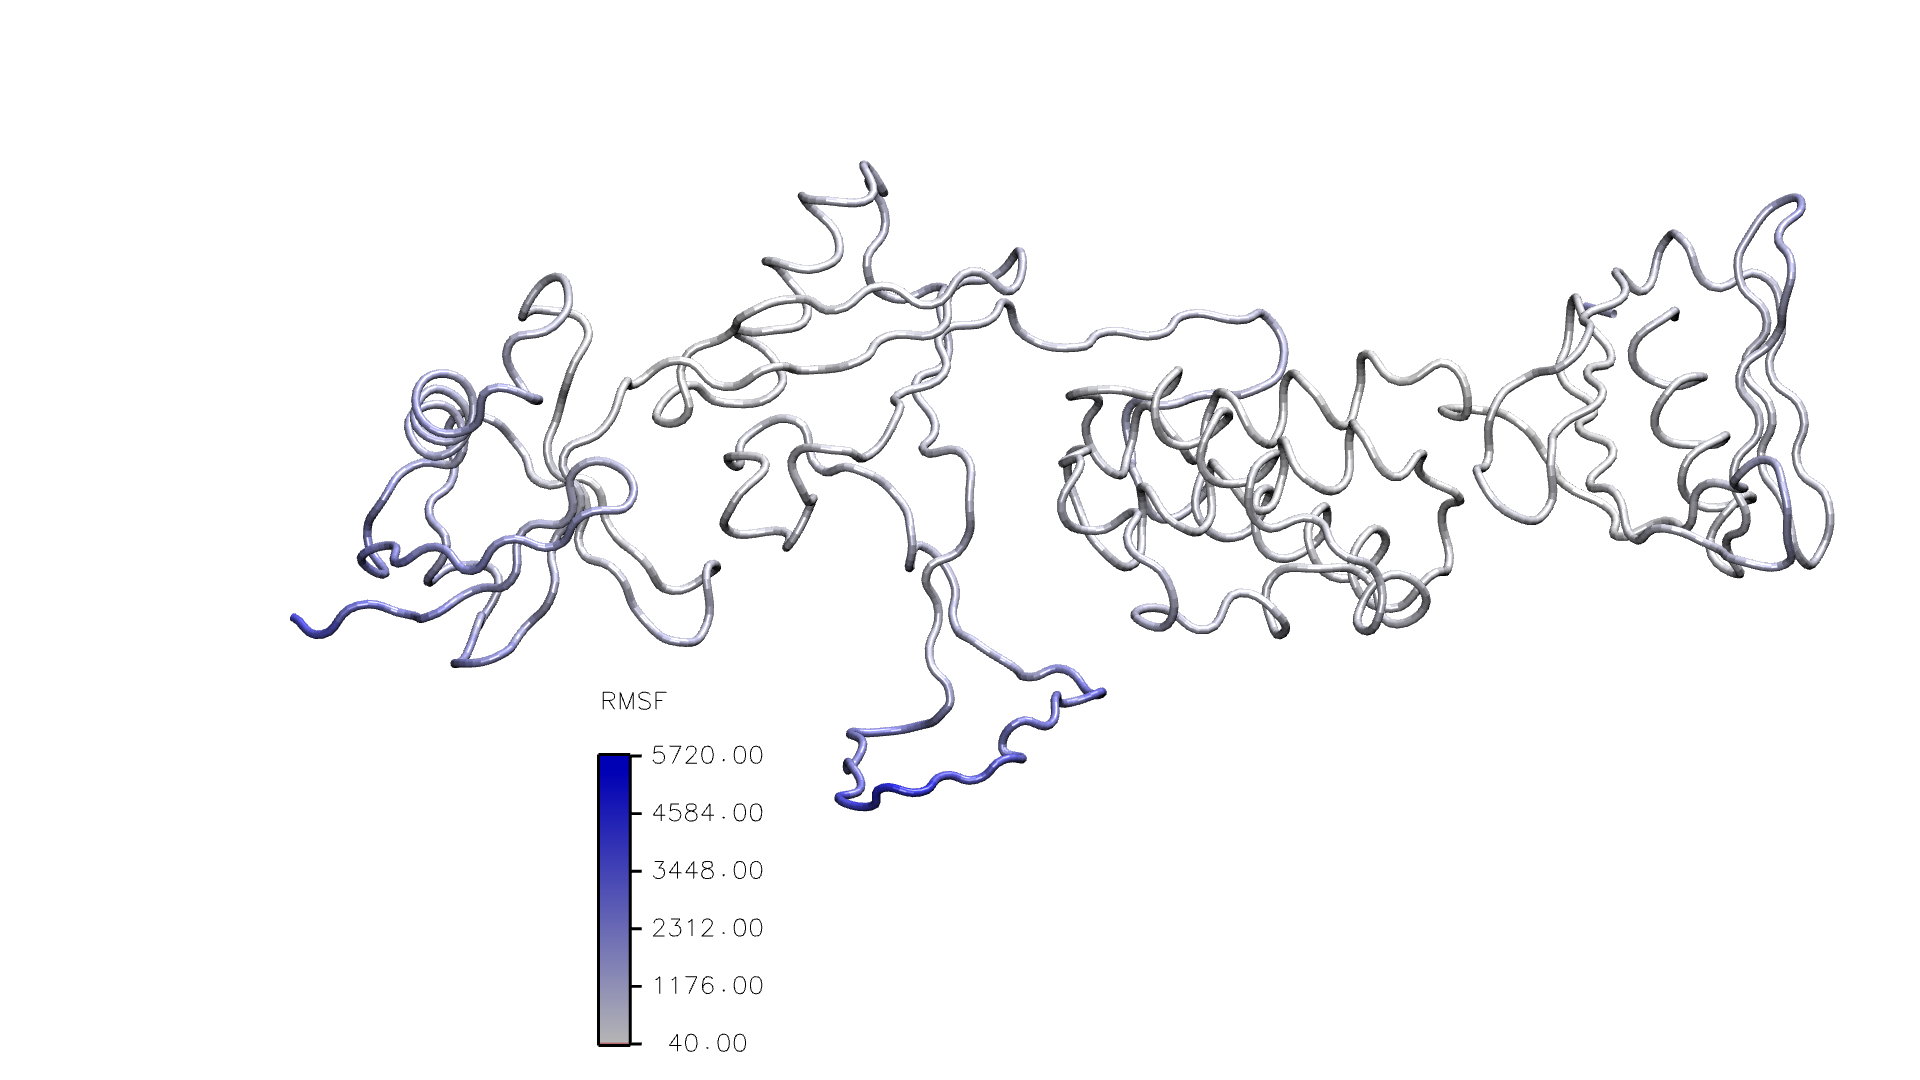
\includegraphics{./assets/results/figures/loop-rmsf.png}

}

}

\subcaption{\label{fig-loop-rmsf}~}
\end{minipage}%
%
\begin{minipage}[t]{0.50\linewidth}

{\centering 

\raisebox{-\height}{

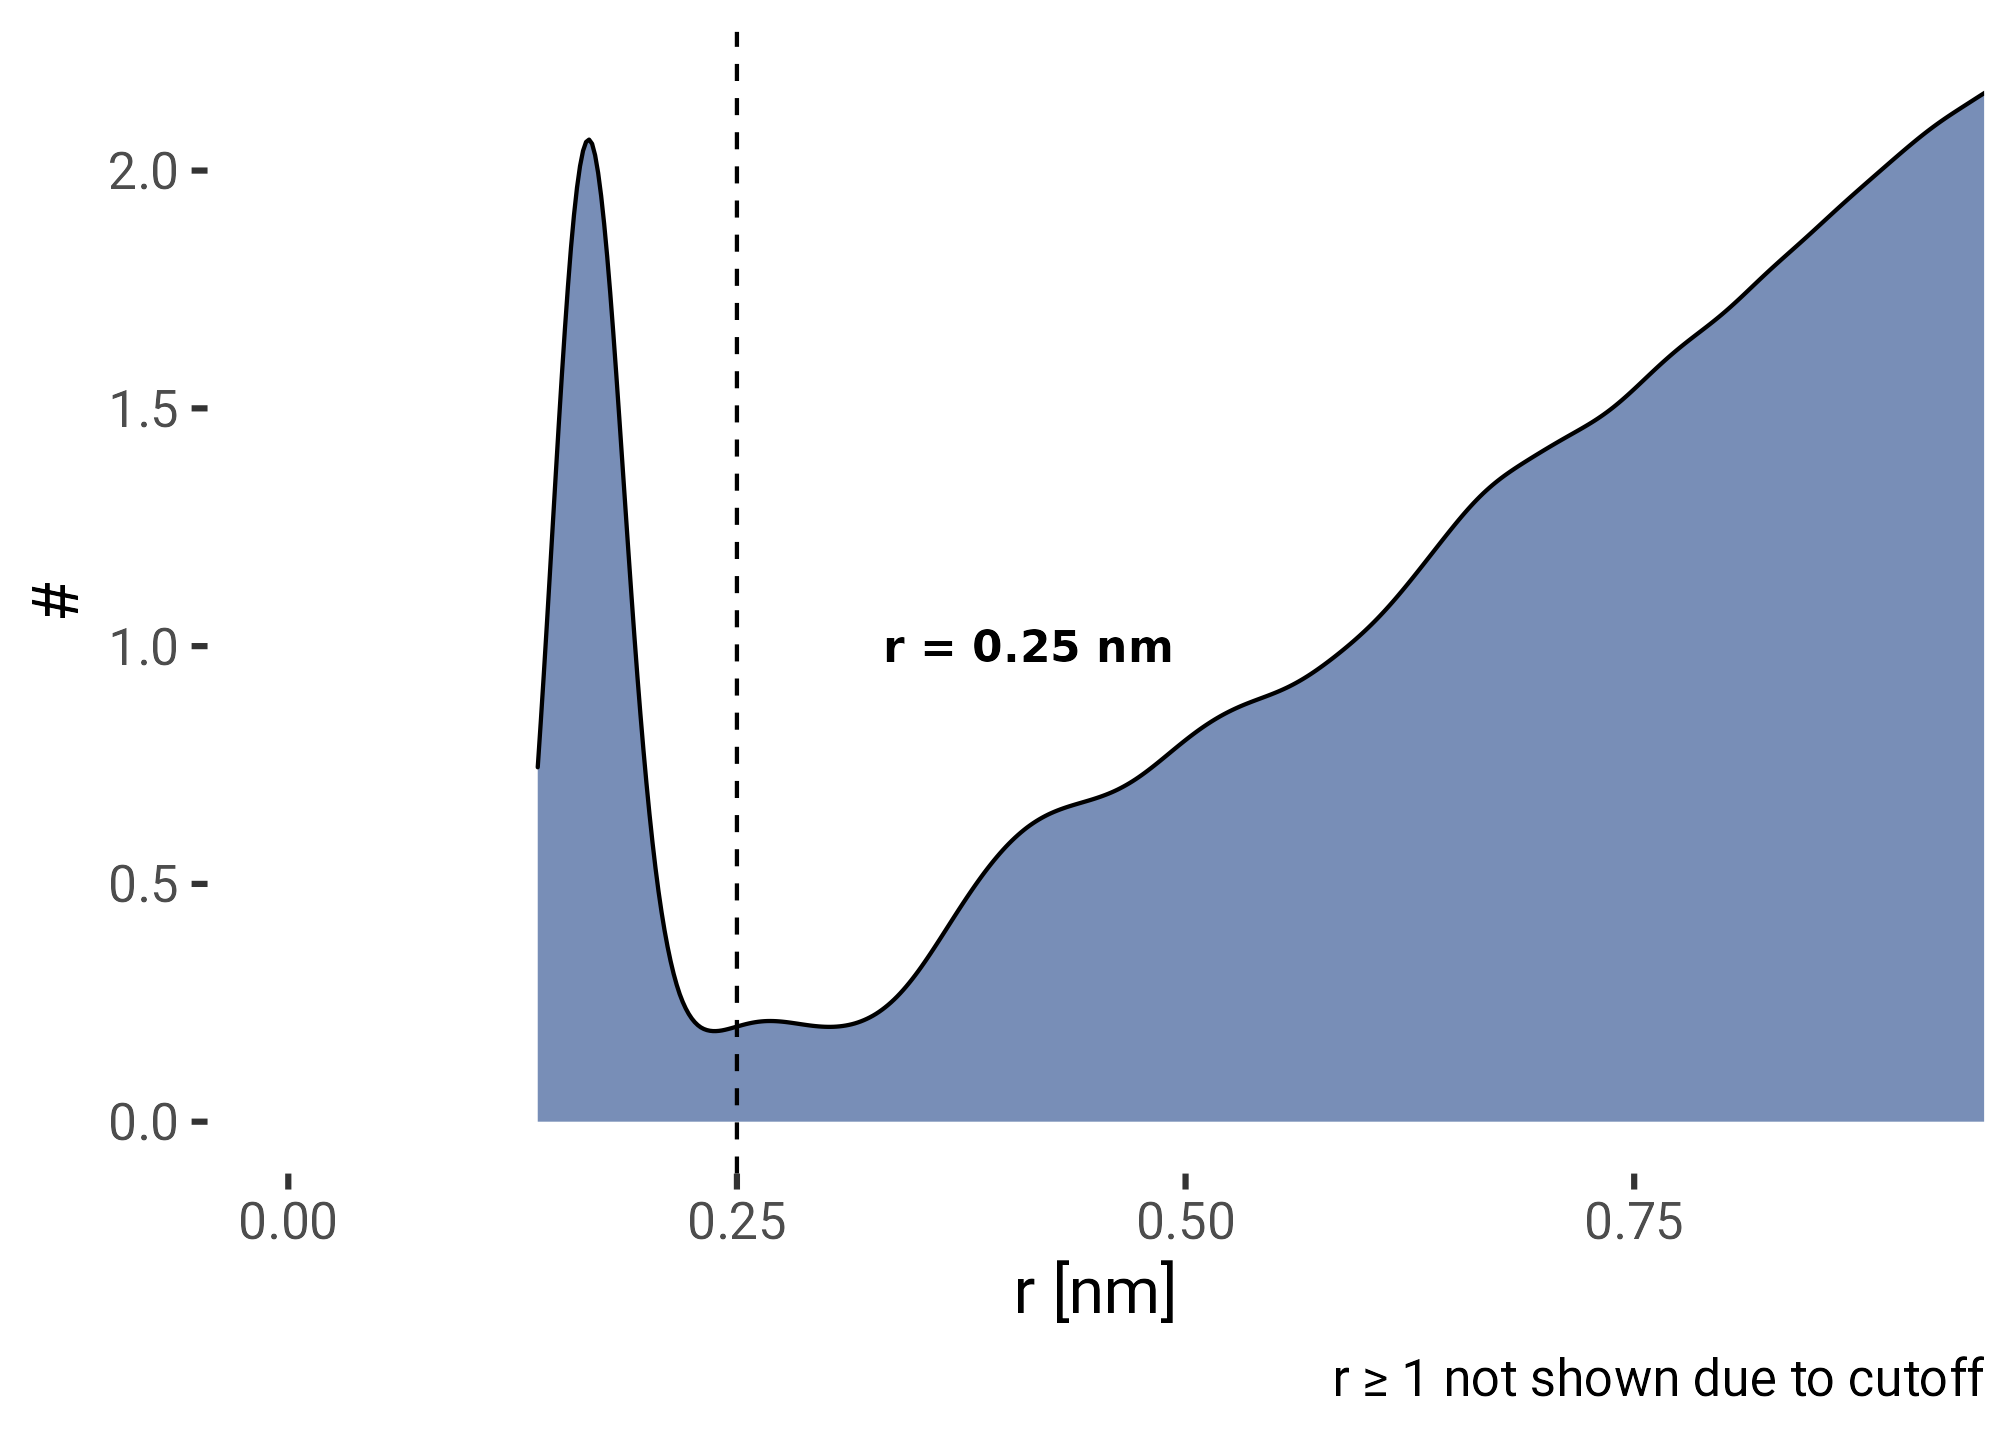
\includegraphics{./results/plots/f0f1-distance-cutoff-1.png}

}

}

\subcaption{\label{fig-r-hist}~}
\end{minipage}%
\newline
\begin{minipage}[t]{0.50\linewidth}

{\centering 

\raisebox{-\height}{

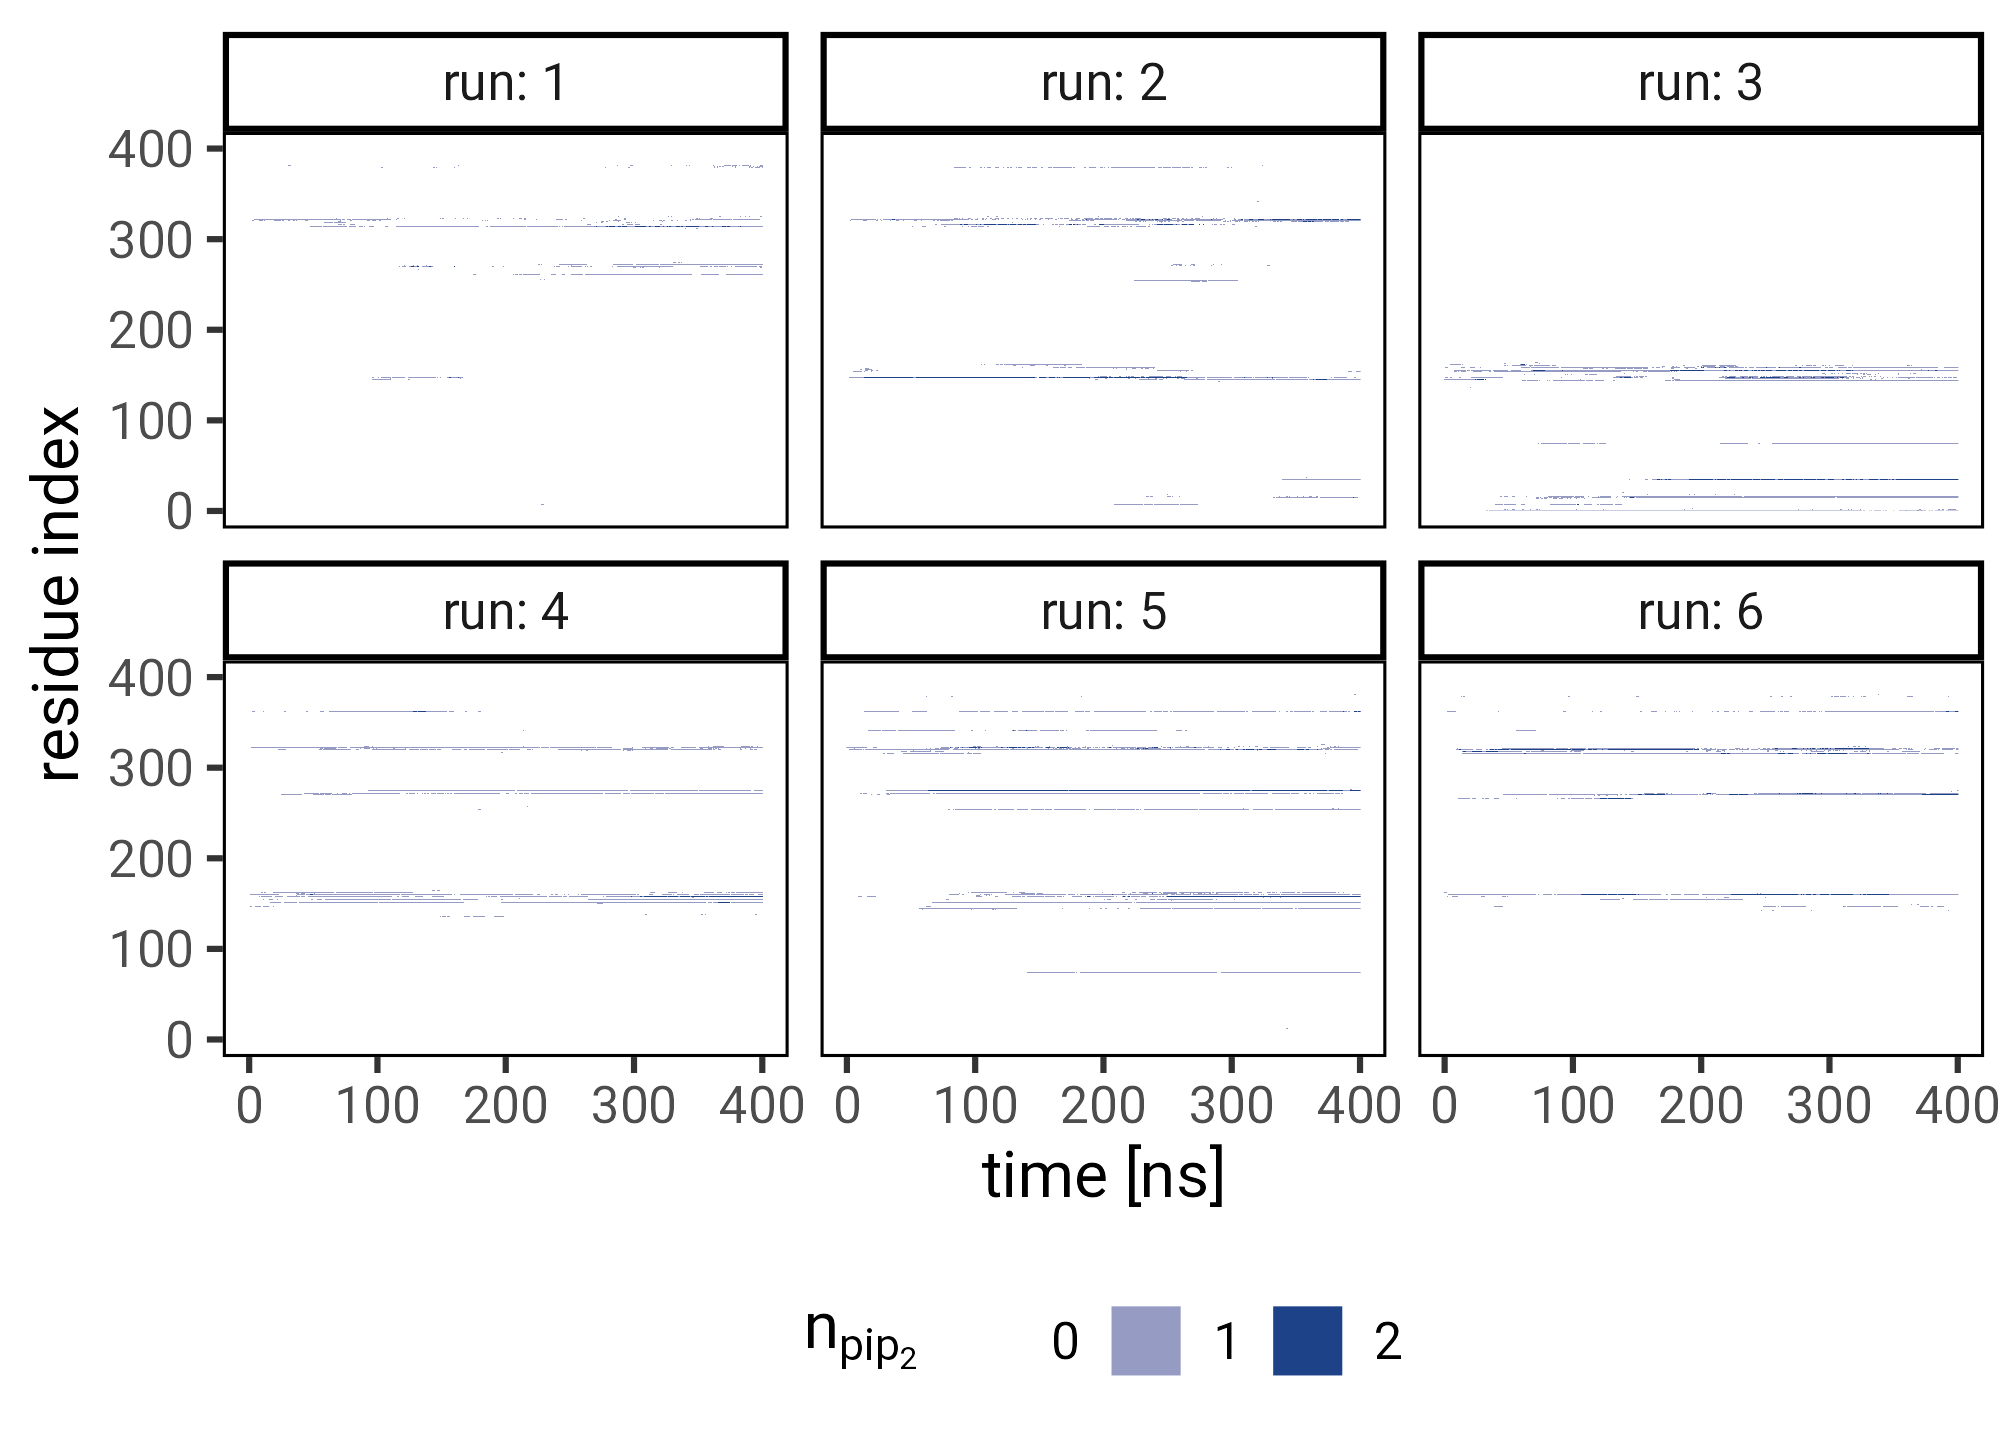
\includegraphics{./results/plots/ferm-time-ri-npip-all-1.png}

}

}

\subcaption{\label{fig-ferm-time-ri-npip-all}~}
\end{minipage}%
%
\begin{minipage}[t]{0.50\linewidth}

{\centering 

\raisebox{-\height}{

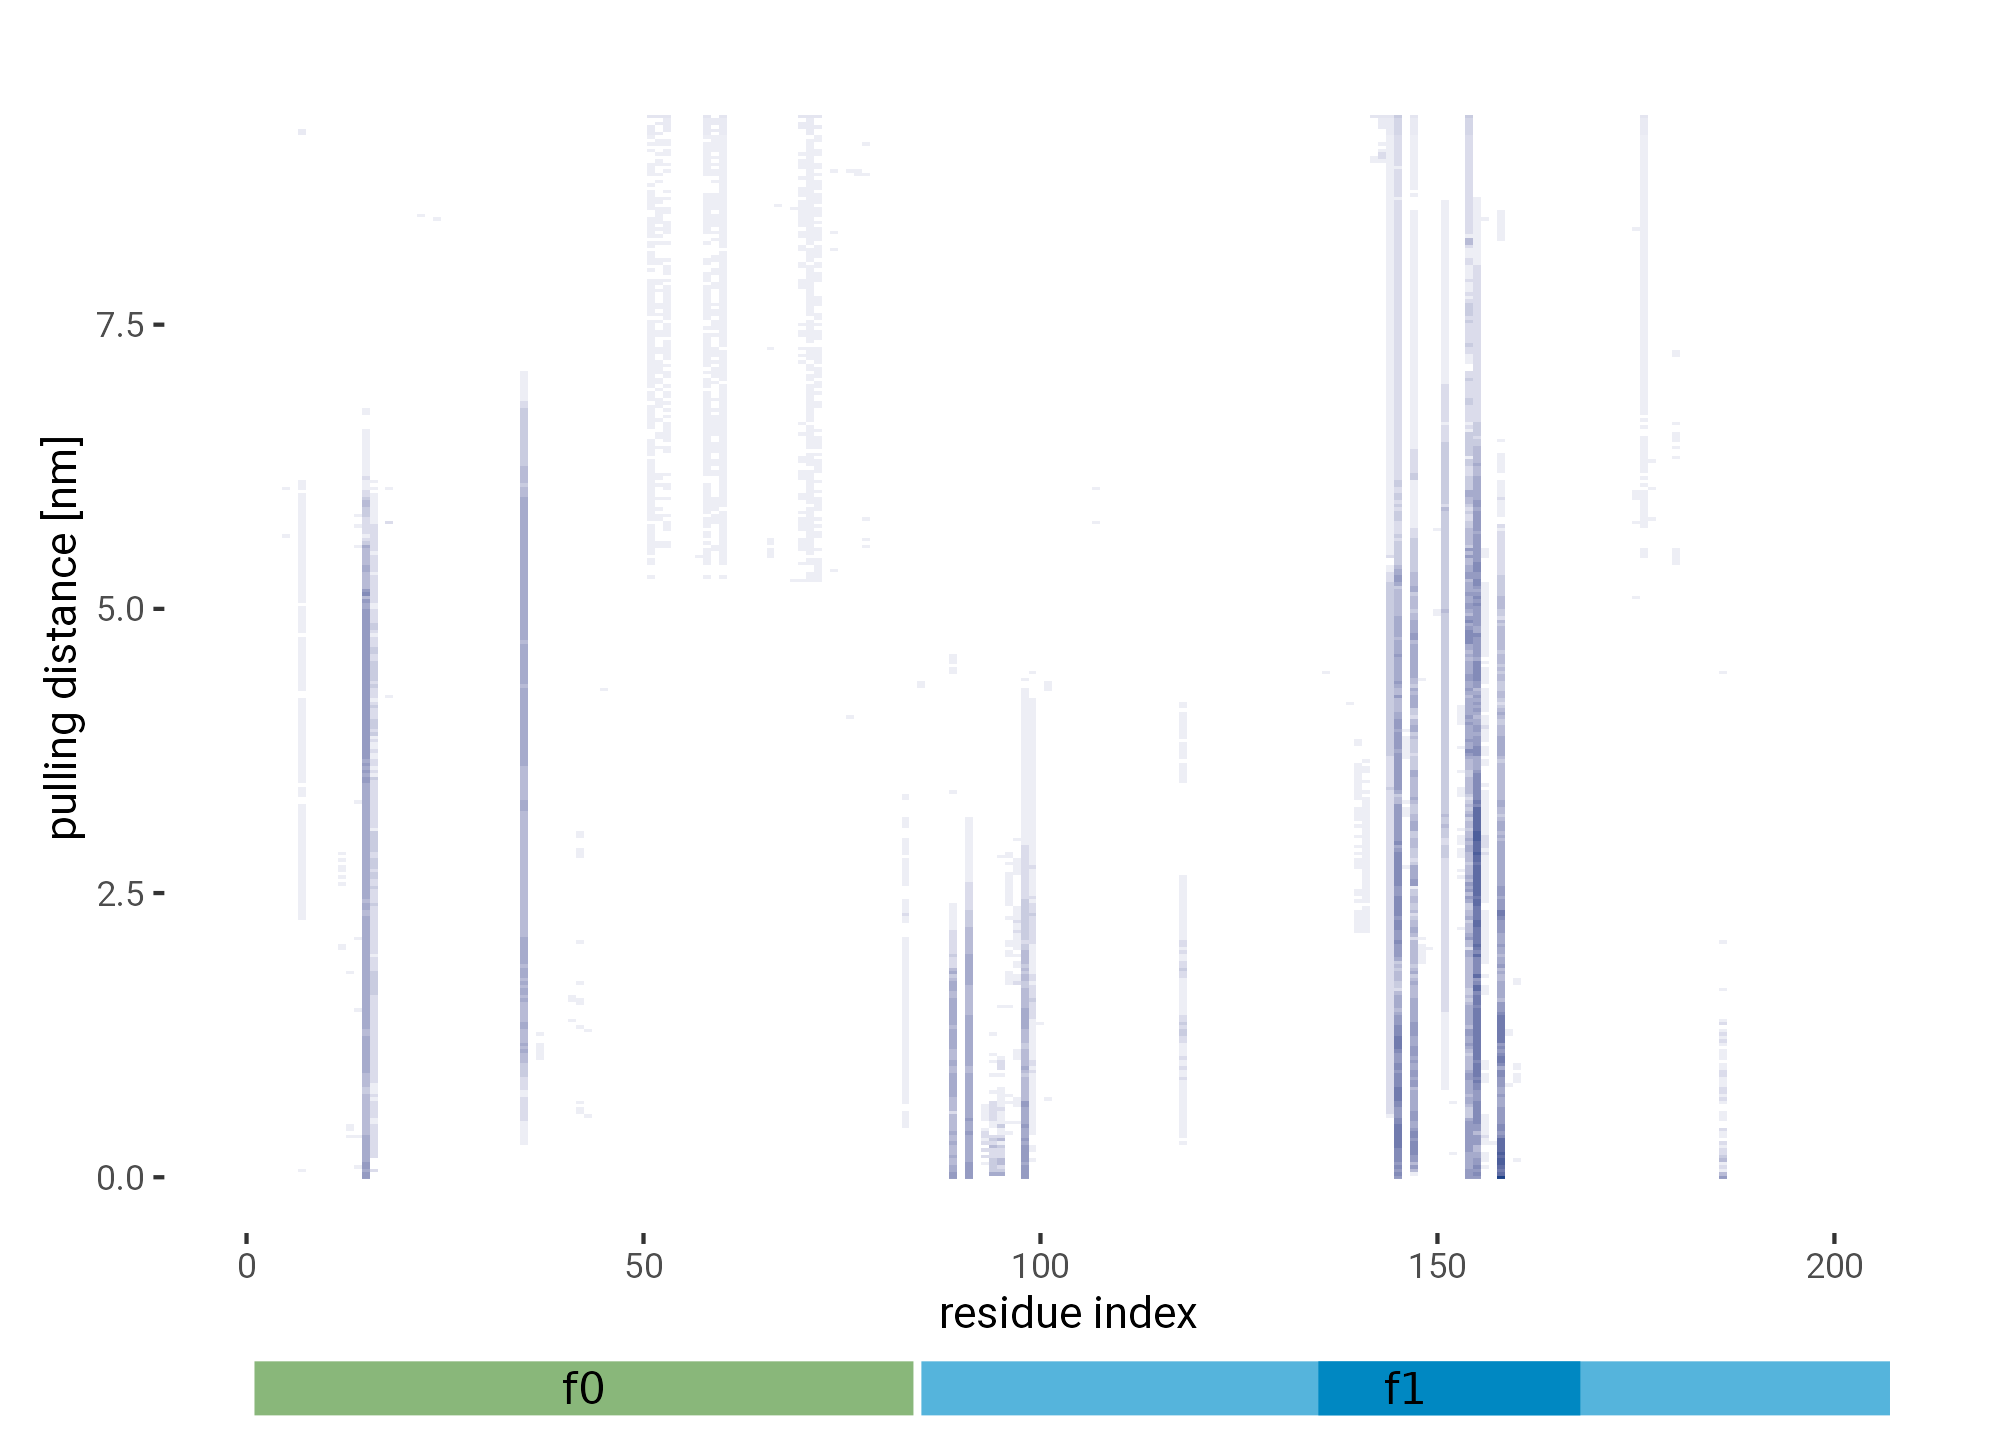
\includegraphics{./results/plots/f0f1-vert-pull-residues-1.png}

}

}

\subcaption{\label{fig-f0f1-vert-pull-residues}~}
\end{minipage}%
\newline
\begin{minipage}[t]{\linewidth}

{\centering 

\raisebox{-\height}{

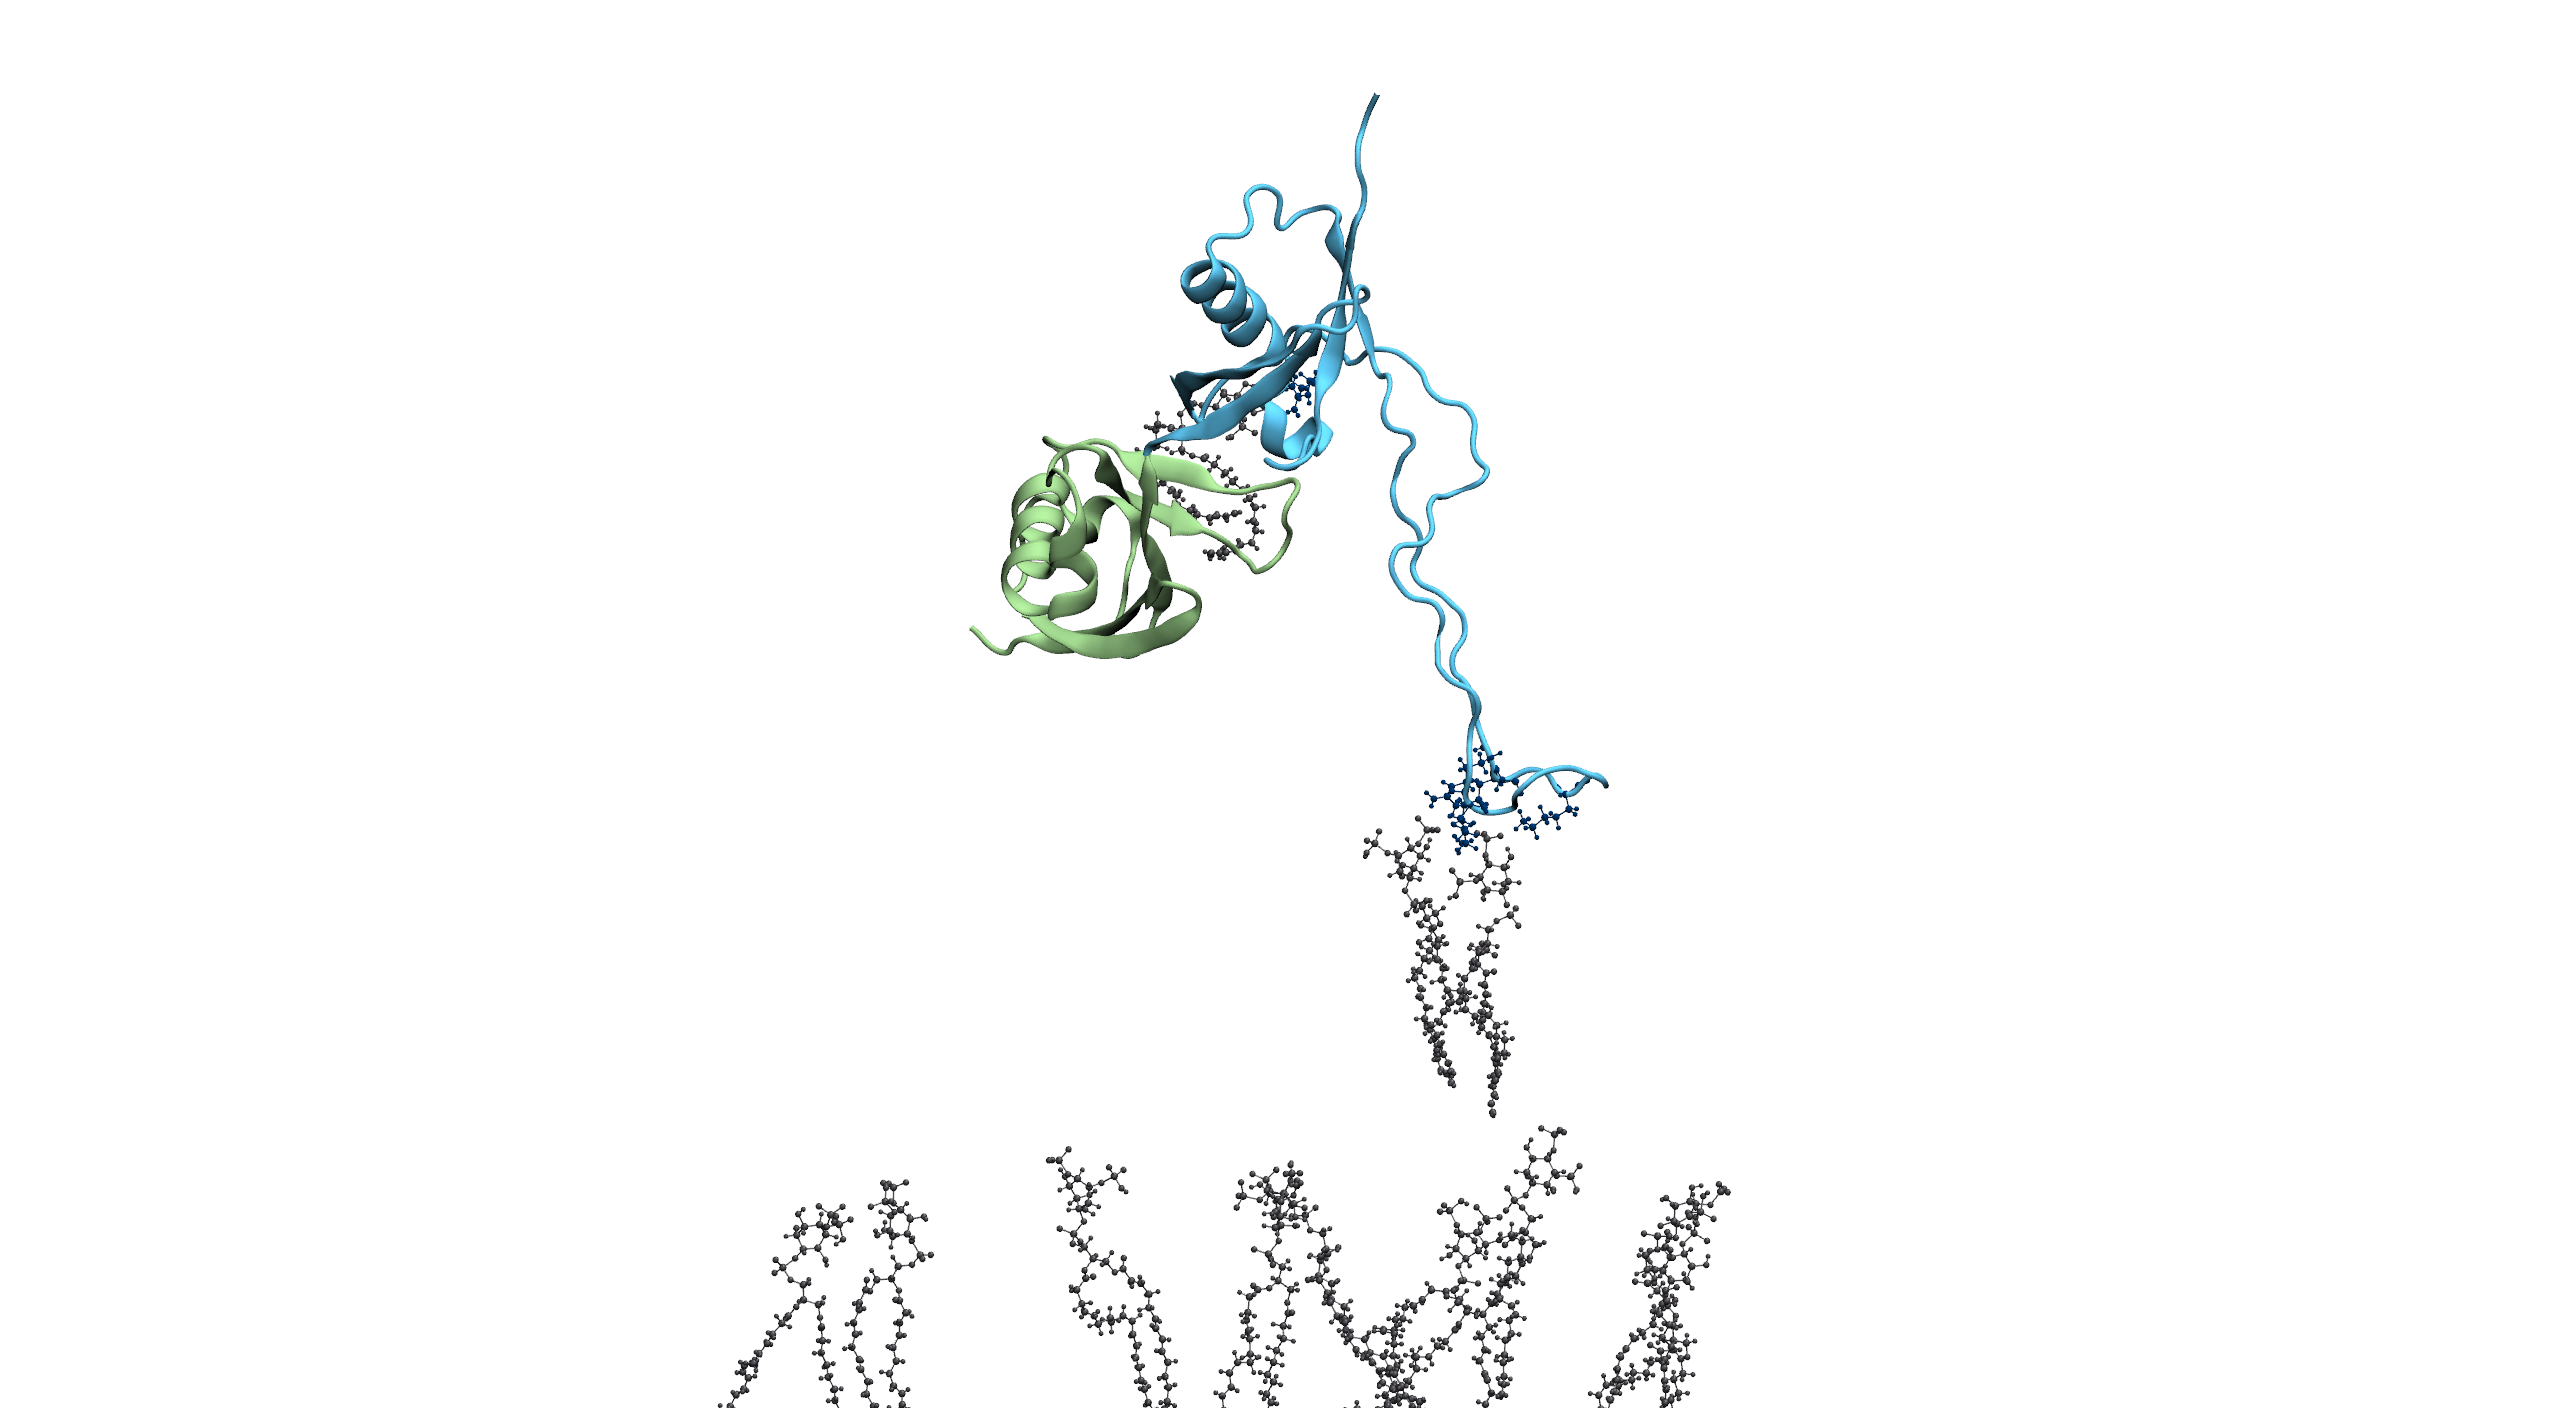
\includegraphics{./assets/vmd/f0f1-pulling/snapshot-run4.png}

}

}

\subcaption{\label{fig-f0f1-vert-pull-run4}~}
\end{minipage}%

\caption{\label{fig-suppl}\textbf{a)} RMSF {[}nm{]} of the c\(\alpha\)
of individual residues in an equilibrium simulation shown by coloring
the backbone The loop is highly flexible. \textbf{b)} A density plot of
distances between PIP\textsubscript{2} and the protein residues to
decide on a cutoff for defining interactions A distance of 0.25 nm was
chosen. \textbf{d)} A closer look at the residues involved in the
interaction during pulling reveals the instrumental role of both the F1
loop as well as the F0 subdomain in keeping the connection to the
membrane. \textbf{e)} Run 4 of the vertical pulling of F0F1.
Interactions between the protein and PIP\textsubscript{2} were so strong
that a total of 3 molecules of PIP\textsubscript{2} (gray) were pulled
out of the membrane (1 by F0 (green) and 2 by the F1 loop (blue)).}

\end{figure}

\hypertarget{tbl-f0f1-top-interacting}{}
\begin{longtable}[]{@{}lr@{}}
\caption{\label{tbl-f0f1-top-interacting}Top residues interacting with
F0F1}\tabularnewline
\toprule()
Residue & Mean \#PIP\textsubscript{2} \\
\midrule()
\endfirsthead
\toprule()
Residue & Mean \#PIP\textsubscript{2} \\
\midrule()
\endhead
M 1 & 0.188 \\
K 15 & 0.184 \\
R 30 & 0.173 \\
R 35 & 0.245 \\
R 74 & 0.124 \\
K 98 & 0.176 \\
R 118 & 0.209 \\
T 144 & 0.299 \\
L 145 & 0.168 \\
K 147 & 0.263 \\
L 151 & 0.325 \\
D 154 & 0.248 \\
E 155 & 0.261 \\
M 158 & 0.272 \\
K 160 & 0.254 \\
K 162 & 0.181 \\
L 193 & 0.200 \\
R 194 & 0.101 \\
\bottomrule()
\end{longtable}

\hypertarget{tbl-ferm-top-interacting}{}
\begin{longtable}[]{@{}lr@{}}
\caption{\label{tbl-ferm-top-interacting}Top residues interacting with
FERM}\tabularnewline
\toprule()
Residue & Mean \#PIP\textsubscript{2} \\
\midrule()
\endfirsthead
\toprule()
Residue & Mean \#PIP\textsubscript{2} \\
\midrule()
\endhead
M 1 & 0.118 \\
T 144 & 0.322 \\
L 145 & 0.129 \\
K 147 & 0.412 \\
L 151 & 0.204 \\
D 154 & 0.293 \\
E 155 & 0.257 \\
M 158 & 0.246 \\
K 160 & 0.459 \\
K 162 & 0.195 \\
Y 270 & 0.156 \\
K 272 & 0.180 \\
G 275 & 0.222 \\
L 314 & 0.141 \\
K 316 & 0.304 \\
K 318 & 0.148 \\
K 320 & 0.552 \\
G 321 & 0.174 \\
K 322 & 0.442 \\
D 341 & 0.142 \\
S 362 & 0.363 \\
\bottomrule()
\end{longtable}

\hypertarget{sec-prod-mdp}{%
\subsubsection{Molecular Dynamics Parameters}\label{sec-prod-mdp}}

\begin{Shaded}
\begin{Highlighting}[]
\ExtensionTok{integrator}\NormalTok{              = md}
\ExtensionTok{dt}\NormalTok{                      = 0.002}
\ExtensionTok{nsteps}\NormalTok{                  = 100000000}
\ExtensionTok{nstxout}\NormalTok{                 = 5000}
\ExtensionTok{nstvout}\NormalTok{                 = 5000}
\ExtensionTok{nstfout}\NormalTok{                 = 50000}
\ExtensionTok{nstcalcenergy}\NormalTok{           = 100}
\ExtensionTok{nstenergy}\NormalTok{               = 1000}
\ExtensionTok{nstlog}\NormalTok{                  = 1000}
\ExtensionTok{cutoff{-}scheme}\NormalTok{           = Verlet}
\ExtensionTok{nstlist}\NormalTok{                 = 20}
\ExtensionTok{rlist}\NormalTok{                   = 1.2}
\ExtensionTok{coulombtype}\NormalTok{             = pme}
\ExtensionTok{rcoulomb}\NormalTok{                = 1.2}
\ExtensionTok{vdwtype}\NormalTok{                 = Cut{-}off}
\ExtensionTok{vdw{-}modifier}\NormalTok{            = Force{-}switch}
\ExtensionTok{rvdw\_switch}\NormalTok{             = 1.0}
\ExtensionTok{rvdw}\NormalTok{                    = 1.2}
\ExtensionTok{tcoupl}\NormalTok{                  = Nose{-}Hoover}
\ExtensionTok{tc\_grps}\NormalTok{                 = SYSTEM}
\ExtensionTok{tau\_t}\NormalTok{                   = 1.0}
\ExtensionTok{ref\_t}\NormalTok{                   = 303.15}
\ExtensionTok{pcoupl}\NormalTok{                  = Parrinello{-}Rahman}
\ExtensionTok{pcoupltype}\NormalTok{              = semiisotropic}
\ExtensionTok{tau\_p}\NormalTok{                   = 5.0}
\ExtensionTok{compressibility}\NormalTok{         = 4.5e{-}5  4.5e{-}5}
\ExtensionTok{ref\_p}\NormalTok{                   = 1.0     1.0}
\ExtensionTok{constraints}\NormalTok{             = h{-}bonds}
\ExtensionTok{constraint\_algorithm}\NormalTok{    = LINCS}
\ExtensionTok{continuation}\NormalTok{            = yes}
\ExtensionTok{nstcomm}\NormalTok{                 = 100}
\ExtensionTok{comm\_mode}\NormalTok{               = linear}
\ExtensionTok{comm\_grps}\NormalTok{               = SYSTEM}
\ExtensionTok{refcoord\_scaling}\NormalTok{        = com}
\end{Highlighting}
\end{Shaded}




\end{document}
